%% 
%% Copyright 2007, 2008, 2009 Elsevier Ltd
%% 
%% This file is part of the 'Elsarticle Bundle'.
%% ---------------------------------------------
%% 
%% It may be distributed under the conditions of the LaTeX Project Public
%% License, either version 1.2 of this license or (at your option) any
%% later version.  The latest version of this license is in
%%    http://www.latex-project.org/lppl.txt
%% and version 1.2 or later is part of all distributions of LaTeX
%% version 1999/12/01 or later.
%% 
%% The list of all files belonging to the 'Elsarticle Bundle' is
%% given in the file `manifest.txt'.
%% 

%% Template article for Elsevier's document class `elsarticle'
%% with numbered style bibliographic references
%% SP 2008/03/01

%\documentclass[preprint,12pt]{elsarticle}

%% Use the option review to obtain double line spacing
%% \documentclass[authoryear,preprint,review,12pt]{elsarticle}
%%  \documentclass[2014,preprint,review,12pt]{elsarticle}

%% Use the options 1p,twocolumn; 3p; 3p,twocolumn; 5p; or 5p,twocolumn
%% for a journal layout:
% \documentclass[final,1p,times]{elsarticle}
%% \documentclass[final,1p,times,twocolumn]{elsarticle}
%% \documentclass[final,3p,times]{elsarticle}
%% \documentclass[final,3p,times,twocolumn]{elsarticle}

%% \documentclass[final,5p,times,twocolumn]{elsarticle}

%% For including figures, graphicx.sty has been loaded in
%% elsarticle.cls. If you prefer to use the old commands
%% please give \usepackage{epsfig}

%% The amssymb package provides various useful mathematical symbols

%% The amsthm package provides extended theorem environments
%% \usepackage{amsthm}

%% The lineno packages adds line numbers. Start line numbering with
%% \begin{linenumbers}, end it with \end{linenumbers}. Or switch it on
%% for the whole article with \linenumbers.
%% \usepackage{lineno}

%% Title, authors and addresses

%% use the tnoteref command within \title for footnotes;
%% use the tnotetext command for theassociated footnote;
%% use the fnref command within \author or \address for footnotes;
%% use the fntext command for theassociated footnote;
%% use the corref command within \author for corresponding author footnotes;
%% use the cortext command for theassociated footnote;
%% use the ead command for the email address,
%% and the form \ead[url] for the home page:
%% \title{Title\tnoteref{label1}}
%% \tnotetext[label1]{}
%% \author{Name\corref{cor1}\fnref{label2}}
%% \ead{email address}
%% \ead[url]{home page}
%% \fntext[label2]{}
%% \cortext[cor1]{}
%% \address{Address\fnref{label3}}
%% \fntext[label3]{}


%% use optional labels to link authors explicitly to addresses:
%% \author[label1,label2]{}
%% \address[label1]{}
%% \address[label2]{}

% % % % % % % % % % % % % % % % % % % % % % % % % % % % % % % % % % % % % % % % % % % % % % % % % %
% % % % Preamble
% % % % % % % % % % % % % % % % % % % % % % % % % % % % % % % % % % % % % % % % % % % % % % % % % %
\documentclass[preprint,5p,times]{elsarticle}
%\documentclass[2015,preprint,review,12pt]{elsarticle}
%%%%%%%\usepackage{amssymb}
%%%%%%%\usepackage{amsmath}
%%%%%%%\usepackage{epsfig}
%%%%%%%\usepackage{url}
%%%%%%%\usepackage{float}
\journal{International Journal of Impact Engineering}
\usepackage{graphicx}
\usepackage{mathptmx}
\usepackage[font=small,format=hang,labelfont=bf]{caption} 
\usepackage{gensymb}
\usepackage{enumerate}
\usepackage{epigraph}
\usepackage{titlesec}
\usepackage{cleveref}
\usepackage{scrextend}
\usepackage[english]{babel}
\usepackage[normalem]{ulem}
\usepackage{setspace}
\onehalfspacing
%\doublespacing
%From elsevier
\usepackage{amssymb}
\usepackage{amsmath}
\usepackage{epsfig}
\usepackage{url}
\usepackage{float}
\usepackage{tabularx}
\usepackage{cancel}
\usepackage{booktabs}
\usepackage{subfigure}
\usepackage{units}

%\hyphenation{*LOAD\_-BLAST\_-ENHANCED}
\begin{document}
% % % % % % % % % % % % % % % % % % % % % % % % % % % % % % % % % % % % % % % % % % % % % % % % % %
% % % % Frontmatter (Authors/Abstract/Keywords)
% % % % % % % % % % % % % % % % % % % % % % % % % % % % % % % % % % % % % % % % % % % % % % % % % %
\begin{frontmatter}
%\title{Numerical modelling of the structural response of welded materials under complex loading configurations. %panels subjected to air blast.
%Part I: Numerical modelling}
\title{Finite element based modelling of the structural response of welded materials in complex loading configurations. %panels subjected to air blast.
Part I: Structural modelling considerations}
\author[1]{A.J. Awang Draup \corref{cor1}}
\ead{jefri.draup@postgrad.manchester.ac.uk}
\author[1]{B. Rodgers}
\author[1]{J.D Robson}
\author[1]{P.B. Prangnell}
\author[1]{Q.M. Li}
\address[1]{The University of Manchester, Manchester, M13 9PL, UK}
\author[2]{M.J. Lunt}
\address[2]{DSTL, Porton, SP4 0JQ, UK}
\cortext[cor1]{Corresponding author. Tel: +44 (0)161 306 3578 Ext. 2261}

\begin{abstract}
This two-part article presents the results of numerical  prediction and experimental studies which aim to determine the structural response of friction stir welded aluminium 2139-T8 subjected to complex loading configurations, and in particular, air blast loading. The aim of this work is to develop a numerical modelling methodology to allow detailed prediction of the local strain evolution across the weld zone as this has significant influence in relation to structural response and failure. In particular, the method allows local material property gradients, which are due to variation in strengthening mechanism arising from microstructural damage caused by thermal loading during the welding process, to be incorporated into a macro scale structural model. Part I details the methodology used to implement local material property gradients together with experimental evidence to verify the predicted structural response in a range of loading configurations. Part II provides an insight into the assumptions made in Part I with respect to high strain rate materials modelling across the weld zone and the associated evidence for the variation in strengthening mechanisms in the alloy. The work presented highlights the importance of accurate description of the variation in local material properties, particularly the work hardening rate, in determining the response of structures under blast loading.
\end{abstract}

\begin{keyword}
%% keywords here, in the form: keyword \sep keyword
Blast loading\sep Digital image correlation \sep Materials modelling \sep Finite element simulation \sep Materials characterisation
%% PACS codes here, in the form: \PACS code \sep code
%% MSC codes here, in the form: \MSC code \sep code
%% or \MSC[2008] code \sep code (2000 is the default)
\end{keyword}

\end{frontmatter}

% % % % % % % % % % % % % % % % % % % % % % % % % % % % % % % % % % % % % % % % % % % % % % % % % %
% % % % Introduction
% % % % % % % % % % % % % % % % % % % % % % % % % % % % % % % % % % % % % % % % % % % % % % % % % %
\section{Introduction}
\label{Intro}
%
%Weld modelling of blast of interest.\\Particularly case of failure/performance. \\ Application is plastic collapse of buildings, failure in structures.\\Typical methods in litereature
%subject to assumptions which induce error, require careful calibration and interpretation.\\Particular important details are geometry, loading etc\\WRT mat props there is major simplification. typical approach\\implications in terms of range of model validity\\Propose a more detailed approach 
The structural performance of welded structures subjected to air blast loading is of key interest to engineers and scientists across a range of industries. For civilian applications, typically the risk of air blast is due to gas explosions and is an important design consideration in the construction of offshore oil platforms \cite{Langdon2005,Langdon2005a,Langdon2006}. %; 
%Other areas include the risk of gas ingress and explosion in domestic properties. 
%another consideration may be the risk of terrorist attack using explosives in public buildings. 
A key consideration here is not necessarily just the initial damage from the blast loading, but the risk of subsequent injury from collapse of the remaining structure. For steel framed buildings that are common in civil engineering, plastic deformation in the joints, which may be manufactured by welding, can be the limiting factor controlling structural integrity \cite{Ngo2007}. Detailed understanding of this localised damage is extremely important when considering the potential resistance of a building to blast and, therefore, any required mitigating engineering works to reinforce the structure; this may have an impact on the cost or design layout of a structure.

For military applications, the use of welded joints is common in personnel transport vehicles. With an increase in the threat from Improvised Explosive Devices (IEDs), the performance of welded structures has come under scrutiny \cite{Ramasamy2011}. There has been a global trend towards the use of vehicles, such as the Mastiff, which are designed to be mine resistant \cite{Morse2011}. In critical areas of a typical vehicle, such as the underbelly, the use of monolithic structures has become favourable as welds may lose integrity under blast loading. Local failure in the weld can lead to ingress of the explosive shock front into the vehicle, which can have catastrophic consequences on the occupants of the vehicle \cite{Ramasamy2011}. Indeed, it is unsurprising that one area of current research focus is on predictive techniques to aid the understanding of deformation and failure mechanisms in welded structures subjected to blast loading \cite{McWilliams2013,Grujicic2011a,Grujicic2012}.

Of course, in order to model the non-linear behaviour of a welded structure accurately, it is necessary to understand the interrelation between materials processing, material microstructure and the subsequent material and mechanical properties. Furthermore, the application of numerical modelling techniques, alongside the intrinsic errors arising due to the modelling assumptions made, need to be fully understood if a high fidelity model of weld behaviour is to be utilised and interpreted correctly.
%TODO Decide where this chunk of information should be put!
The scope of this paper limits discussion to structures manufactured via Friction Stir Welding (FSW), as described in \S\ref{IntroFSW}. Furthermore, discussion will be limited to heat treatable aluminium alloys, with particular reference to the alloy 2139-T8 as described in \S\ref{IntroAluminium2139t8}, though the general concepts are applicable across other alloys. Finally, consideration is only given to the Finite Element Method (FEM), as described in \S\ref{IntroWeldeModelling}, since it is widely used as a tool to study the response of structures under a wide range of loading conditions.
\subsection{Distribution of properties}
\label{LitRev:ModelStructuralQSMacroDistribution}

In addition to geometric variation in a welded structure (e.g. due to the formation of weld flash), and the formation of distinct geometric macro scale weld zones, both of which induce stress gradients, welding induces a meso-scale mechanical property variation across the weld zone. This is linked to the evolution of microstructure, and is extremely significant for age-hardenable aluminium alloys. Despite this known link, in all studies where the material property variation across the weld is modelled, all available evidence suggests that the local distribution is only resolved coarsely in each of the models \cite{McWilliams2013,Grujicic2011,Zhao2001,Zadpoor2009,Reis2004,Kim2010,Kim2010a}. Figure \ref{fig:FEMeshLumpedMass} shows a typical method for partitioning the weld zone into discrete regions, which simulate the HAZ, TMAZ, and nugget. Whilst the geometry of the weld zone is captured, all elements which are part of these individual are assigned one constitutive model that is assumed to be representative of the entire region. This means that the distribution of properties is homogeneous and isotropic within each region, and this shall be referred to as the ``lumped-mass" method. One feature of the the lumped-mass method, is that often the macro scale weld zones implemented into the mesh are calibrated to an experimental test \cite{Grujicic2011,McWilliams2013}, and some regions may be ignored altogether. The effect of using the lumped-mass method has not specifically been studied in the literature and shall be reviewed here.

\begin{figure}[h!]
	\centering
	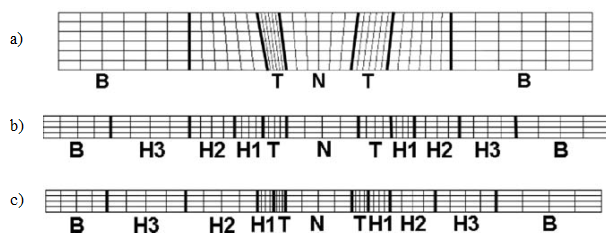
\includegraphics[width=0.75\linewidth]{Figures/LiteratureReview/FEMeshLumpedMass}
	\caption[Lumped mass method FE mesh]{Typical meshes generated using the lumped mass method for a) a 5251-O b) 2024-T351 c) 2024-T6. Figure adapted from Genevois et al. \cite{Genevois2006}}
	\label{fig:FEMeshLumpedMass}
\end{figure}
%
In some cases, this method is representative of the properties across the weld, such as non-age hardenable aluminium alloys subjected to FSW. As shown by Sato et al. \cite{Sato2001b}, for 1xxx and 5xxx alloys, the variation in both microstructure and mechanical properties is distinct across the weld. There is a distinct variation in the TMAZ and again in the nugget, which is related to the distinct variation in the contributions to hardening in those regions. Therefore, in this case, a discrete meso-scale distribution of mechanical properties in the elements, as illustrated in figure \ref{fig:FSWDistinctPropertyChange}, is a reasonably accurate description of physical reality. Moreover, this technique also requires a relatively small amount of computer memory as there are effectively only four material models to be referenced across the weld zone. However, as noted by McWilliams et al. \cite{McWilliams2013}, for age hardenable alloys, there are strong gradients in both yield stress and work hardening rates across the weld zone, which is linked to local microstructural variation \cite{Sato2001}. In their study conclusions, the authors mention that ideally, element-wise variation in yield stress would be a more appropriate way to specify material properties. 

This would enable accurate representation of the meso-scale yield stress variation across the weld. However, McWilliams et al. rightly point out that local work hardening response also demonstrates gradients across the weld, but that it does not scale simply with hardness. Therefore, in their study, the incorporation of a model which only accounts for yield stress variation is not justified because the additional accuracy in yield stress variation would be offset by an inaccuracy in work hardening variation, particularly in light of the fact their method utilises directly measured mechanical properties. Additionally, specifying an element wise distribution of properties is a non-trivial task as most software is designed to assign groups of elements distinct properties \cite{Hallquist2006}. Hence, specifying property distributions must be done either manually or via the use of a user defined sub-routine, which is a complex task, particularly when dealing with complex geometries. Furthermore, this method is likely to utilise a greater amount of computer memory because the number of constitutive models would relate to the element density, hence, the active variables stored in computer memory during each time step will be large. 

\begin{figure}[h!]
	\centering
	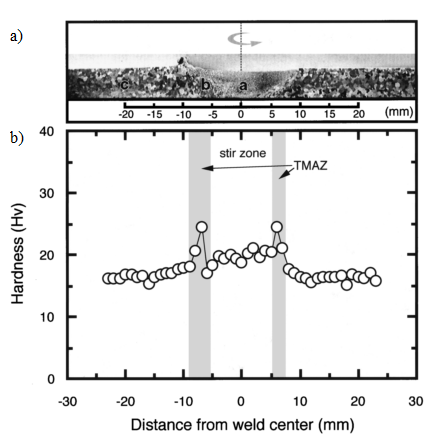
\includegraphics[width=0.6\linewidth]{Figures/LiteratureReview/FSWDistinctPropertyChange}
	\caption[Distinct property changes in FSW]{a) The cross section of 1080-O after FSW and b) the hardness variation across the weld. This shows that there is a distinct change in properties in the TMAZ and a distinct change in properties in the nugget. Figure adapted from Sato et al. \cite{Sato2001b}}
	\label{fig:FSWDistinctPropertyChange}
\end{figure}

In conjunction with a fundamental understanding of the FEM, two major observations of the effect of the lumped-mass method on numerical prediction of strain distribution for studies in the public domain can be made. Firstly, this method appears to lead to severe discontinuities in strain at the interfaces of the macro scale weld zones (i.e. HAZ, TMAZ, etc.). Secondly, an artificial double strain localisation is predicted to occur in the weld under uniaxial loading conditions. The occurrence of the severe strain discontinuities can be explained by considering the property change in the elements, as shown in figure \ref{fig:FEStepChange}. On the left hand side, the elements are assigned a relatively high yield stress, whereas the elements on the right are assigned a relatively low yield stress. Both sets of elements share a set of common nodes, which induces an artificial constraint on the elements with lower yield stress. Under loading, the elements with higher yield stress will deform slightly due to Poisson contraction under loading, whereas the elements with lower yield stress will deform more easily. However, at the interface the shared nodes are constrained to deform with the elements of higher yield stress. Effectively, the elements on the right hand side will demonstrate higher stiffness as they cannot deform as they would in reality, and is a problem similar to the use of fixed boundary conditions \cite{Hallquist2006,Systemes2010}. 

As mentioned in \S\ref{LitRev:ModelStructuralQSBC}, boundary conditions should be located as far as possible from the region of interest, but at the interface of the macro scale weld region this artificial constraint is located within the region of interest. Hence, it is possible that the solution in the region of interest is significantly affected by this constraint. Moreover, an increasingly fine mesh size is likely to exacerbate the effect because smaller elements are more sensitive to nodal displacement. This problem is intrinsic to the FEM and can be mitigated by minimising the mismatch in properties at the interface. This gives further support to the proposition to specify element wise yield stress variation by McWilliams et al. Figure \ref{fig:LumpedMassMcwilliams} shows the predicted strain distribution in a welded sample in comparison to the experimentally measured strain distribution by McWilliams et al. \cite{McWilliams2013} Quite clearly, at the boundary of the weld region interfaces, there is a significant discontinuity in strain. In this image, the exacerbation of strain discontinuity at the interface is not evident, which is likely due to the fact that strain contour plots generated by post-processing software are subject to a smoothing function. Figure \ref{fig:DoubleStrainLocalisation} shows the distribution of strain by Zadpoor et al. \cite{Zadpoor2009} and it is clear that, at the interface there is an increase in predicted strain, and an associated decrease towards the centre of the homogeneously modelled weld region. Genevois et al. \cite{Genevois2006} also utilise the method but appear to obtain close correlation between simulation and experimentation, as shown in figure \ref{fig:LumpedMassMatching}. However, the authors only present midpoint values for strain distribution predicted by FEM in comparison with their high resolution DIC measurements. In their study, the authors use a 1x1 mm resolution of elements to predict strain but a full set of elementwise predictions is not given. It is unclear whether or not the authors results would provide good matching, particularly at the weld interface. 

\begin{figure}[h!]
	\centering
	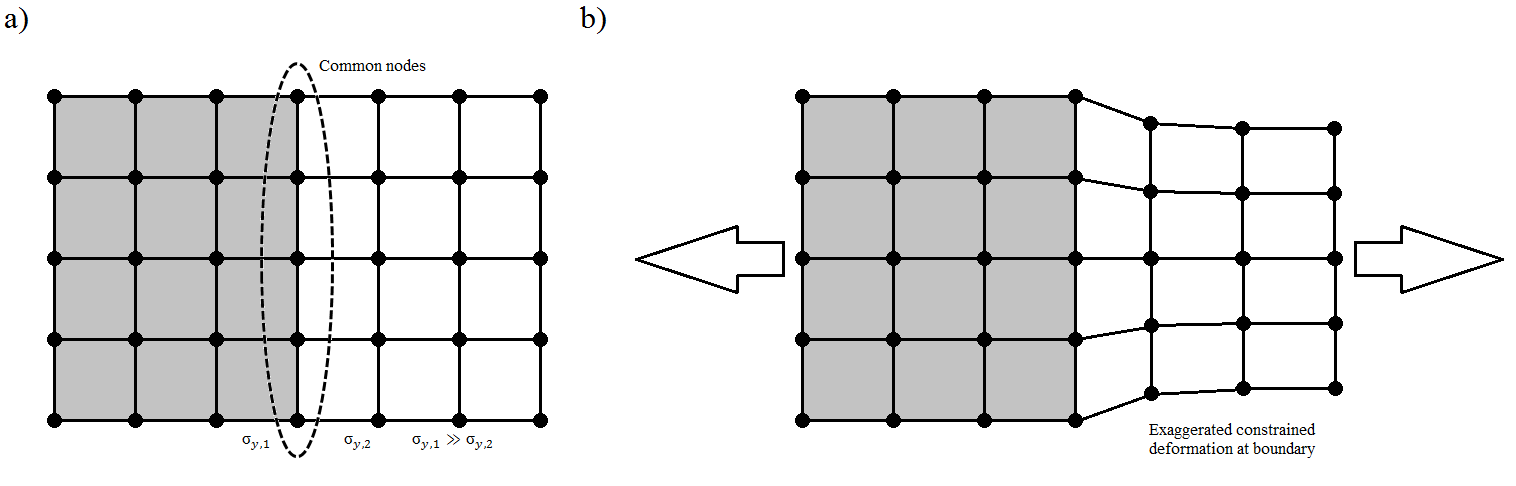
\includegraphics[width=1\linewidth]{Figures/LiteratureReview/FEStepChange}
	\caption[Constrained mesh deformation]{a) illustration of elements in a mesh with a distinct step change in properties. Elements share a set of common nodes at the boundary. b) The exaggerated effect of the step change in properties. The elements on the right are constrained by the elements on the left and effectively demonstrate an artificial increase in stiffness. This effect is exacerbated by increasing the step change in gradient.}
	\label{fig:FEStepChange}
\end{figure}

\begin{figure}[h!]
	\centering
	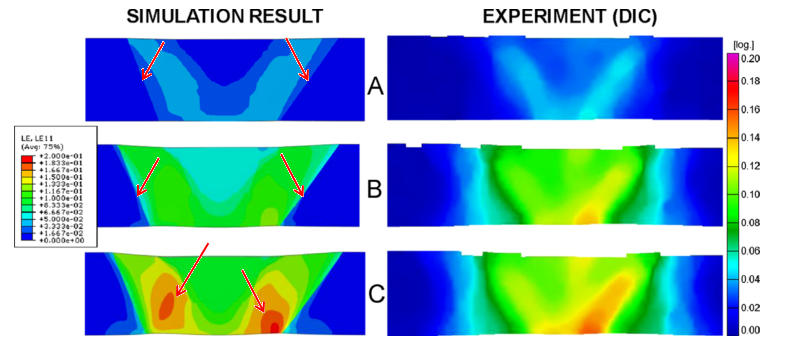
\includegraphics[width=1\linewidth]{Figures/LiteratureReview/LumpedMassMcwilliams}
	\caption[Lumped mass prediction]{The simulated strain prediction for FSW 2139-T8 loaded in uniaxial tension across the weld using the lumped mass method. Figure also shows the experimental measured strain measurements using DIC at the start, midpoint, and end of the test. There is a severe discontinuity in strain predicted at the boundaries of the weld zone and the simulation also predicts double strain localisation either side of the weld centreline, which does not occur in reality. Figure adapted from McWilliams et al. \cite{McWilliams2013}}
	\label{fig:LumpedMassMcwilliams}
\end{figure}

\begin{figure}[h!]
	\centering
	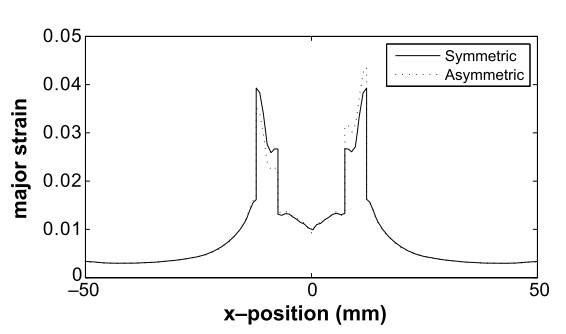
\includegraphics[width=0.75\linewidth]{Figures/LiteratureReview/DoubleStrainLocalisation}
	\caption[Strain prediction under biaxial loading]{The double strain localisation as predicted using the FEM for sheet forming operations. Figure adapted from Zadpoor et al. \cite{Zadpoor2009}}
	\label{fig:DoubleStrainLocalisation}
\end{figure}

\begin{figure}[h!]
	\centering
	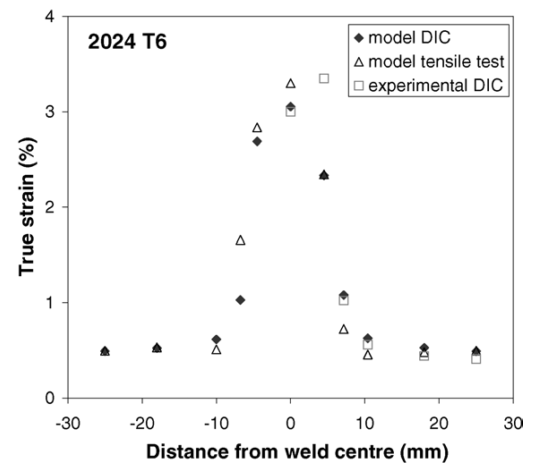
\includegraphics[width=0.75\linewidth]{Figures/LiteratureReview/LumpedMassMatching}
	\caption[Correlation using lumped mass method]{Predicted strain distribution using the lumped mass method and experimentally measured strain. It must be noted that in this case the simulations do not capture strain localisation which occurs in experiment. Figure adapted from Genevois et al. \cite{Genevois2006}}
	\label{fig:LumpedMassMatching}
\end{figure}

With respect to the double strain localisation effect, both figure \ref{fig:LumpedMassMcwilliams} and figure \ref{fig:DoubleStrainLocalisation} illustrate the development of strain either side of the weld centreline. It is unclear why this effect occurs, but it is possibly associated with the artificial constraints placed on the elements within narrow regions of the weld. By definition, any model which assumes weld symmetry or symmetric boundary conditions will generate double strain localisation either side of the weld. As shown in all experimental evidence reviewed in \S\ref{LitRev:FSWMPGlobalFracture}, under tensile loading, strain localisation and necking only occurs in one side of the weld \cite{Rhodes1997,Genevois2006}. In contrast, the double strain localisation effect can be seen in experimental evidence but only during the forming of Taylor welded blanks \cite{Zhao2001,Kim2010,Kim2010a}. It is possible that this phenomenon is linked to the stress conditions, which in the forming of sheets is approximately bi-axial in nature. Under compound loading, materials that demonstrate yielding according to the Von Mises criterion, which is an assumption usually implemented in commercial finite element software \cite{Hallquist2006,Systemes2010}, can support loads greater than the uniaxial yield stress, as shown by figure \ref{fig:VonMisesStrain}. Hence, it is possible that where material would normally yield on one side of the weld during uniaxial tension, due the constraints imposed under biaxial loading, greater stresses are supported throughout the weld, thus, large strains can localise either side of the weld centreline. %Grujicic et al. utilise the lumped-mass method to assess the performance of a welded structure under blast loading \cite{Grujicic2011} and simply extend a calibrated model of the weld in uniaxial tension to a more complex configuration. In this case, the authors achieved good qualitative correlation between a  predicted failure location and experimental measurement.

\begin{equation}
\label{eq:LR46}
\sigma_{VM} =\sqrt{\frac{1}{2}\bigg\{(\sigma_{1} - \sigma_2)^2 + (\sigma_2 - \sigma_3)^2 + (\sigma_3 - \sigma_1)^2\bigg\}}
\end{equation}

\begin{figure}[h!]
 	\centering
 	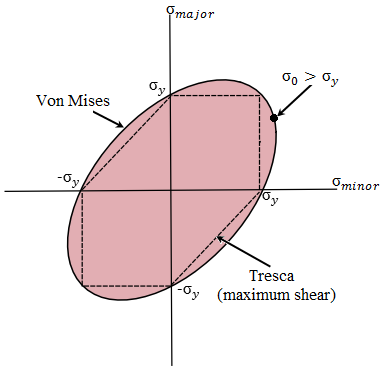
\includegraphics[width=0.5\linewidth]{Figures/LiteratureReview/VonMisesStrain}
 	\caption[Von Mises yield locus]{The theoretical yield locus, as described by equation \ref{eq:LR46}, under compound loading. The figure also illustrates the conservative yield estimate via the Tresca criterion, which is yielding under maximum shear.}
 	\label{fig:VonMisesStrain}
\end{figure}

In all studies reviewed here, highly detailed weld models were generated in order to assess structural failure or to implement mechanistic (micro-void growth and coalescence) models of failure into welds. However, the meso-scale mechanical property variation intrinsic to welds was only implemented at a much coarser resolution than other geometric details using the lumped-mass method. Given that the application of the lumped-mass method within the FEM is likely to induce erroneous local strain predictions, and only appears to provide correlation with experimentally measured strain distribution with the centre of the homogeneous weld regions, it is unclear whether or not the attempts by authors to incorporate complex anisotropic behaviour \cite{Kim2010,Kim2010a} or mechanistic failure models \cite{Chien2003a} will provide an objective understanding of the failure of welds under loading, as fracture is strongly linked to plastic strain history at any given point. 

\subsection{Weld Modelling}
\label{IntroWeldeModelling}
The typical method to study structural response to loading is to use the FEM and there are many instances of its use to study the response of welded structures \cite{Grujicic2011,McWilliams2013,Reis2004,Zhao2001}. However, successful macro scale modelling of weld behaviour under general loading conditions is extremely challenging as there are many factors which contribute to the overall structural behaviour. In addition to the variation in strengthening mechanisms across the weld zone (\S\ref{IntroFSW}), phenomena such as geometry misalignment from the welding process, the formation of weld defects, and residual stresses are all complexities which contribute to structural performance \cite{Kim2010,Grujicic2011a}. For example, residual stresses are known to adversely affect the fatigue life of welded structures. Moreover, correct application of modelling technique, such as definition of loading and boundary conditions is pertinent to model quality.  Whilst there has been a lot of work to improve FE based modelling methods with respect to some of the afore mentioned phenomena \cite{Zadpoor2009,McWilliams2013,Grujicic2011,Grujicic2010a}, a systematic approach to implementing local material property variation which arise due to welding process, which provides close quantitative correlation between prediction, has not emerged in the public domain. 
%there can be influence from local geometry variations due to misalignment of the welded plates or weld flash alongside complex residual stress fields induced by the welding process. Moreover, physical processes which occur on a micro scale significantly influence the material properties local to the weld zone, thereby generating structural variation and complexity on a meso-scale. 

In FEM based modelling, meso-scale complexity is typically dealt with by partitioning the mesh into distinct regions, which are representative of the weld regions (i.e. Nugget, TMAZ, HAZ and parent material) \cite{McWilliams2013,Grujicic2011}. Elements are assigned to these partitions and are collectively assigned homogeneous isotropic properties; these are usually defined by a Johnson-Cook material model:
\begin{equation}
\label{eq1}
\sigma = \bigg( A + B\epsilon^n_{p} \bigg)\; \bigg(1 +C\,\text{ln}\bigg(\frac{\dot{\epsilon}_{p}}{\dot{\epsilon}_{p0}}\bigg)\bigg)\; \bigg(1-\bigg(\frac{T-T_0}{T_m-T_0}\bigg)^m\bigg)
\end{equation}
It is common to assume that all parameters in equation \ref{eq1} are the same as the parent material except for the A parameter; this is assumed to scale linearly with hardness. The geometry of each region, such as the HAZ, may be defined by examination of the hardness distribution in the cross section of an actual weld or by visual inspection of metallographic specimens. However, it is common practice to calibrate the geometry of the model to experimental data from a real weld loaded in uniaxial tension. Usually, the calibrated model is extended to more complex structures and loading configurations without any further modifications \cite{McWilliams2013,Grujicic2011a}. This approach will hereby be referred to as the ``lumped-mass" method. 

It is widely known that in reality, there can be local variation to thermal and strain rate sensitivity or work hardening rate across the weld region \cite{Grujicic2011a,Genevois2006}. Since most weld models only account for yield stress variation across the weld important variation in material properties are neglected.
As a result, strong material property gradients, which can be diffuse in nature, are over simplified when implementing step functions through the use of the lumped-mass method \cite{McWilliams2013,Grujicic2011a}. Further, important material property gradients across the weld, in particular the work hardening rate are ignored. These simplifications make it difficult to obtain good matching between the predicted non-linear structural response and experimental data, local to the weld zone. Careful calibration of the partitioned zones is required in order to match the global non-linear response of the weld \cite{McWilliams2013,Grujicic2011a}. Moreover, it is unclear whether a model calibrated to a particular loading condition, specifically uniaxial tension, will accurately describe the structural behaviour under more complex loading conditions, such as blast loading of a plate. Data in the public domain reveal that structural models using the lumped-mass method only appear to show good qualitative correlation of structural behaviour of complex models calibrated to a more fundamental loading configuration; any supporting quantitative correlation is not reported \cite{McWilliams2013,Grujicic2011a}. 

\subsection{Summary}
\label{IntroSummary}
In this paper, an attempt to implement the strong material property gradients arising due to changes in strengthening mechanism, which is linked to variation in local material microstructure, is made. In Part I, focus is made on implementing local property gradients and the application of this technique to simulate the behaviour of FSW 2139-T8 under complex loading configurations including explosive air blast. Furthermore, experimental evidence that supports the predictions made is also presented here. With respect to developing the specific material models, namely the Johnson-Cook model, these are detailed specifically in Part II. 
%Variation in the local parameters defined is merely stated in Part I, with relevant microstructural evidence to justify the changes.

% % % % % % % % % % % % % % % % % % % % % % % % % % % % % % % % % % % % % % % % % % % % % % % % % %
% % % % Finite Element Modelling
% % % % % % % % % % % % % % % % % % % % % % % % % % % % % % % % % % % % % % % % % % % % % % % % % %
\section{Finite element modelling}
\label{FE}
Numerical modelling and simulation of welded panels was carried out using the commercial software package LS-DYNA version 971. In this study, the structural performance of welded material in loaded in uniaxial (cross weld) tension. The dynamic response of the structure was analysed using explicit time integration methodology. A displacement-based (Lagrangian) finite element analysis based on the virtual work principle was used to model the equations of motion. By integrating the equations of motion through time, the conditions within a discretised model of the system were determined. In particular, the non-linear evolution of plastic strain across the weld region was of interest as it is linked to failure \cite{Chien2003f}. 
%TODO P.S. Don't forget that you Need to mention hourglass control/control methodologies.
\subsection{Model Geometry}
\label{FEModelGeometry}
In this study, 1:1 scale models of the experimental apparatus were built manually using HyperMesh (Figure \ref{fig:UniaxialMesh}). For all simulations, the welded structures were assumed not to contain any weld defects, such as porosity, kissing bonds, or root defects. Furthermore, it was assumed that there was neither misalignment of geometry arising from the welding process, nor any local weld flash. These assumptions were appropriate as care was taken to ensure samples were properly aligned during the welding process and the samples were machined to final geometry before testing. In all cases, 8-node solid hexahedron elements were used. In the weld region, the element mesh had a resolution equivalent to 1x1x1 mm. 

\begin{figure}[h!]
	\centering
	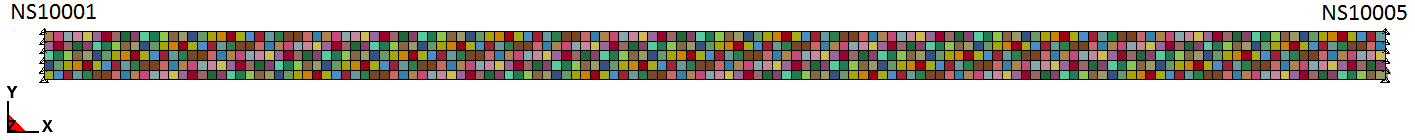
\includegraphics[width=1\linewidth]{uniaxial_load}
	\caption[Mesh]{Example finite element mesh that was generated using the method in \S \ref{FE}. Each colour code is indexed to a unique Johnson-Cook material modelled interpolated for the centroid of that element. The figure also highlights the node sets with boundary conditions specified in \S \ref{FEBoundaryConditions}}	
	\label{fig:UniaxialMesh}
\end{figure} 
\subsection{Material Properties}
\label{FEMaterialProperties}
%TODO change the description of this to equivalent of thesis
For all modelled parts, Johnson-Cook material models were used to define plastic behaviour accounting for strain rate and thermal sensitivity. In the region of the weld (where the local mesh resolution is 1x1x1mm) each element in the weld cross section is assigned a unique Johnson-Cook material model. This allows strong gradients of material properties to be defined across the weld. For each unique material model, the parameters for equation \ref{eq1} are defined based on the local thermal history, the post-weld hardness of the weld to be modelled, and mechanical property measurements obtained from ``simulated weld material", as indicated by equations \ref{eq2}-\ref{eq7}. By taking hardness measurements from three through thickness locations across the cross section of the weld in \S\ref{EMTensileTesting}, a map of hardness at the centroids of each element in the mesh can be interpolated from theses measurements, and used to define the meso-scale geometry of the weld since hardness is an indicator of $\textrm{f}_i(T,t,\vec{\textbf{x}})$ in the weld. Simulated weld material is generated by heat treating parent material using equivalent thermal cycles for positions locally across the weld using a methodology described by Shercliffe \cite{Shercliff1990,Shercliff1990a}; this method can also be used to predict the post-weld hardness of a weld \cite{Robson2006a,Sullivan2011}, which would allow prediction of weld structural response accounting for the welding parameters. Material property definition and, thus, meso-scale weld geometry is calibrated to a normalised weld condition rather than a particular loading configuration using this method, as is the case using the lumped-mass method. The Johnson-Cook parameters are shown to vary across the weld and are linked to changes in strengthening mechanism in response to the welding process. Further details of this method and experimental evidence for the link to strengthening mechanism variation are outlined in Part II the companion paper. An example of the parameters used to define material models for the elements across the weld cross section at the mid thickness of the plate are illustrated in figure \ref{fig:colormaps}.
\begin{equation}
\label{eq2}
%\begin{split}
%A&=k*Hv \textrm{\;Where\;} \\
%\label{eq2}
%k&=f(T,t)\\
%\label{eq3}
%B&=f(T,t)\\
%n&=f(T,t)\\
%C&=f(T,t)\\
%m&=f(T,t)
%\end{split}
A=k*Hv % \textrm{\;Where}
\end{equation}
\begin{equation}
\label{eq4}
B=\text{f}_1(T,t,\vec{\textbf{x}})
\end{equation}
\begin{equation}
\label{eq5}
n=\text{f}_2(T,t,\vec{\textbf{x}})
\end{equation}
\begin{equation}
\label{eq6}
C=\text{f}_3(T,t,\vec{\textbf{x}})
\end{equation}
\begin{equation}
\label{eq7}
m=\text{f}_4(T,t,\vec{\textbf{x}})
\end{equation}
Where
\begin{equation}
\label{eq3}
k=\text{f}_5(T,t,\vec{\textbf{x}})
\end{equation}
and $\vec{\textbf{x}}$ is the position of the element centroid within the welded sample; details are provided in Part II.

\begin{figure}
	\centering
	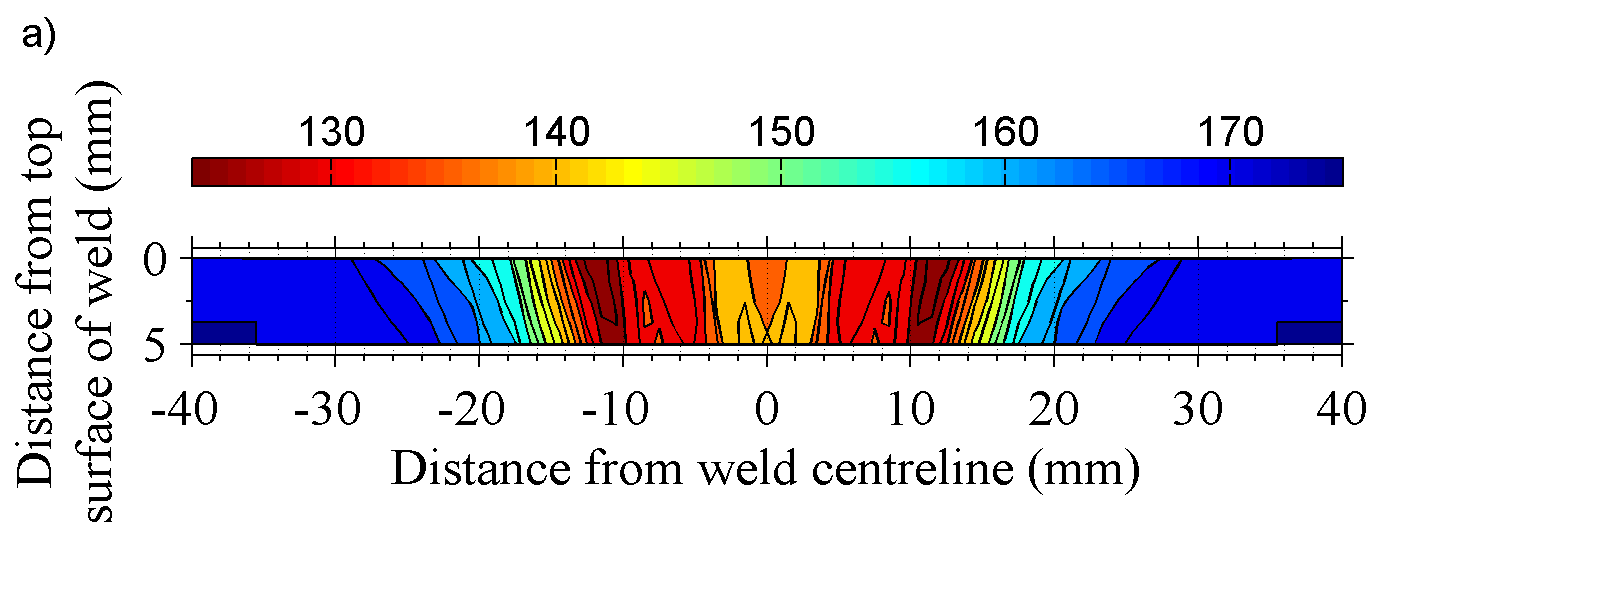
\includegraphics[width=1\linewidth]{JCHValtered}
	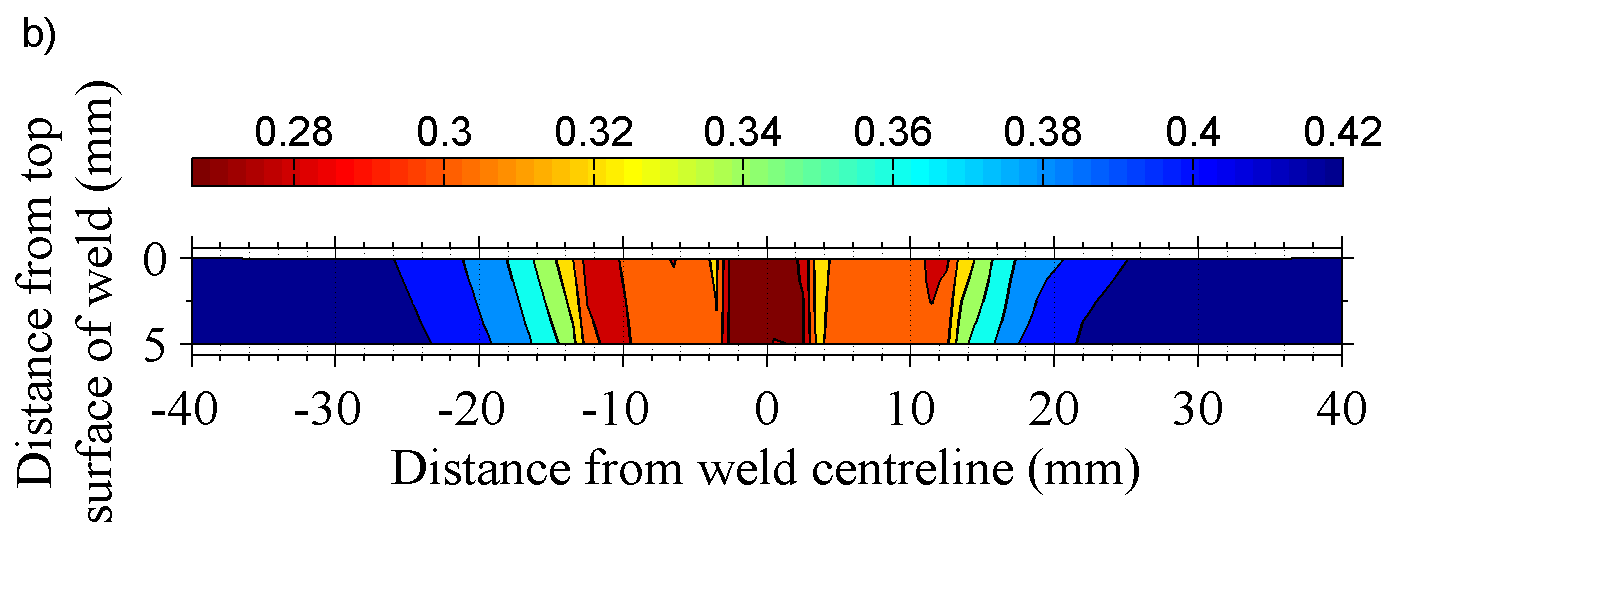
\includegraphics[width=1\linewidth]{JCAaltered}
	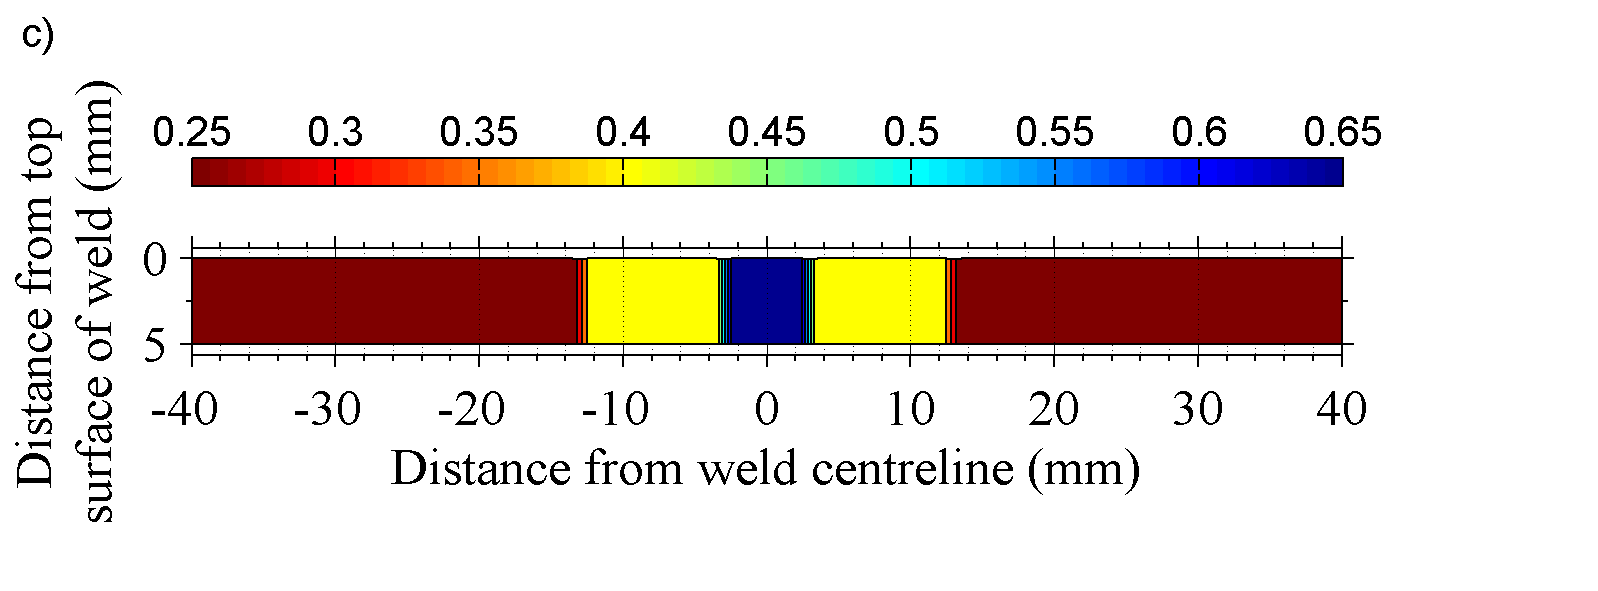
\includegraphics[width=1\linewidth]{JCBaltered}
	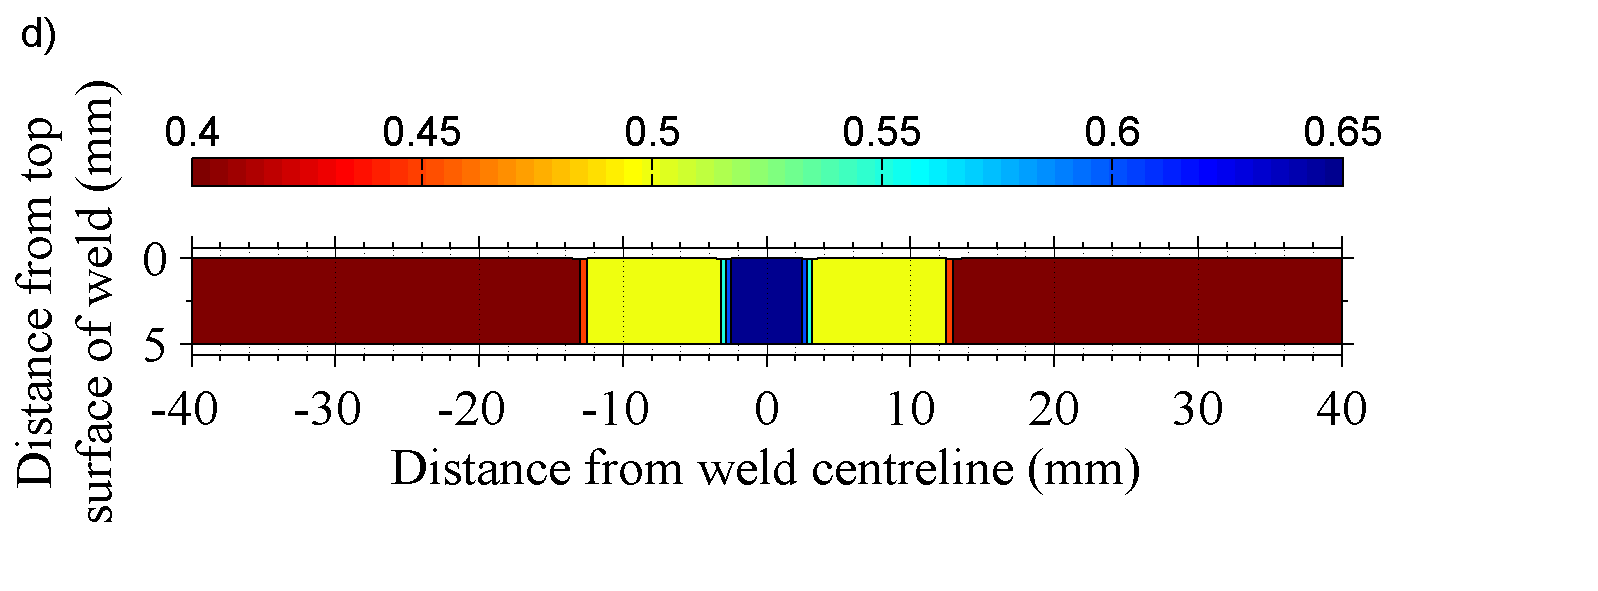
\includegraphics[width=1\linewidth]{JCnaltered}
	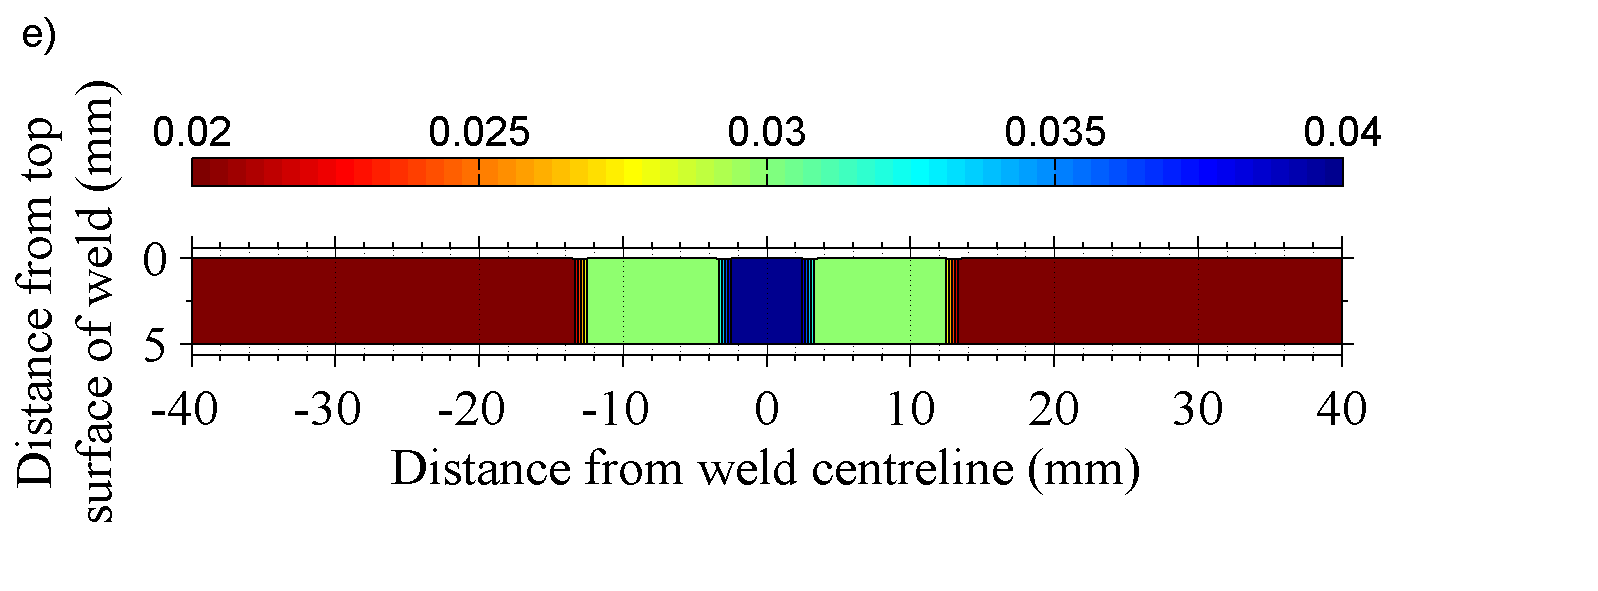
\includegraphics[width=1\linewidth]{JCCaltered}
	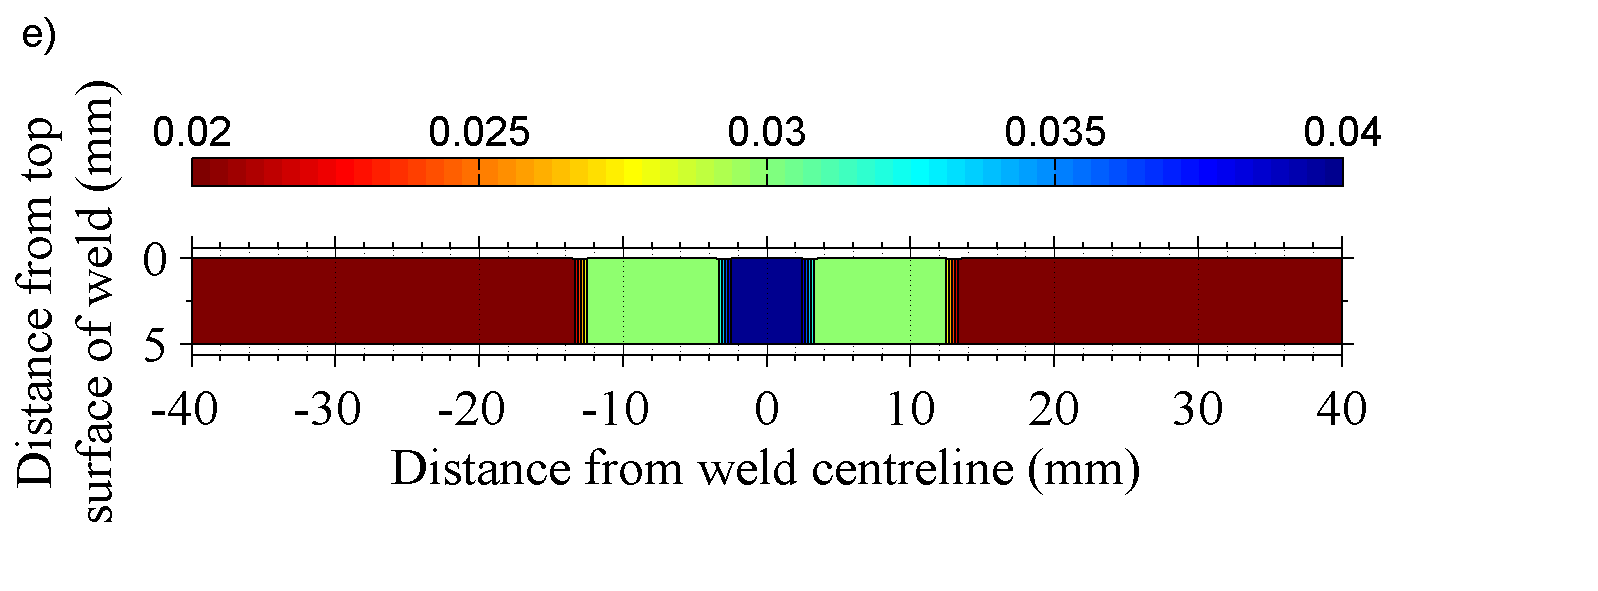
\includegraphics[width=1\linewidth]{JCCaltered}
	\caption[Mesh]{Element-wise distribution of properties interpolated across the weld cross section. a) Vickers Hardness b) Johnson-Cook A parameter (GPa). c) Johnson-Cook B parameter (GPa). d) Johnson-Cook n parameter. e) Johnson-Cook C parameter. f) Johnson-Cook m parameter.}
	\label{fig:colormaps}
\end{figure} 

\subsection{Loading Considerations}
\label{FELoadingConsiderations}
The presence of welding induced residual stresses has been neglected as it is assumed that they are relieved either during specimen preparation, when samples are sectioned from the welded plate, or during the initial stages of loading \cite{Peel2003}. Moreover, implementation of a representative residual stress profile in FSW 2139-T8 \cite{Grujicic2011a} in the modelled scenarios demonstrated negligible influence on the structural performance of the welds, though these have been omitted for brevity. Typically, residual stresses have influence over the propagation of cracks, and, hence, fatigue life of a structure rather than the deformation behaviour under loading \cite{Jata2000}. 

Loading due to gravity was ignored as these are small in comparison to the applied load and therefore unlikely to significantly affect the structural performance of the welds. Loading on the specimens was not explicitly defined using an applied external force, rather it was defined via the use of boundary conditions as detailed in \S\ref{FEBoundaryConditions}.

\subsection{Boundary Conditions}
\label{FEBoundaryConditions}
In the models of welds loaded in uniaxial tension, the nodes at the ends of the specimen were assigned a prescribed motion boundary condition (\url{*BOUNDARY_PRESCRIBED_MOTION} input card). The boundary conditions are illustrated in figure \ref{fig:UniaxialMesh}, and for the node set %at the left hand side of the image,
NS10001, the velocity is set to \textit{$u=0$} mm min\textsuperscript{-1}, whilst for the node set
% on the right hand side of the image
NS10005, the velocity is set to \textit{$u=1$} mm min\textsuperscript{-1}. This is equal to the velocity of the moving cross head on the tensile rig.

% % % % % % % % % % % % % % % % % % % % % % % % % % % % % % % % % % % % % % % % % % % % % % % % % %
% % % % Experimental MEthods
% % % % % % % % % % % % % % % % % % % % % % % % % % % % % % % % % % % % % % % % % % % % % % % % % %
\section{Experimental Methods}
\label{EM}
In order to test the validity of the modelling methods described in %TODO add section ref
the structural performance of welds under uniaxial loading was measured experimentally. The details of all the experimental methods used are presented below.
%TODO go through and check all cross referencing
\subsection{Welding parameters}
\label{EMTensileWeldParameters}
2139-T8 plates were supplied from Constellium and all welding was carried out with the plates in the as-received condition. Samples were rigidly clamped and were positioned in direct contact with a steel backing plate.

Plates were machined into a work-piece with dimensions 150 mm x 300 mm x 6.38 mm (RD x TD x ND). The work-piece was machined with pilot holes to allow thermocouples to be embedded within; this enabled the thermal history within the work-piece to be recorded during the welding process. The thermal data was utilised to validate the post-weld hardness model (\S\ref{RADMicrostructureCharModelHV} chapter \ref{ResultsMicrostructure}). 
Thermocouples were positioned at the centre of the plate (150 mm in RD) at a fixed depth, in the \textit{z}-direction (3 mm in ND), from the top surface of the plate and at increasing distance from the weld centreline (0 mm, 3 mm, 5 mm, 8 mm, and 12 mm in TD) \textit{x}-direction, as shown in figure \ref{fig:Thermocouples}. 

\begin{figure}
	\centering
	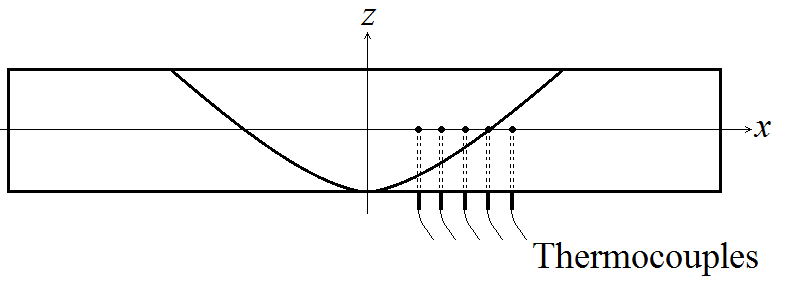
\includegraphics[width=0.65\linewidth]{Figures/ExperimentalMethods/Thermocouples}
	\caption[Thermocouple positions]{Schematic illustrating the position of thermocouples within the weld cross section.}	
	\label{fig:Thermocouples}
\end{figure} 

Welding was carried out with a conventional tool featuring a tri-flat tapered pin. The tool dimensions were: 18 mm shoulder diameter with a 2 \degree concave angle, 5.8 mm pin length featuring a pin root diameter of 6.2 mm and a pin tip diameter of 4.5 mm. Welding was carried out with a rake angle of 10 \degree, tool rotation speed of 1000 RPM and a tool advance speed of 100 $\text{mm}\!\cdot\!\text{min}^{-1}$. The initial plunge speed was set to 10 $\text{mm}\!\cdot\!\text{min}^{-1}$ and a dwell time of 10 s, whilst the tool extraction speed was set to 10 $\text{mm}\!\cdot\!\text{min}^{-1}$. In total, a weld of 200 mm length was carried out parallel to RD. The measured average tool downforce was approximately 20 kN. Welding was carried out by the University of Manchester with a Crawford-Swift FSW machine with the tool in position control mode.

%Bead on plate FSW was carried out on 2139-T8 alloy where the work-piece dimensions are 150x300x6.35 mm. Welding was carried out with a conventional tool with triflat pin set at a 2$^\circ$ rake angle. The tool dimensions were: 18 mm shoulder diameter; 2$^\circ$ shoulder concave angle; 6.2 mm pin root diameter; 5.85 mm pin height; 4 mm pin tip diameter. The weld settings were: 100 $\text{mm}\!\cdot\!\text{min}^{-1}$ traverse speed; 1000 RPM rotation speed; 16 kN downforce. The welds were carried out with the tool in force control mode. 
\subsection{Tensile Tesing of FSW 2139-T8}
\label{EMTensileTesting}
Square cross section bars with dimensions 5x5x150 mm were machined from the welded plates. By preparing samples in this way, geometry induced stress concentrations arising due to weld flash are eliminated as they are milled away. Further, residual stresses are relieved as the specimen is no longer constrained by the bulk material. This also simplifies the modelling process and allows the effects of material property gradients to be isolated during tests. Samples were tested using an Instron 5569 machine where the cross-head displacement rate was set to 2 $\text{mm}\!\cdot\!\text{min}^{-1}$. Testing was carried out according to BS6892-1:2009.
\subsection{Digital Image Correlation}
\label{EMDIC}
2D Digital Image Correlation (DIC)  \cite{DaFonseca2005} was performed on square bar tensile specimens which captured the full weld region in order to measure the strain response of the weld. A LaVision Imager Pro Plus 4M greyscale camera, fitted with a Nikon AF-D Micro-Nikkor 105 mm f/2.8 macro lens and a Nikon 2x teleconverter, was used to acquire images with a 2096x2096 pixel resolution at a frequency of 1 Hz. The test setup was illuminated using a 150 W halogen lamp positioned at a low angle to the sample to avoid direct reflection into the camera. 

The specimens were prepared for DIC by first systematically grinding the face of the sample to be imaged down to P180-P1200 grit. This ensures that the sample is flat, as required for 2D DIC, and has enough surface roughness to allow good adhesion between the paint and the sample surface. The surface was then thinly coated with a matte white surface primer; this prevents direct reflection of light into the camera. The sample was allowed to cure for 24 hours and was subsequently partially coated with a matt black spray paint. By partially coating the specimen, a unique speckle pattern forms naturally on the surface which can be analysed by the DIC software. The typical speckle feature size of the samples was approximately 3x3 pixels. DIC analysis was carried out using the commercial software package LaVision DaVis 8.1.5. A 2D time series cross correlation was carried out in integral mode using the sum of differential vector fields. Displacement calculation was performed with multi-pass iterations where the window sizes decrease from 128x128 pixels to 32x32 pixels. The final window had a circular Gaussian probability function fitted to the sub-regions to account for large strains and rotations; all subregions were located with 25\% overlap.

% % % % % % % % % % % % % % % % % % % % % % % % % % % % % % % % % % % % % % % % % % % % % % % % % %
% % % % Results and Discussions
% % % % % % % % % % % % % % % % % % % % % % % % % % % % % % % % % % % % % % % % % % % % % % % % % %
\section{Results}
\label{Results}
The relevant results and supporting discussion are split with reference to the particular loading condition studied. In particular, the focus of prediction and validation techniques pertains to the spatial and time evolution of plastic strain distribution across the weld. It is widely known that failure in ductile materials is often linked to the local plastic strain. In ductile materials, failure mechanisms such as formation of micro-voids, void coalescence and crack formation are heavily linked to plastic strain. Whilst there are many modelling methods which aim to predict these particular phenomena, they are not the focus of this study. The primary aim of the uniaxial tension study is to verify the prediction of strain distribution made using the modelling method in \S\ref{FEUniaxialTension}; the precise determination of failure is not considered. The primary aim of the blast loading study in \S\ref{EMBlastTesting} is to verify that the modelling method in \S\ref{FEBlastLoading} accurately captures the strain evolution when extended to complex loading configurations. Again the precise determination of failure is not considered.
%
%\subsection{Uniaxial Loading}
%\label{RADUniaxialLoading}
%The presented results can be understood upon examination of the material properties, which are linked to the strengthening mechanisms detailed in Part II. In this discussion, any variation in strengthening mechanisms shall be stated as all materials characterisation is discussed and justified in Part II. For the purposes of this discussion, the HAZ is split into the outer HAZ\footnote{approximately the region of the weld cross section defined by $40\geq|x|\geq12$ mm} and the inner HAZ\footnote{approximately the region of the weld cross section defined by $12\geq|x|\geq3$ mm}. The outer HAZ is the region between the hardness minima in the weld (see figure \ref{fig:colormaps}) and the parent material where the hardness value returns to that of the parent plate. The inner HAZ is the region bounded by the hardness minima in the weld and the dimensions of the tool pin. In this discussion the TMAZ is not treated as a distinct region in its own right, rather it is part of the inner HAZ. The nugget region is the region bounded by the dimensions of the tool pin\footnote{approximately the region of the weld cross section defined by $|x|\leq3$ mm}.
%
%On a macro scale, the evolution of strain is demonstrated in figure \ref{fig:UniaxialStrainMacro}, which shows the distribution of the strain component in the cross weld direction; this is hereby referred to as axial strain. Most prominently, the features of interest which correlate closely between prediction and experimental evidence are the  smooth gradients in strain in the outer regions of the weld; the correlation in strain throughout global deformation steps; and the single point of strain localisation in the weld. 
%\begin{figure}[h!]
%	\centering
%	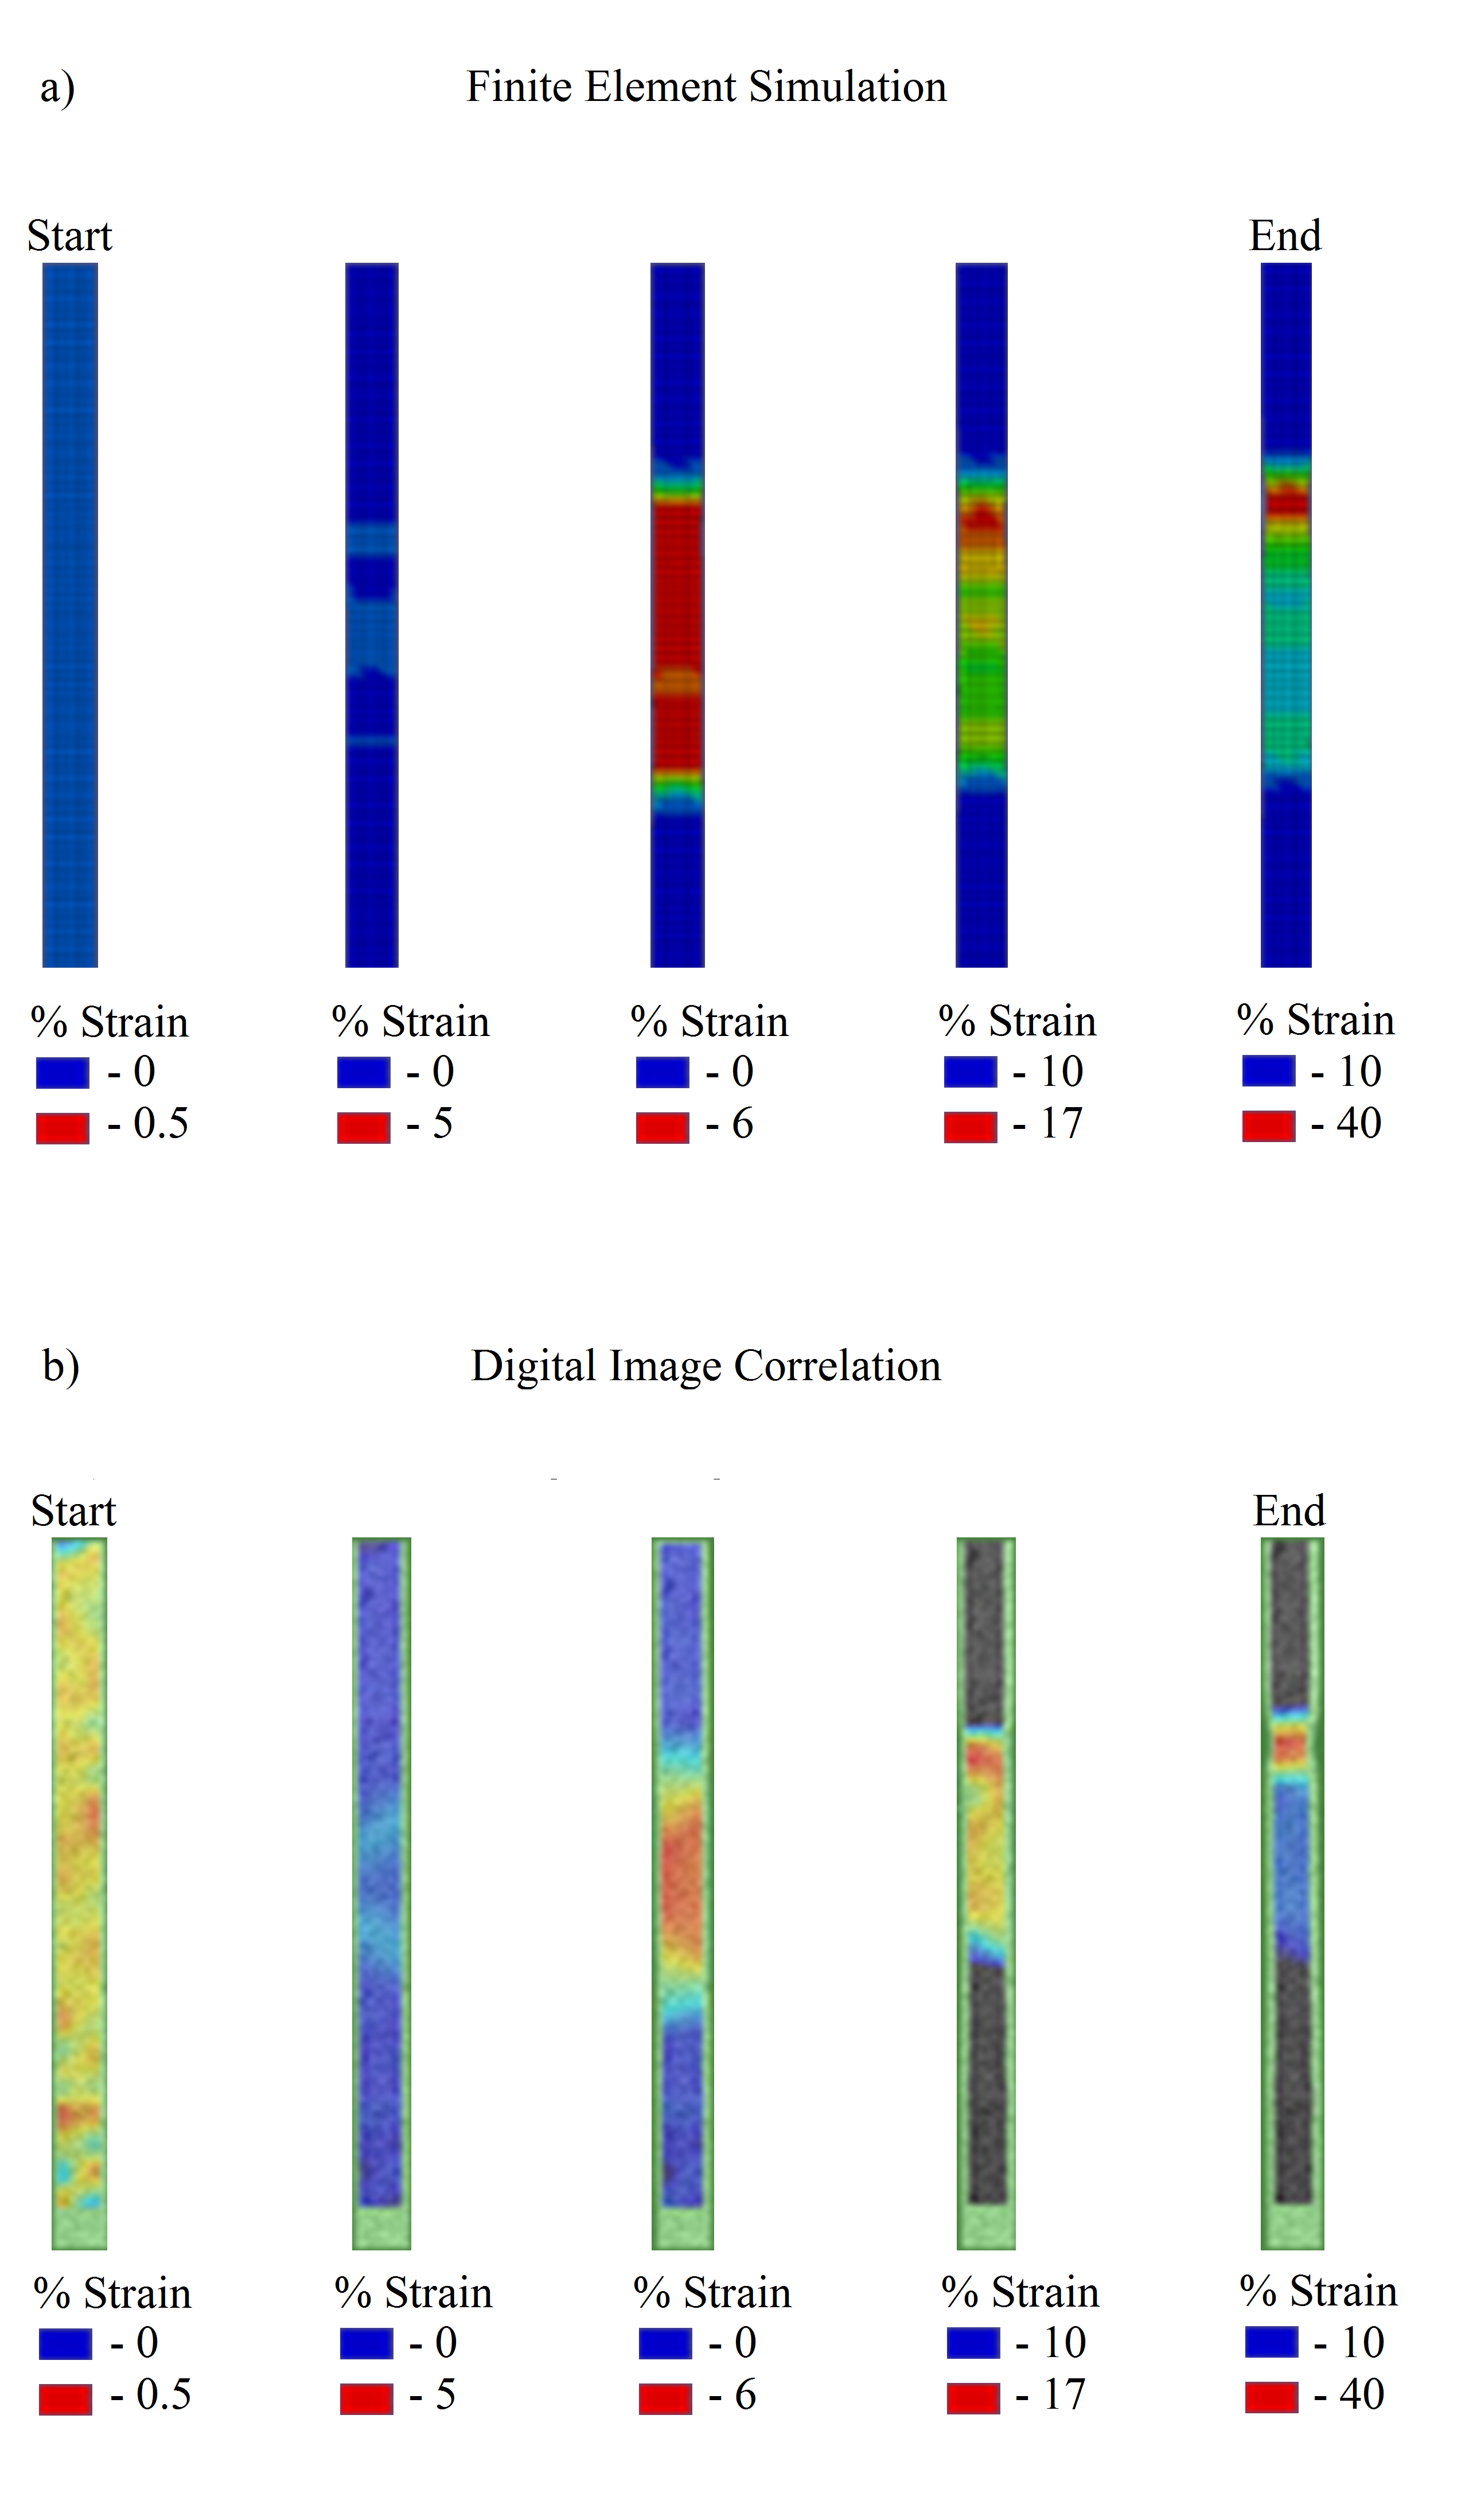
\includegraphics[width=1\linewidth]{MacroStrainPredict2}		
%	\caption[Mesh]{a) Predicted strain evolution using method in \S\ref{FE}. b) Experimentally measured strain evolution using method in \S\ref{EMDIC}. In both figures, the cross-weld (\textit{x}-direction) strain is plotted}
%	\label{fig:UniaxialStrainMacro}	
%\end{figure} 
%%Figure \ref{fig:UniaxialStrainPredicted} shows the cross weld (\textit{x}-direction) distribution of strain at mid thickness of the weld cross section; this is hereby referred to as axial strain. 
%On a more local scale, figure \ref{fig:UniaxialStrainPredicted} shows the distribution of axial strain at mid thickness of the weld cross section. The figure shows how strain evolves through time as strain is plotted at set global deformation steps (0.1 mm global displacement between the ends of the sample). The evolution through time is illustrated by the transition of colour from blue, at the start of the test, to red, at the end of the test. The figure allows comparison of the predicted strain using the method in \S\ref{FE} and experimentally measured strain using the techniques in \S\ref{EMUniaxialLoading}.
%The experimental evidence shows that during the early stages of deformation, axial strain appears to be distributed across the inner regions of the weld (nugget and TMAZ). Axial strain then increases, and is most prominent, in these innermost regions of the weld zone but also occurs in the HAZ. All of the axial strain does, however, appear to be confined to the weld zone, or the region defined by the width of the HAZ. Axial strain continues to increase until a critical point, with respect to global deformation of the sample, when it begins to localise (approximately -12 mm from the weld centreline) within the weld zone. The axial strain is distributed uniformly within the inner regions of the weld and measures approximately 15\%. As the strain localises in the weld zone, it rapidly increases to approximately 22\% before failure. 
%In line with experimental evidence, the prediction using the method in \S\ref{FE} shows that axial strain is distributed across the inner regions of the weld during the early stages of deformation, and is greatest in the nugget. Strain increases across the weld, as the sample is loaded, but remains confined within the weld zone. Axial strain continues to increase until a critical point, with respect to global deformation, when it begins to localise approximately -12 mm from the weld centreline. Axial strain varies between 10-15\% across the inner regions of the weld but remains stable, whilst localisation causes a rapid increase in strain towards the end of the simulation. The predicted geometric distribution of strain through deformation appears to correlate closely with experimentally measured results. In addition, the position of strain localisation is predicted accurately. 
%
%Upon examination of the variation initial flow stress across the weld (see figure \ref{fig:colormaps}), it is clear that initial deformation will occur in the nugget region since this region has the lowest flow stress. 
%This is in line with materials data on FSW 2139-T8 reported by Gruijicic \cite{Grujicic2011a}, though data from McWilliams \cite{McWilliams2013} shows that the TMAZ in 2139-T8 welds can exhibit the lowest initial flow stress. However, the reported weld conditions together with micrographs indicate that the thermal cycles in those welds were quite low \cite{Mishra2005}. It is possible that the overall variation in strengthening mechanisms in these studies are different to those described in Part II. Deformation behaviour of 2024 alloy, as reported by Genevois \cite{Genevois2006} and Sato \cite{Sato1999,Sato2001,Sato2001b}, also shows initial yielding in the nugget region and the contributors to strengthening mechanisms are similar to the conclusions from Part II. Since there is no description of the strengthening mechanisms by McWilliams or Grujicic the cause of initial yielding in their studies is unclear. However, it is possible that the difference is linked to the markedly different welding parameters, and therefore the thermal loading, used in each study \cite{Mishra2005}.
%As the nugget region work hardens, the surrounding region (TMAZ and inner regions of the HAZ) begins to deform since the flow stress is equal to that of the nugget region. Since the nugget region has a greater work hardening rate than the immediate surrounding material \cite{Grujicic2011a,Genevois2006}, strain will not, in theory, localise here except in the presence of some defect. 
%The high work hardening rate of nugget material as compared to material elsewhere in the weld or parent material in age hardened alloys has also been reported by Karlsson \cite{Karlsson2000} and Mahoney \cite{Mahoney1998} and is generally true for peak hardened aluminium alloys subjected to FSW.
%As strain develops it is mainly distributed across the inner regions of the weld zone until a critical point where it localises just outside the position of minimum hardness of the weld; the hardness minima represents the boundary between the inner and outer HAZ, as shown in Part II. However, this is not generally true and depends on the initial aging condition. Further, some 7xxx alloys, for example, have several kinds of second phase precipitate which contribute to strengthening \cite{Sullivan2011}. Each precipitate may respond differently to the thermal cycle and it is not necessarily the case that the hardness minima and strengthening mechanism variation are correlated. Strain begins to localise when the inner regions of the weld have work hardened to a point where the flow stress is equal to or greater than the minimum flow stress of the outer HAZ (the boundary of the inner and outer HAZ). Combined with the gradient in flow stress in the outer region of the HAZ, which forces strain localisation towards the centre of the weld, since the work hardening rate of the inner regions of the weld is much greater than the outer HAZ, strain should theoretically begin to localises just outside the hardness minima. 
%
%In 2139-T8 alloy, from the results presented in Part II, the changes in strain rate across the weld are linked to the variation in strengthening mechanism induced by the welding process. The parent material has low work hardening rate due to high dislocation density from processing and the dominance of the $\Omega$ strengthening phase. The outer HAZ has similar work hardening rate because, even though dislocation density is reduced (through dislocation annihilation processes arising from thermal loading) and $\Omega$ phase is coarser and less finely distributed than the parent phase having overaged from the T8 condition \cite{Grujicic2010}, the dominant strengthening mechanism is still the same as the parent material. In the inner regions of the HAZ, TMAZ, and nugget the temperatures are high enough to cause dissolution of $\Omega$ on a local scale and further annihilate dislocations; the precise location where this occurs coincides with the hardness minima in the weld cross section. Hence, in these inner regions, contribution from strengthening mechanisms such as solid solution strengthening and the formation of Guinier-Peston (GP) zones after natural aging become important \cite{Grujicic2010,Cho2006,Bakavos2008}. $\Omega$ phase does not re-precipitate out because there is no controlled heat treatment process after the welding proces. Whilst grains in the TMAZ have undergone severe plastic deformation, they are still of the same order of magnitude as the parent material and outer HAZ. However, grains of the nugget have undergone dynamic recrystallisation due to the combination of thermal loading and plastic deformation. The effect of grain size refinement becomes an additional contributor to strengthening mechanism in this region \cite{Sato1999,Sato2001b}. Therefore, if we consider the distribution of material properties in figure \ref{fig:colormaps}, the distinct changes work hardening rate are physically reasonable. Indeed, the smooth gradient in flow stress up to the location of the hardness minima, and the uniform distribution of flow stress in the inner regions of the HAZ which only change within the nugget are also physically reasonable. 
%
%It is clear that the accurate description of material properties, which is linked to the variation in strengthening mechanism in the welded alloy, has facilitated the prediction of the evolution of strain distribution in the weld. Whilst no attempt is made to determine failure in the model, it is clear that using the \S\ref{FE} modelling approach, the precise location of strain localisation can be determined and the evolution of strain is within order of magnitude and close to experimentally measured evidence. Implementing a failure model linked to strain is likely to match using the presented modelling method.
%%Perfect results in tension. work hardening rate important.
%\begin{figure}[h!]
%	\centering
%	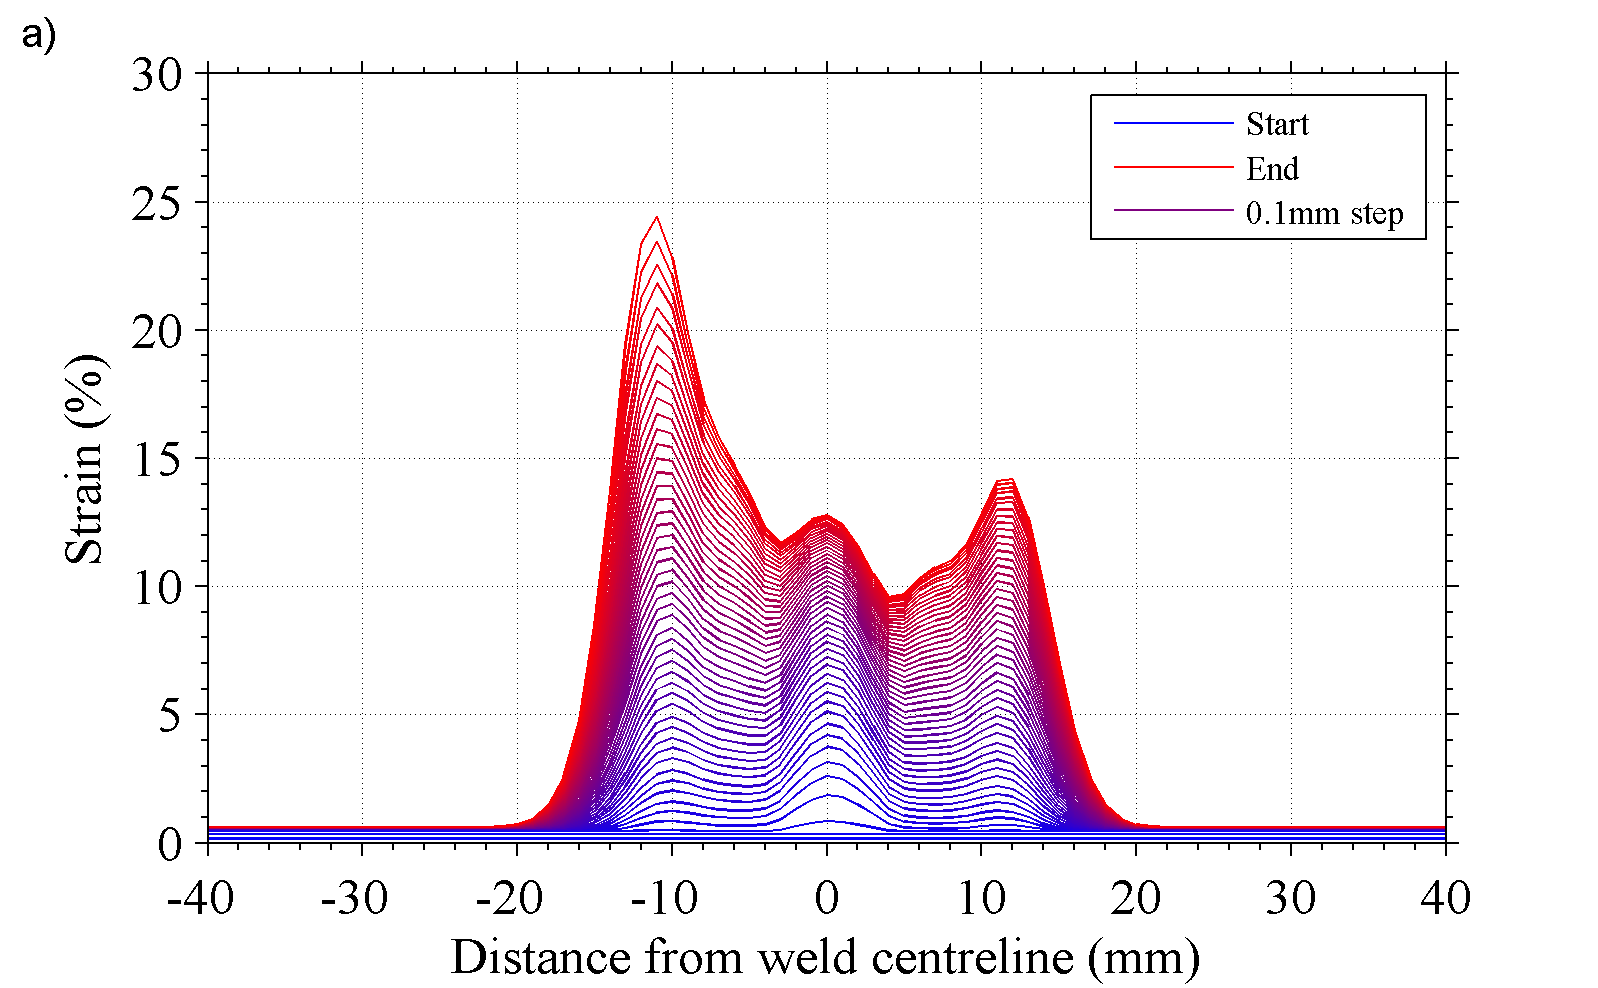
\includegraphics[width=1\linewidth]{PredictedXstrainaltered}		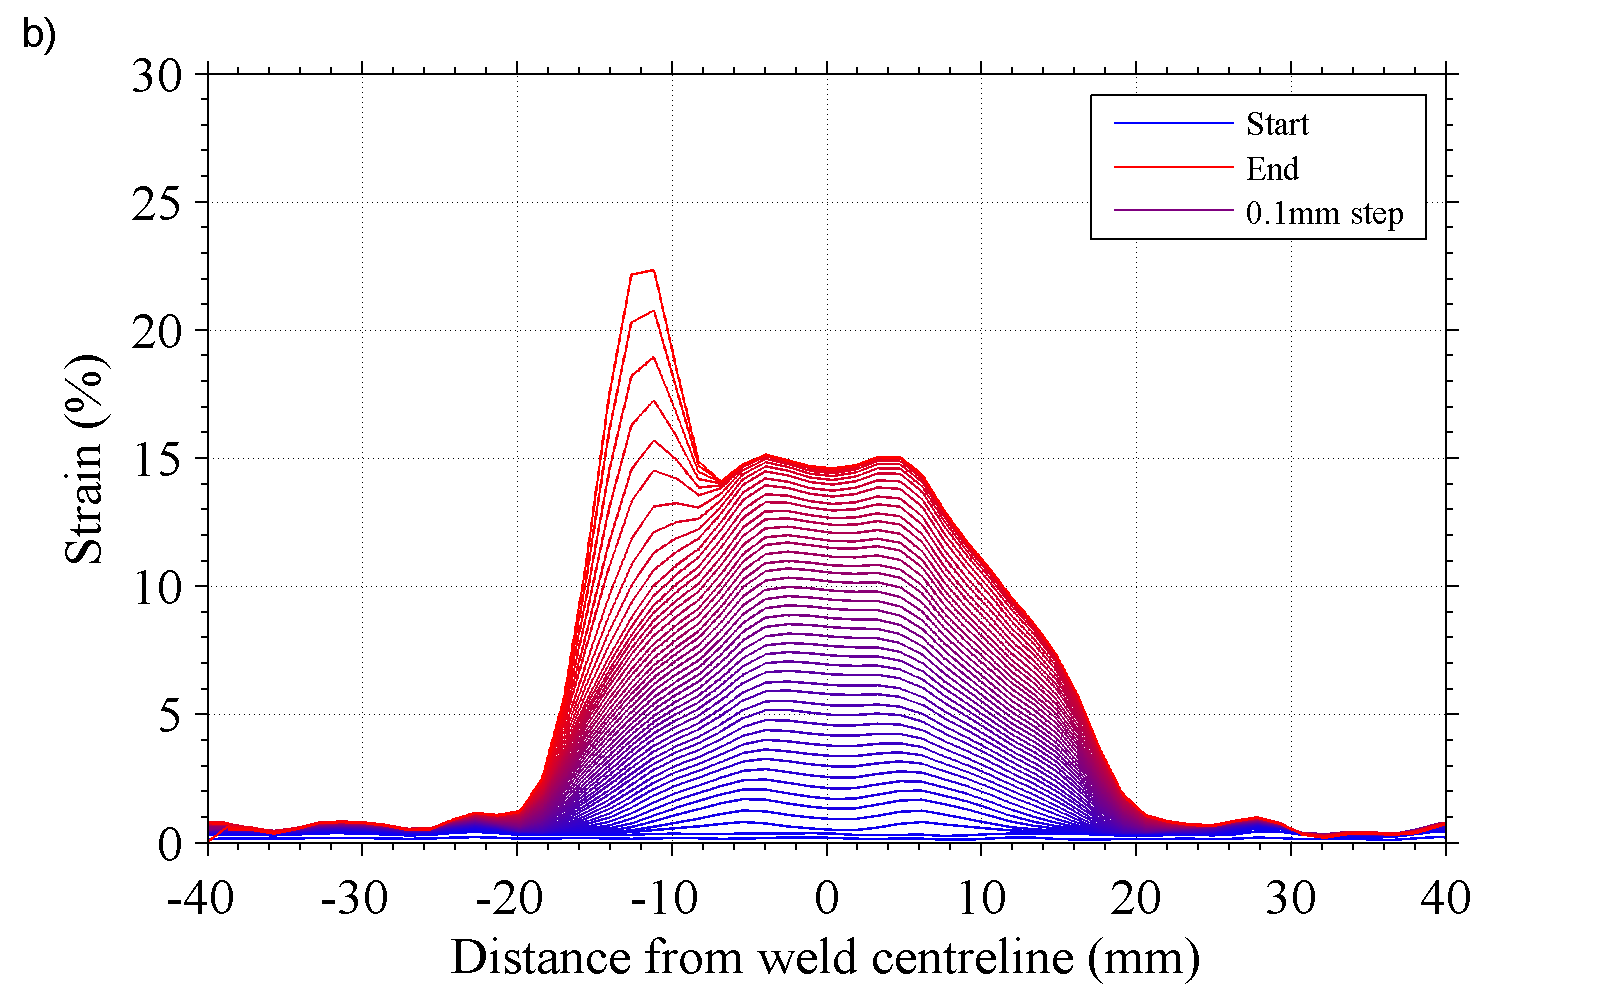
\includegraphics[width=1\linewidth]{DICcrossweldStrainaltered}
%	\caption[Mesh]{a) Predicted strain evolution using method in \S\ref{FE}. b) Experimentally measured strain evolution using method in \S\ref{EMDIC}. In both figures, the cross-weld (\textit{x}-direction) strain is plotted for the mid thickness of the welded plate. In addition, the colour transitions from blue at the start of the test to red at the end of the test; each plot line is for a global displacement between the ends of the sample of 0.1 mm.}
%	\label{fig:UniaxialStrainPredicted}	
%\end{figure} 


\subsubsection{Experimentally measured strain distribution}
\label{SMDModellingstudyResultsExp}
On a macro scale, the evolution of axial strain is illustrated in figure \ref{fig:MacroStrains}a; the associated global stress-strain curve with positions $t_1 - t_5$ is shown in figure \ref{fig:GlobalStressStrain}. It should be noted that there is a discrepancy in the overall measured initial yield stress and the prediction. Initial yielding is assumed to be controlled by the weakest region of the weld, i.e. the TMAZ/nugget. The discrepancy in figure \ref{fig:GlobalStressStrain} is consistent with the observed scatter in nugget data presented in figure \ref{fig:QSWeld}, chapter \ref{ResultsMicrostructure}. 

In the early stages of global deformation, $t_1$, there is a relatively uniform distribution of strain all over the weld cross section. The strain distribution is $\leq 0.5$\% in the \textit{z-x} plane, though there are localised regions of fluctuating strain. At the onset of plastic deformation within the weld, $t_2$, the strain distribution begins to localise in the TMAZ, just outside the nugget region. The strain distribution is approximately symmetrical about the \textit{y-z} plane and peak axial strain measures $\leq 5$\% strain in the \textit{z-x} plane. As global deformation continues, at $t_3$, axial strain remains approximately symmetrical about the \textit{y-z} plane but is predominantly accommodated within the inner regions of the weld, i.e. the inner HAZ, TMAZ, and nugget. Axial strain is measured to be increasing towards the centre of the weld and is greatest within the nugget; peak axial strain measures $\leq 6$\% in the \textit{z-x} plane. At the onset of necking, $t_4$, axial strain begins to localise on the advancing side of the weld, approximately at the interface between the inner and outer HAZ. The strain distribution is no longer symmetrical about the \textit{y-z} plane and peak axial strain is measured to be $\leq 17$\%. Just before the point of failure, at $t_5$, axial strain is localised completely within the necked region of the specimen. Overall, the peak axial strain is measured to be $\leq 40$\% in the \textit{z-x} plane. 

On a local scale, the mid thickness axial strain distribution is shown in figure \ref{fig:LumpedMassPredictions}a. During the early stages of deformation, axial strain is measured to be approximately uniform over the entire sample, and is approximately $\leq 1.5$\% between $|x| \leq 40$ mm. As global deformation continues, strain begins to increase over a progressively wider area of the HAZ, TMAZ, and nugget, and is approximately symmetrical about the centreline of the weld; the distribution of axial strain in this region is increasing towards the centre of the weld. This trend continues until a critical moment in global deformation, where strain begins to localise at approximately $x = -12$ mm, on the advancing side of the weld. At the critical point, the strain distribution is approximately symmetrical and is confined within the region defined by $|x| \leq 20$ mm. Axial strain measures 15\% in the region $|x| \leq 6$ mm. Beyond the critical point, the strain distribution remains approximately constant, except at $x = -12$ mm, where it begins to increase to the point of failure. At the end of the test, axial strain at $|x| \geq 20$ mm is $\leq 1.5$\%; axial strain increases rapidly from $x = -20$ mm to a peak of 22\% at $x = -12$ mm; axial strain decreases to a plateau measuring 15\% between $|x| \leq 7$ mm; axial strain decreases between $x = 7$ mm and $x = 20$ mm.

\begin{figure}[!]
	\subfigure[Measured macro strain distribution]{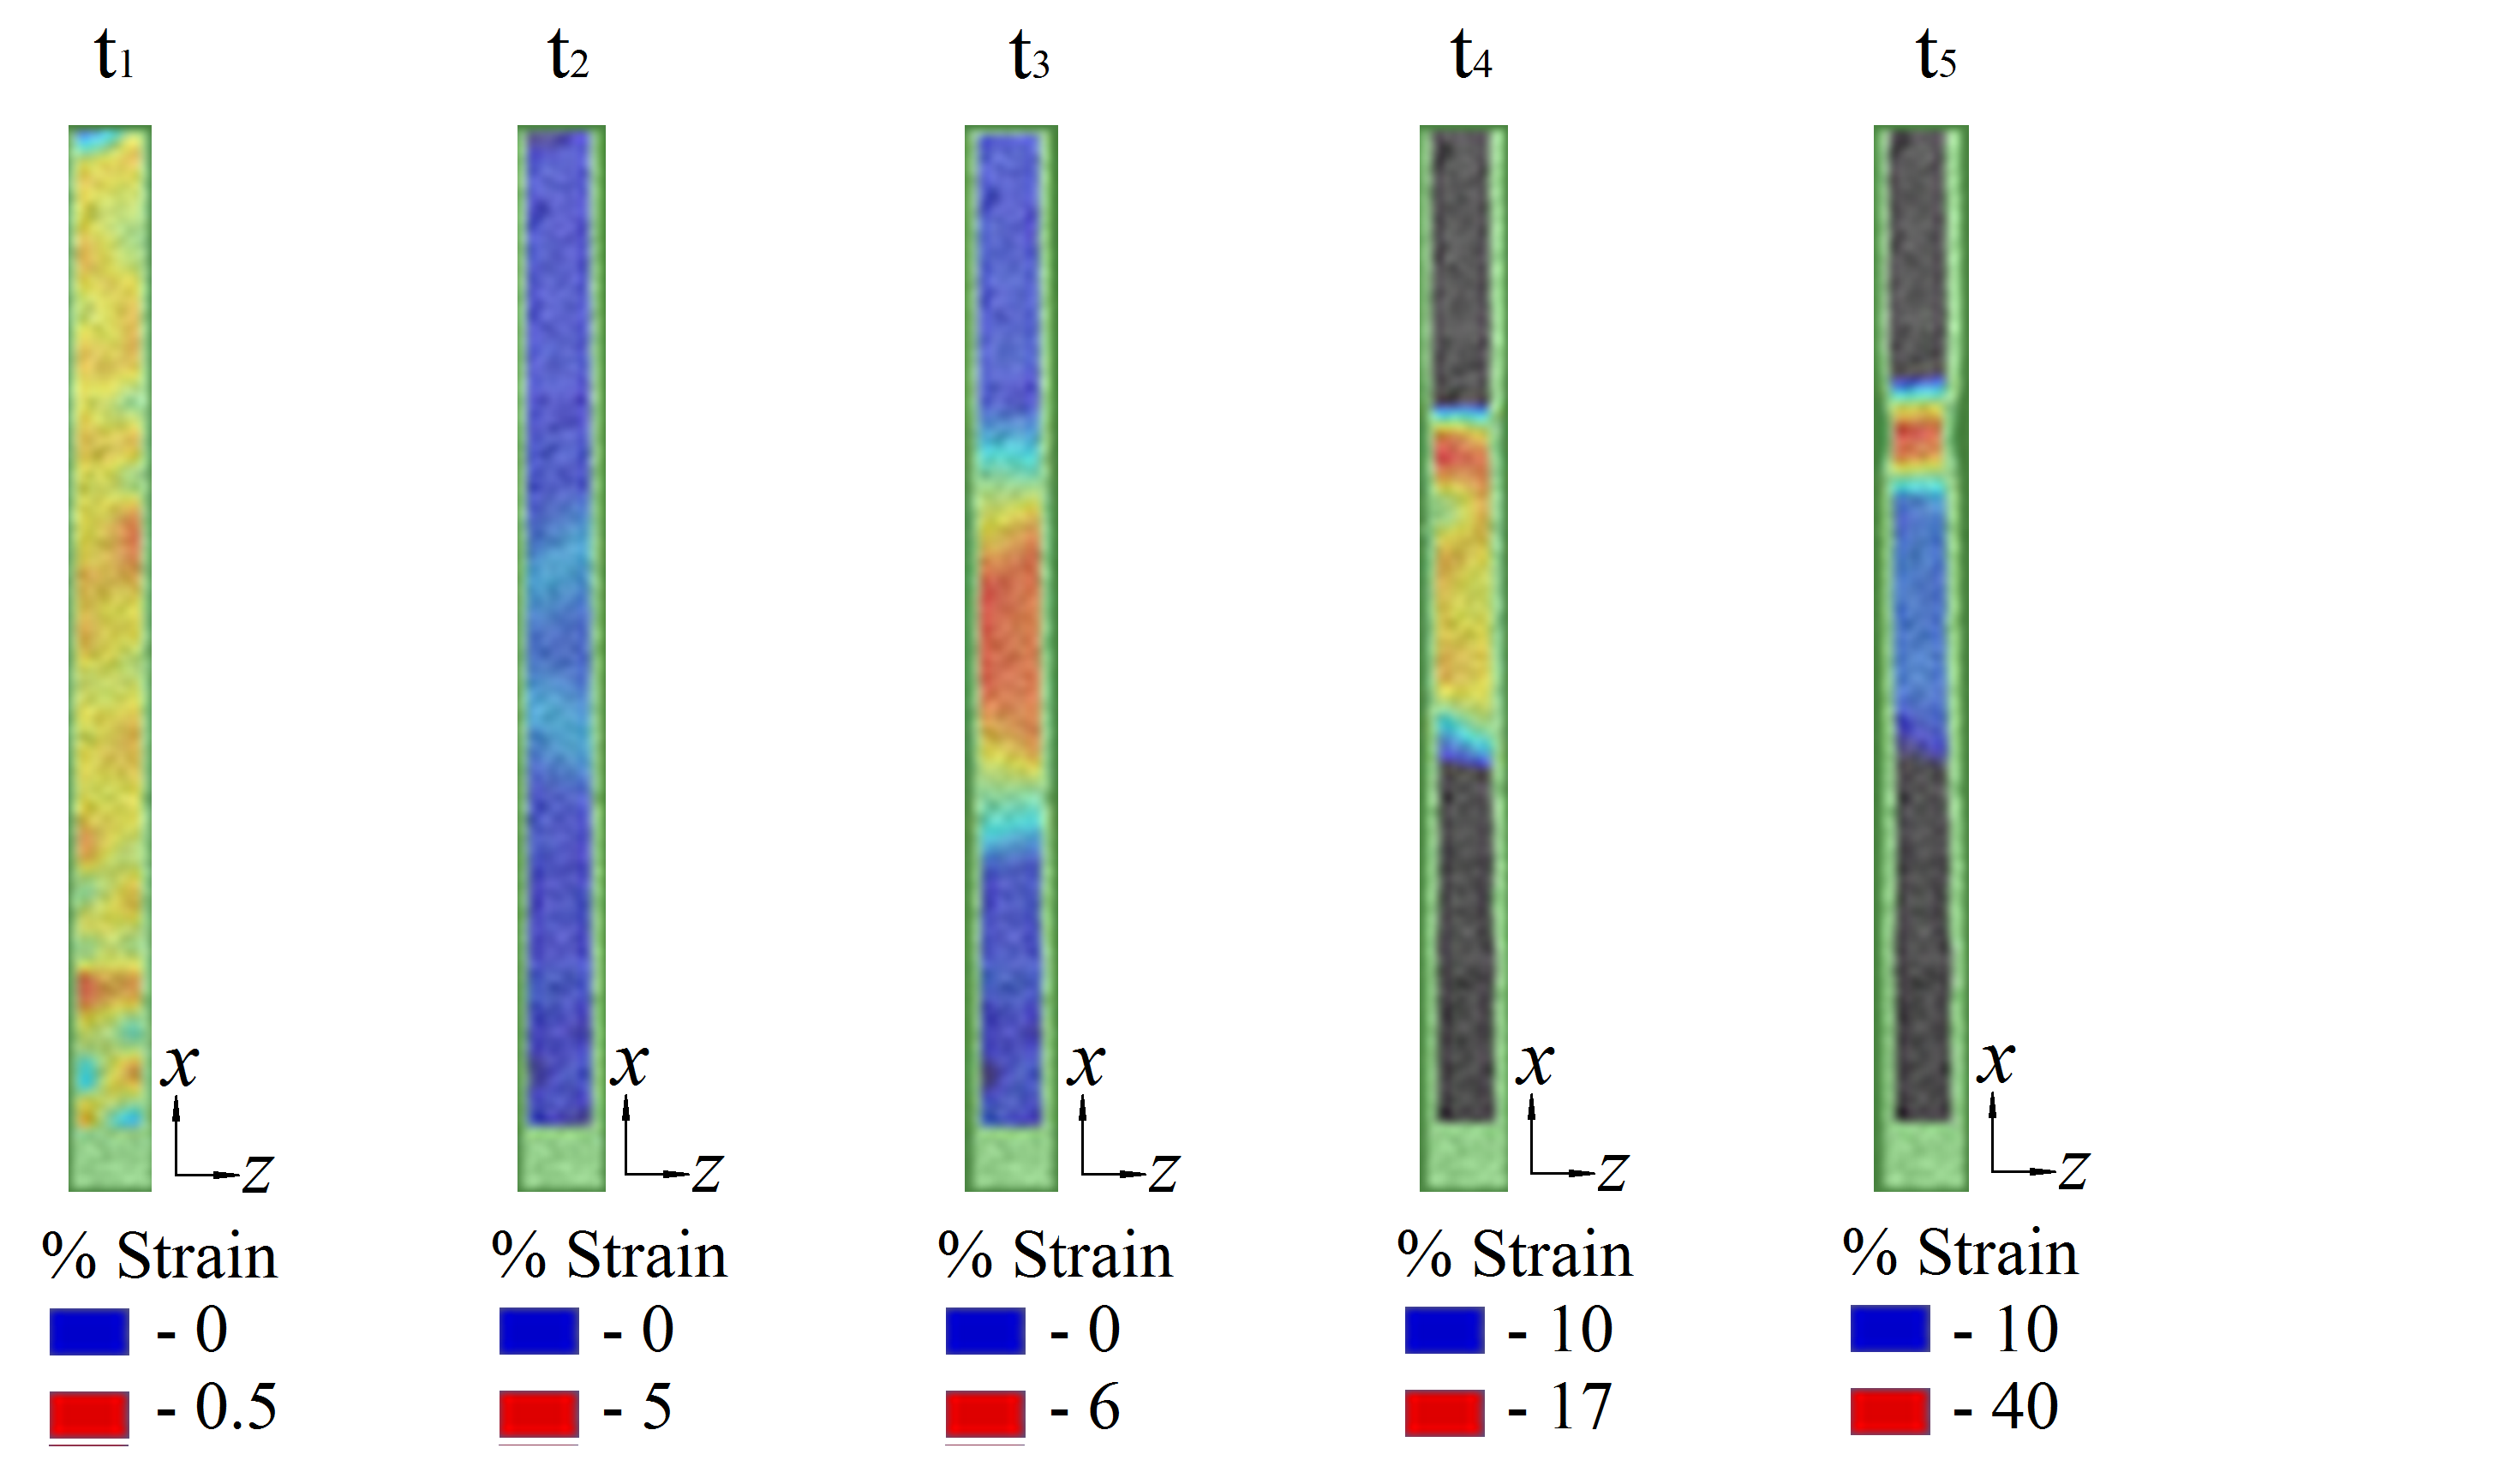
\includegraphics[width=1\columnwidth]{Figures/ModellingMethod/MacroStrainMeasure4}} \centering
	\subfigure[Predicted macro strain distribution]{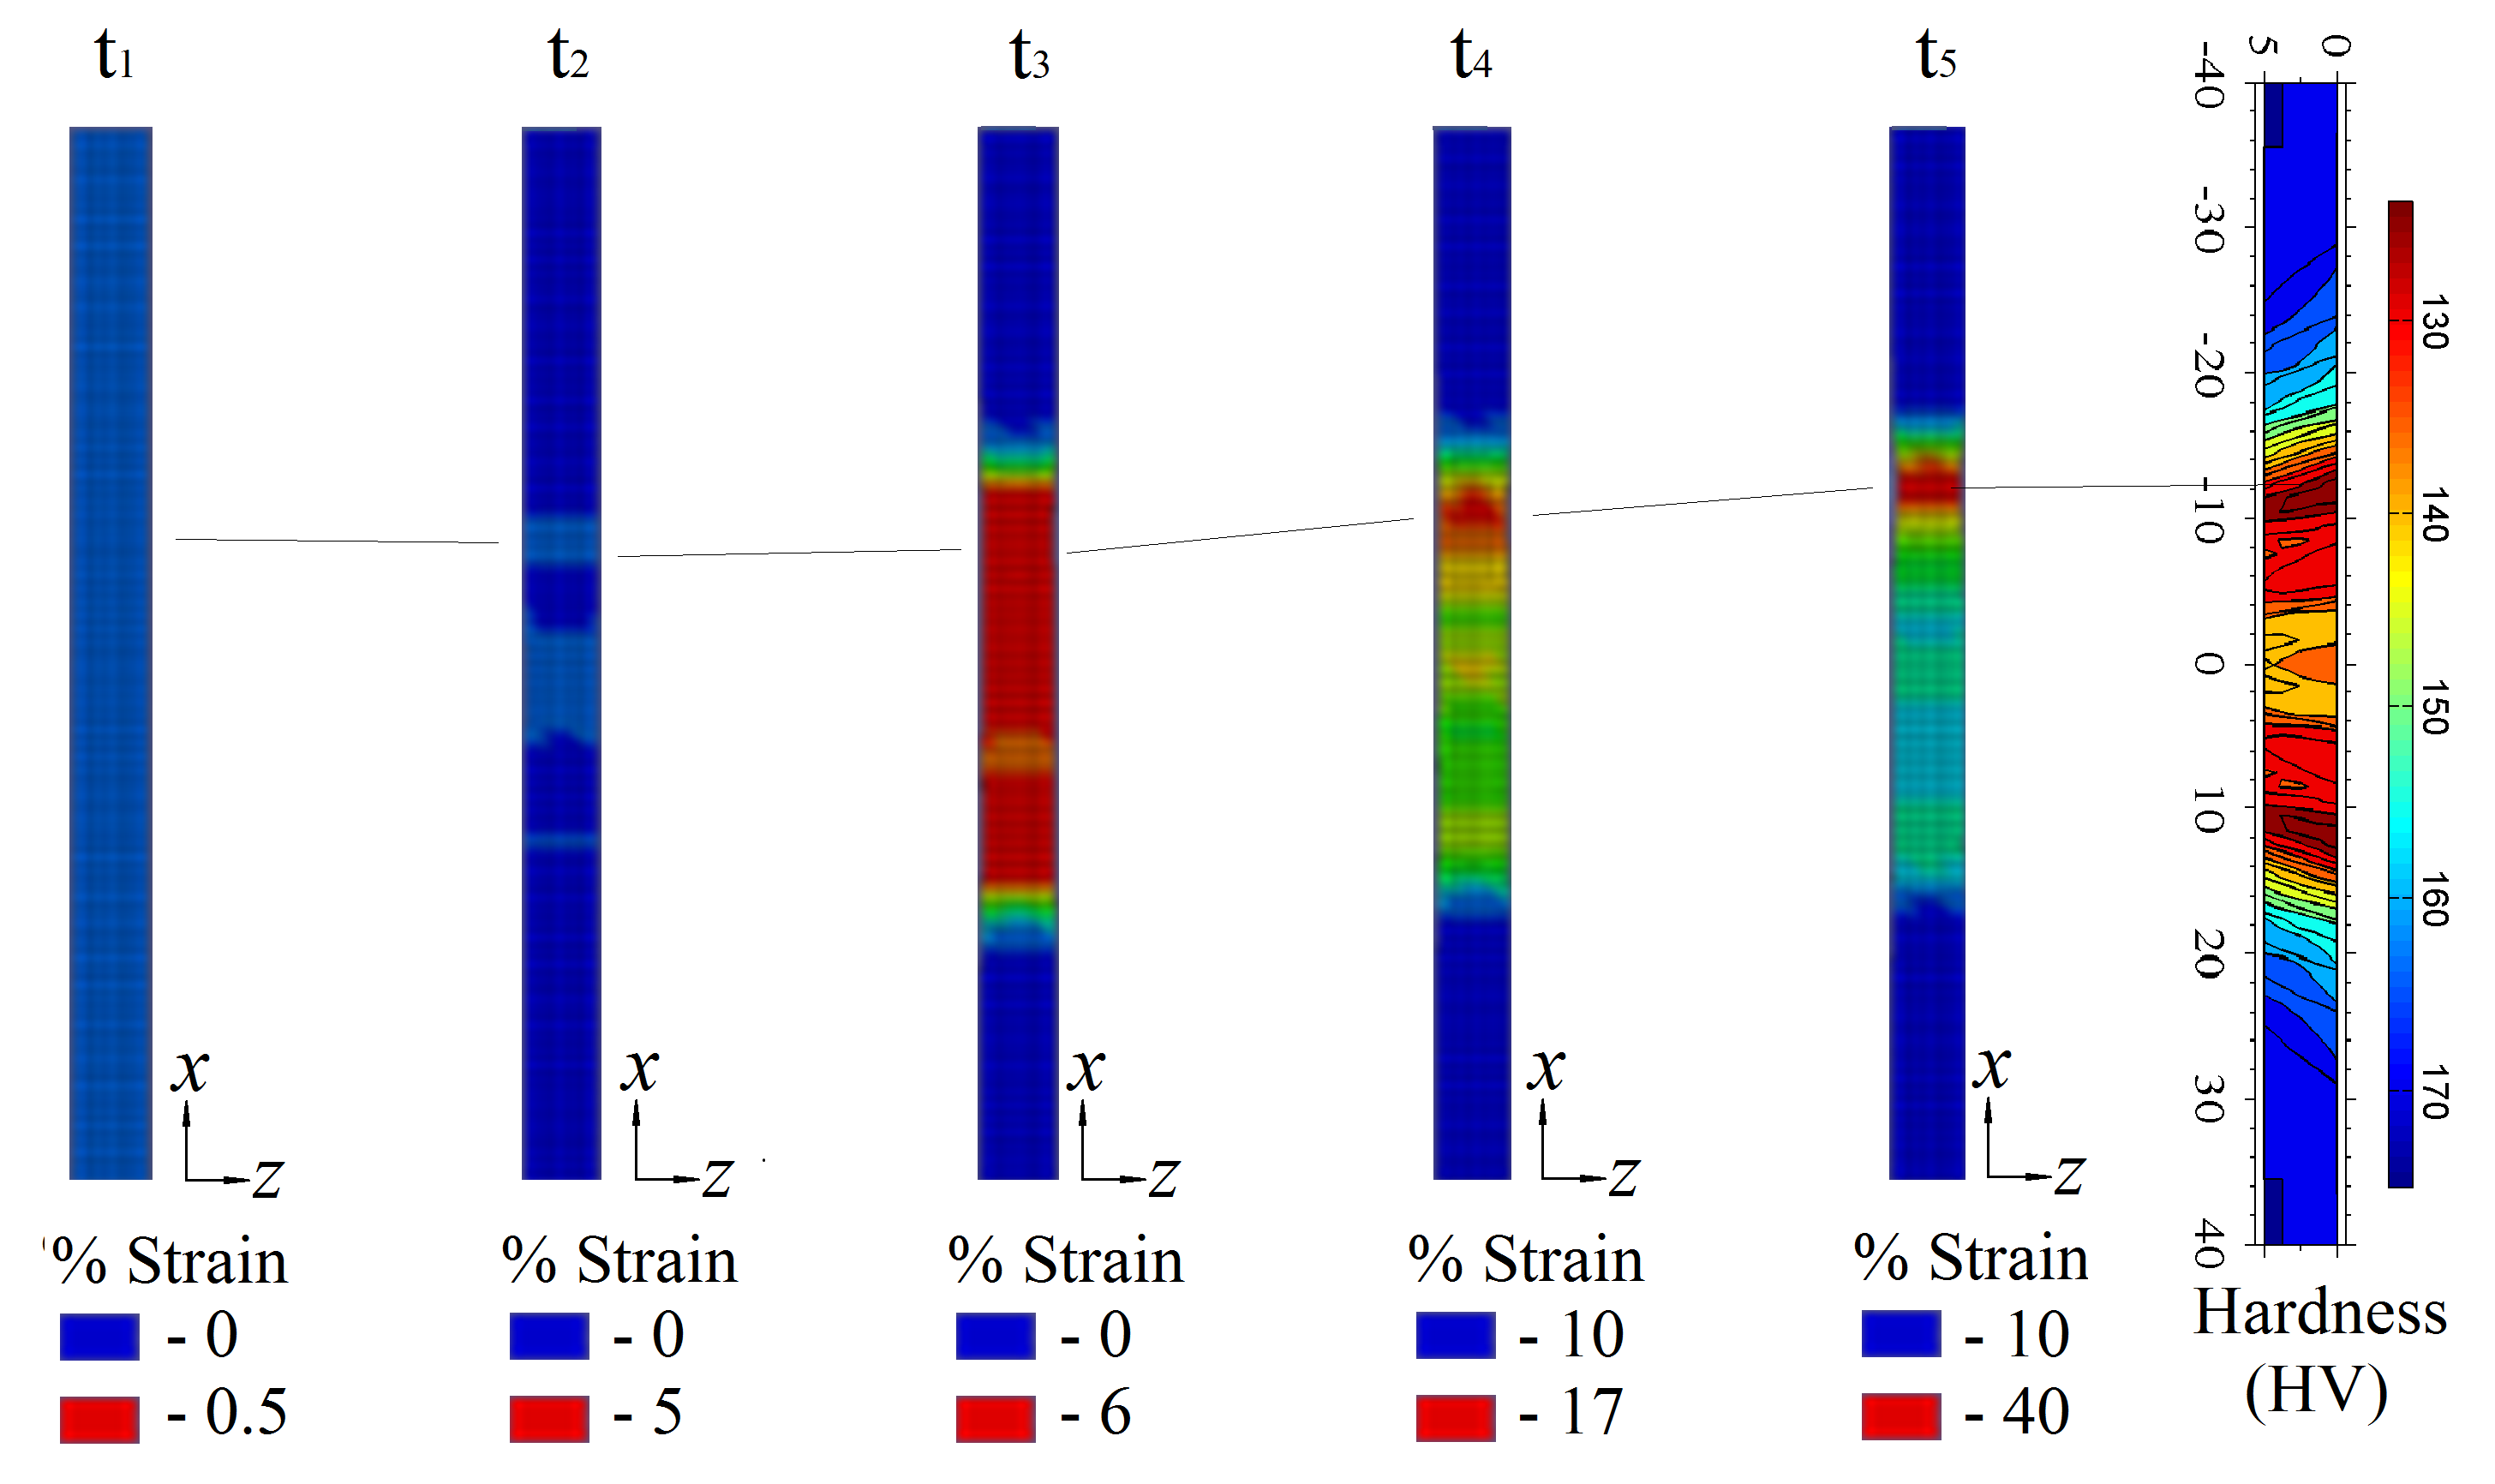
\includegraphics[width=1\columnwidth]{Figures/ModellingMethod/MacroStrainPredict4}} \centering
	\caption[Macro strain distributions]{Macro scale axial strain distribution taken at increasing time steps, transitioning the early stages of deformation to the latter stages of testing. a) Axial strain distribution measured experimentally using DIC. b) Axial strain distribution predicted using optimally defined mechanical property distribution (see details for simulation 9 in table \ref{tab:FEModelInputs}). The time steps equate to the equivalent global deformation steps between the ends of the specimen.}
	\label{fig:MacroStrains}
\end{figure}

\begin{figure}[h!t]
		\centering
		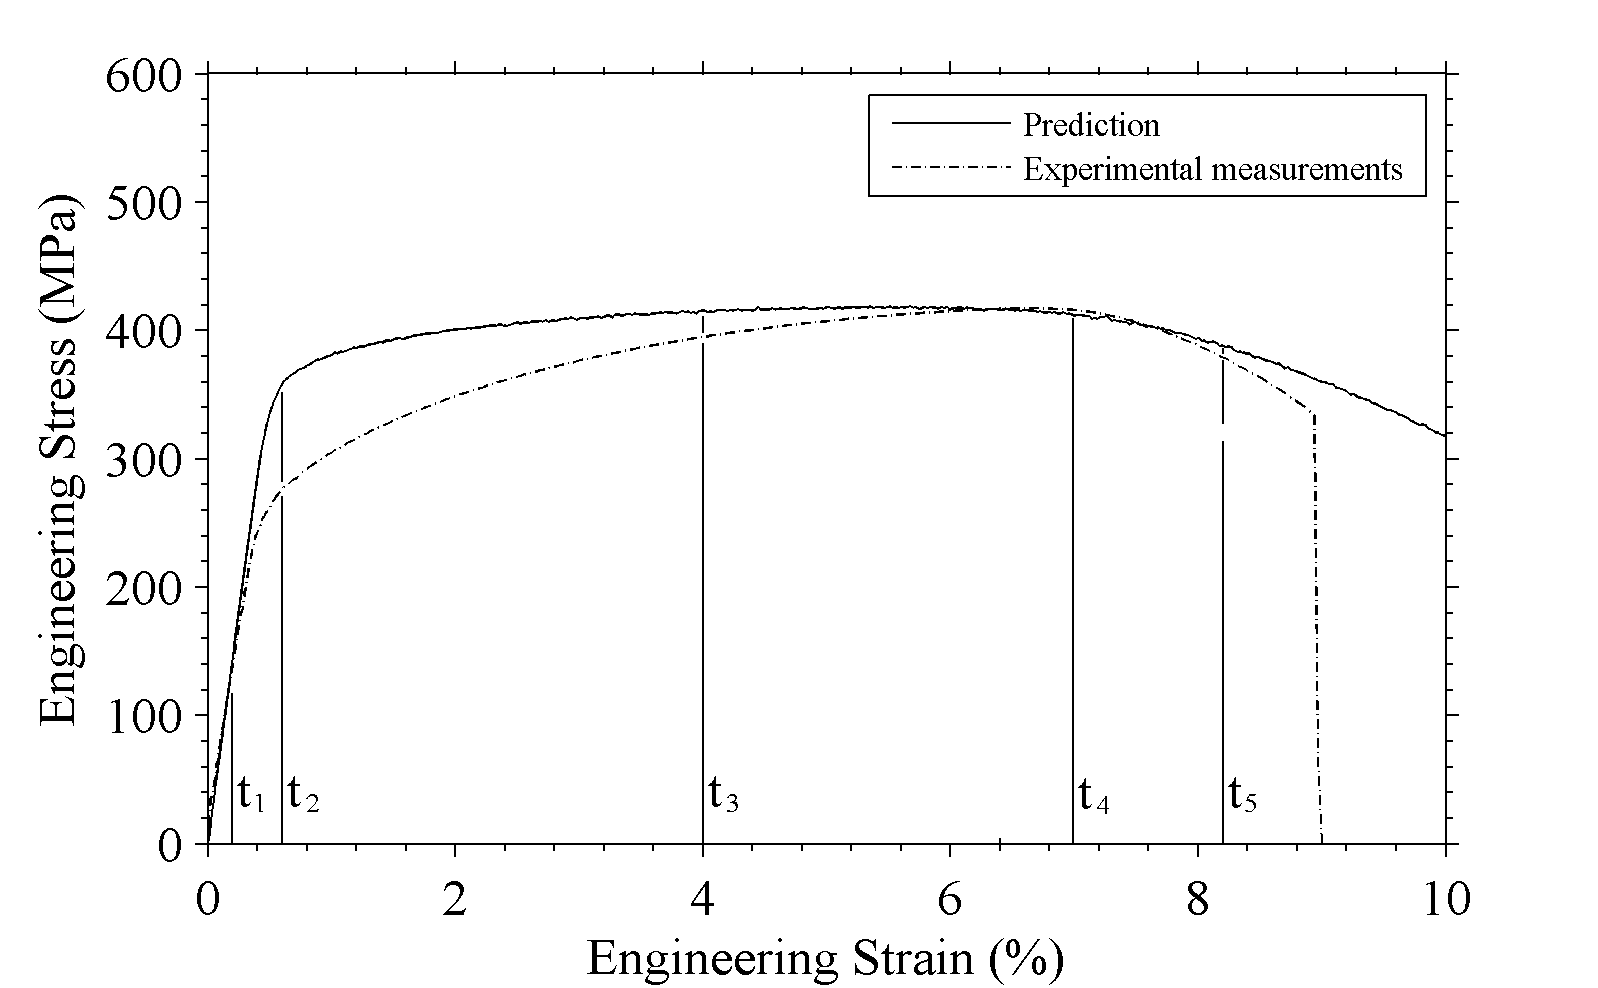
\includegraphics[width=.8\linewidth]{Figures/ModellingMethod/GlobalStressStrainaltered2}
		\caption[Global nominal stress-strain curve]{Predicted and experimentally measured nominal stress-strain curve plotted with the positions $t_1$-$t_5$ marked in figure \ref{fig:MacroStrains}..}
		\label{fig:GlobalStressStrain}
\end{figure}

%\begin{figure}[h!]
%	\subfigure[DIC measured strain]{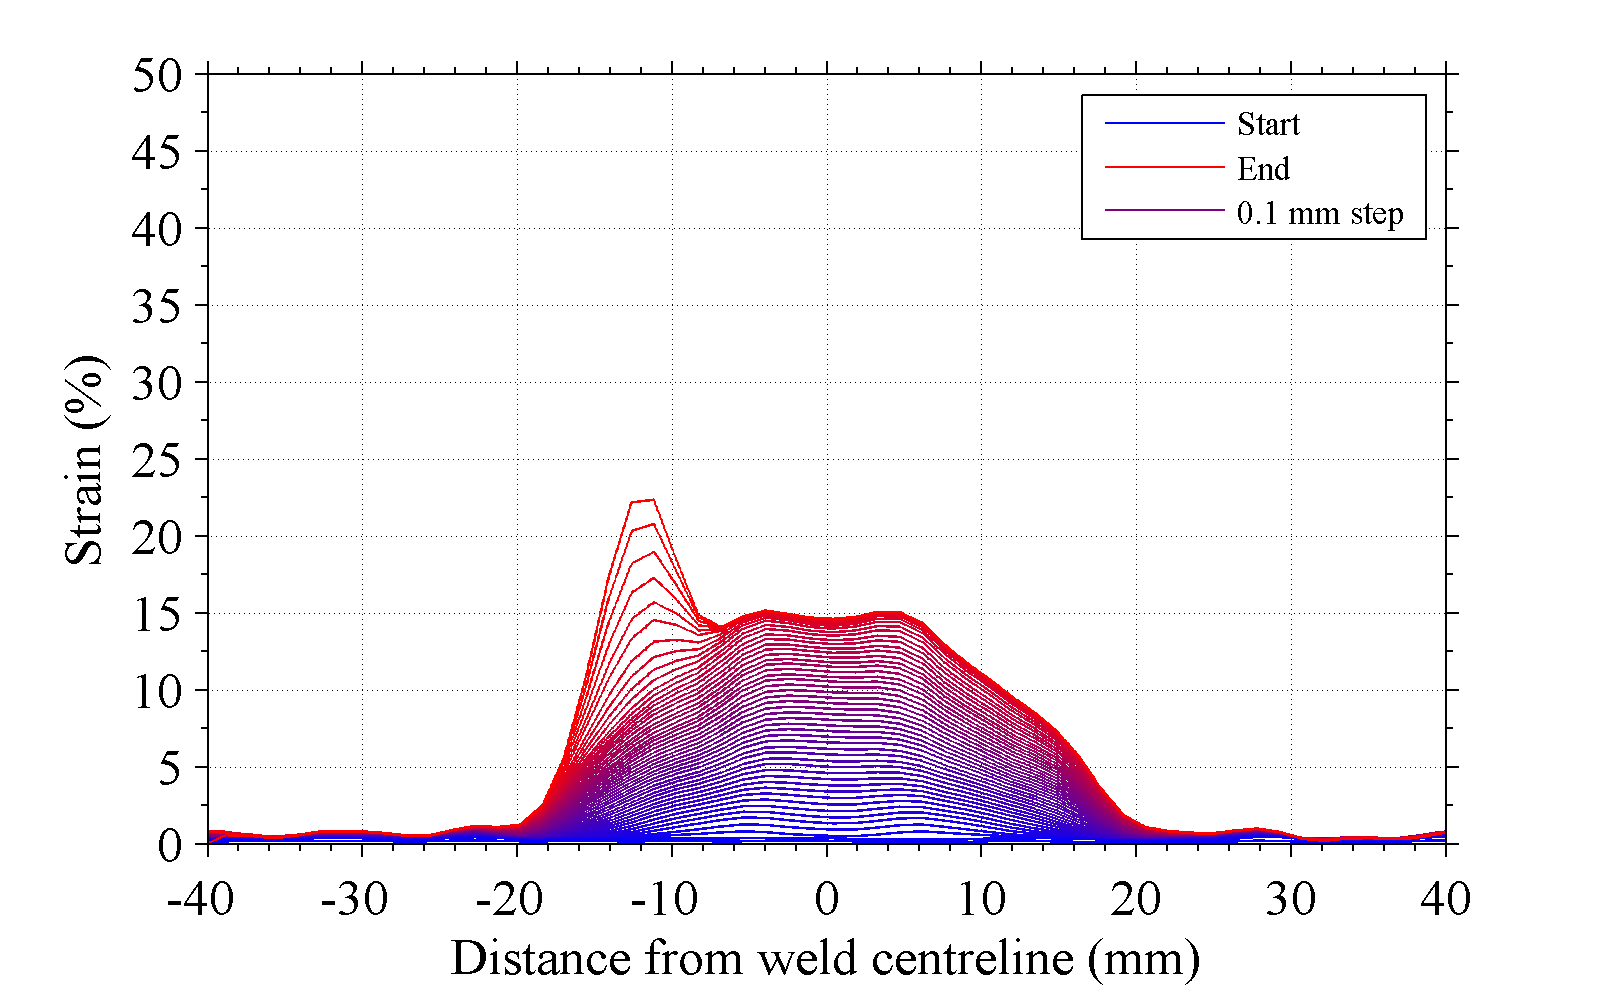
\includegraphics[width=.49\columnwidth]{Figures/ModellingMethod/XStrain_DICMeasuredaltered}}\hfill
%	\subfigure[Optimal inputs: Simulation 9]{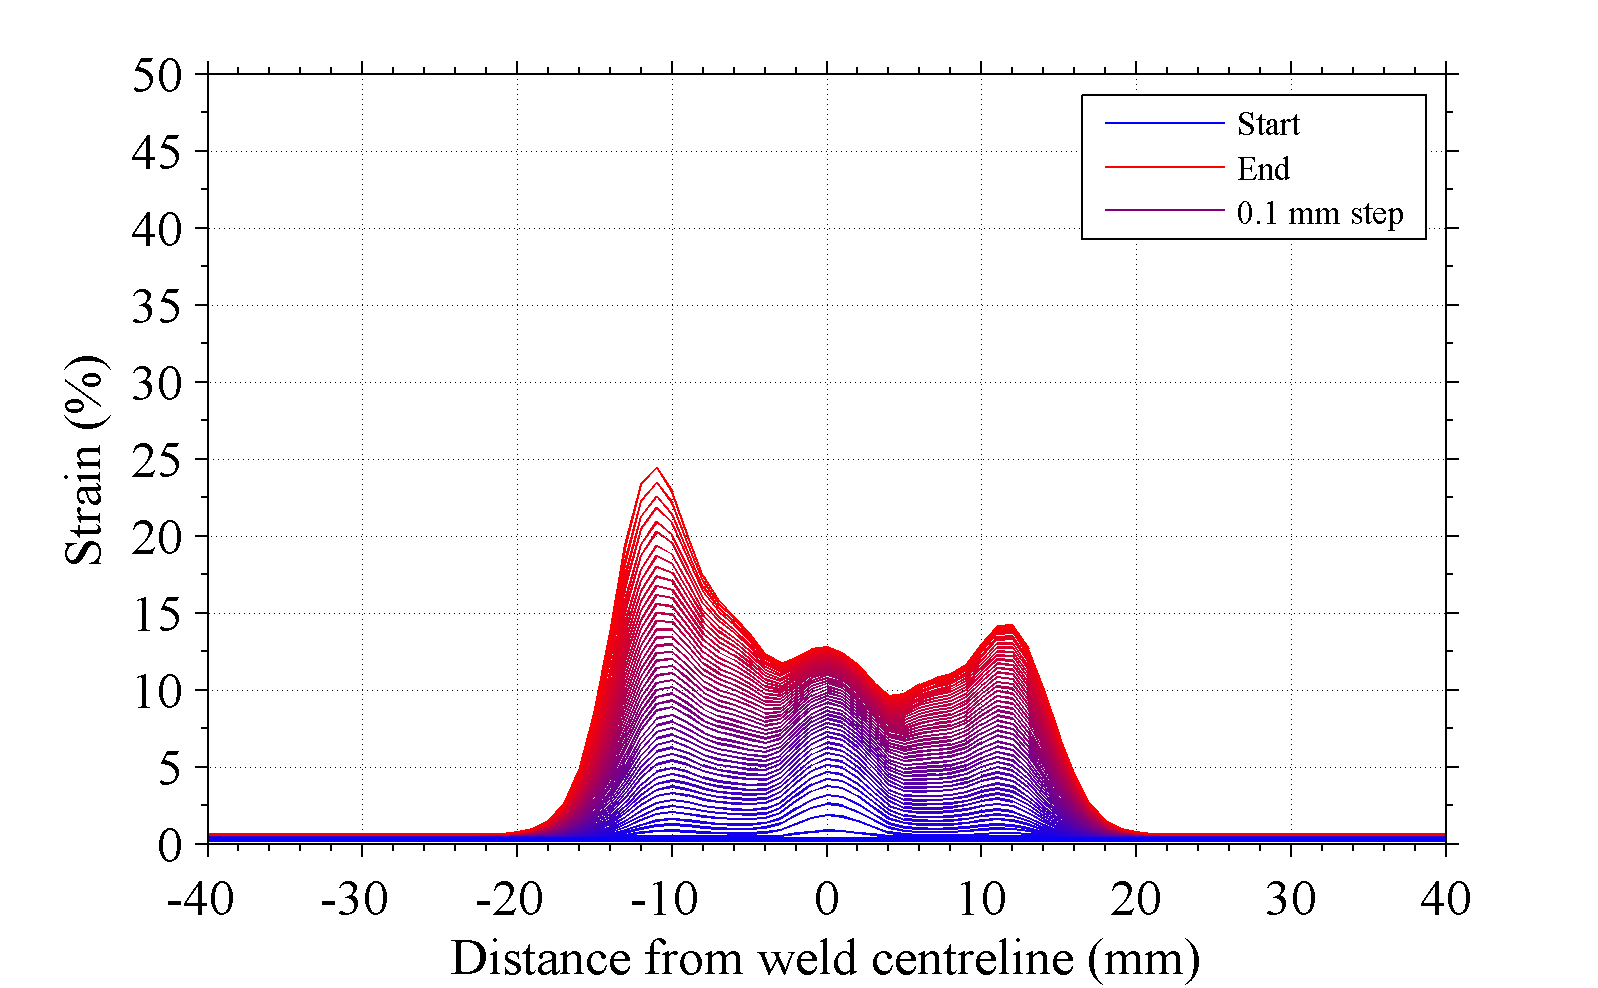
\includegraphics[width=.49\columnwidth]{Figures/ModellingMethod/XStrain_HVSmooth_KStep_NStepaltered}}\hfill
%\caption{Local axial strain distributions for every 0.1 mm global deformation step between the ends of the samples. Measured strain transitions from blue, at the start of the test, to red, at the end of the test.}
%\label{fig:BestStrainDistributions}
%\end{figure}

\subsubsection{Simulations based on the lumped mass method}
\label{SMDModellingstudyResultsSims1to4Correction1}

\begin{figure}[h!t]
	\subfigure[DIC measured strain]{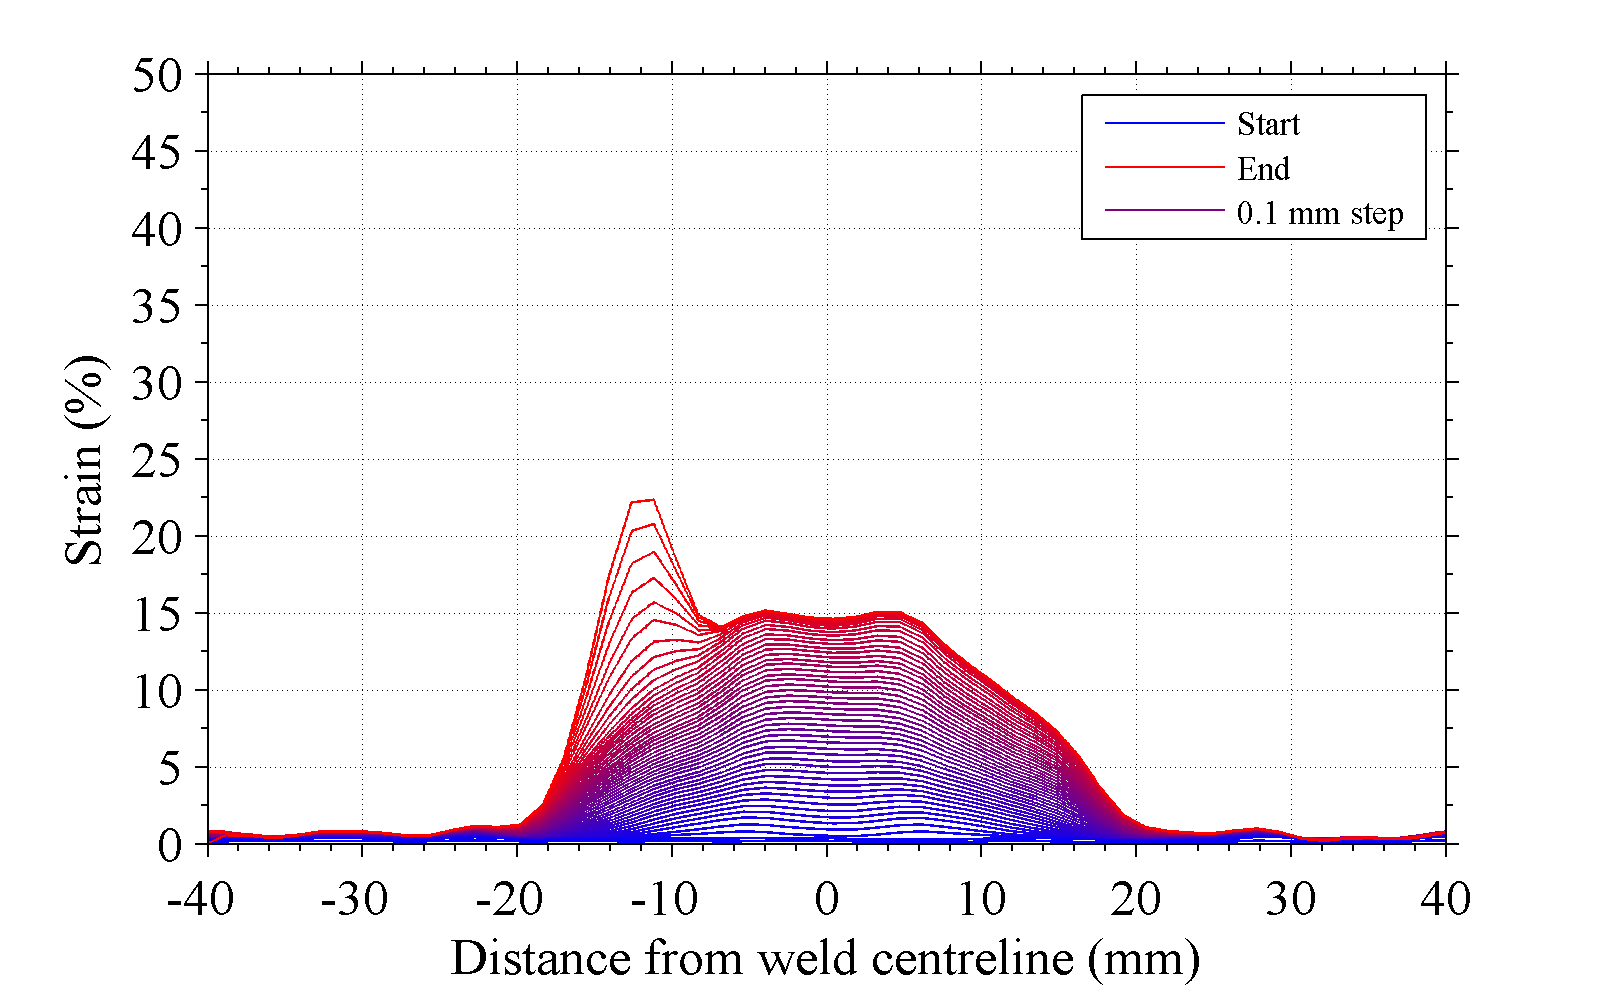
\includegraphics[width=.49\columnwidth]{Figures/ModellingMethod/XStrain_DICMeasuredaltered}}\hfill
	\subfigure[Simulation 1: Hv-step, \textit{k}-constant, \textit{n}-constant]{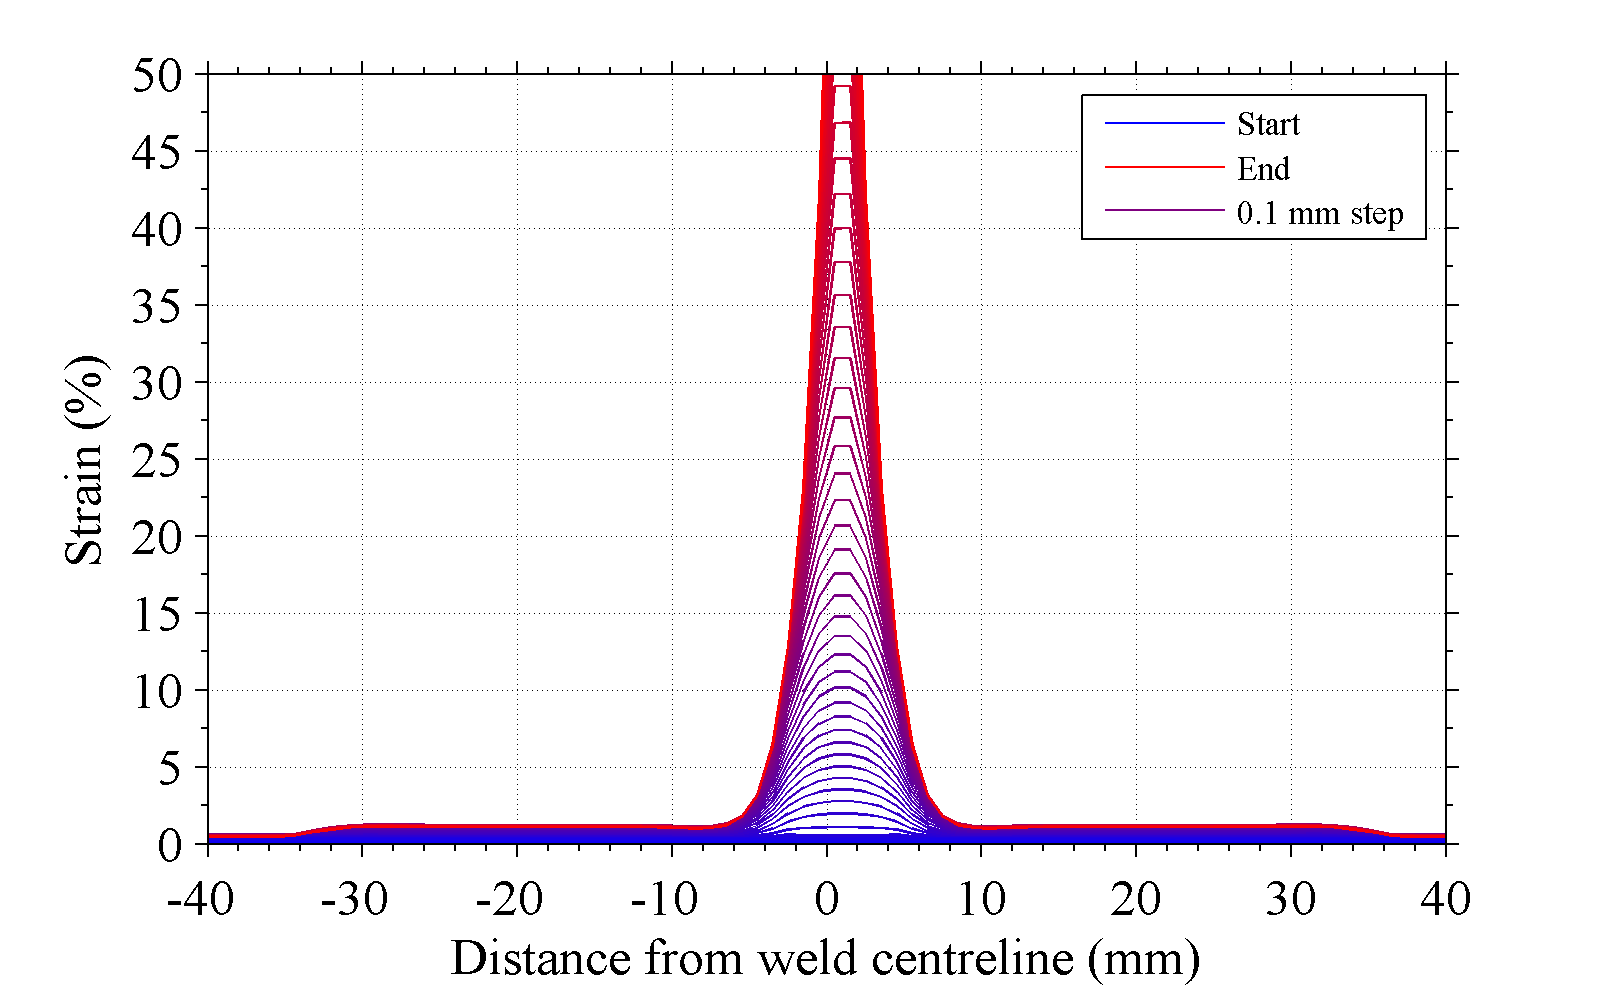
\includegraphics[width=.49\columnwidth]{Figures/ModellingMethod/XStrain_LMDirectaltered}}\hfill
	\subfigure[Simulation 2: Hv-step, \textit{k}-constant, \textit{n}-constant]{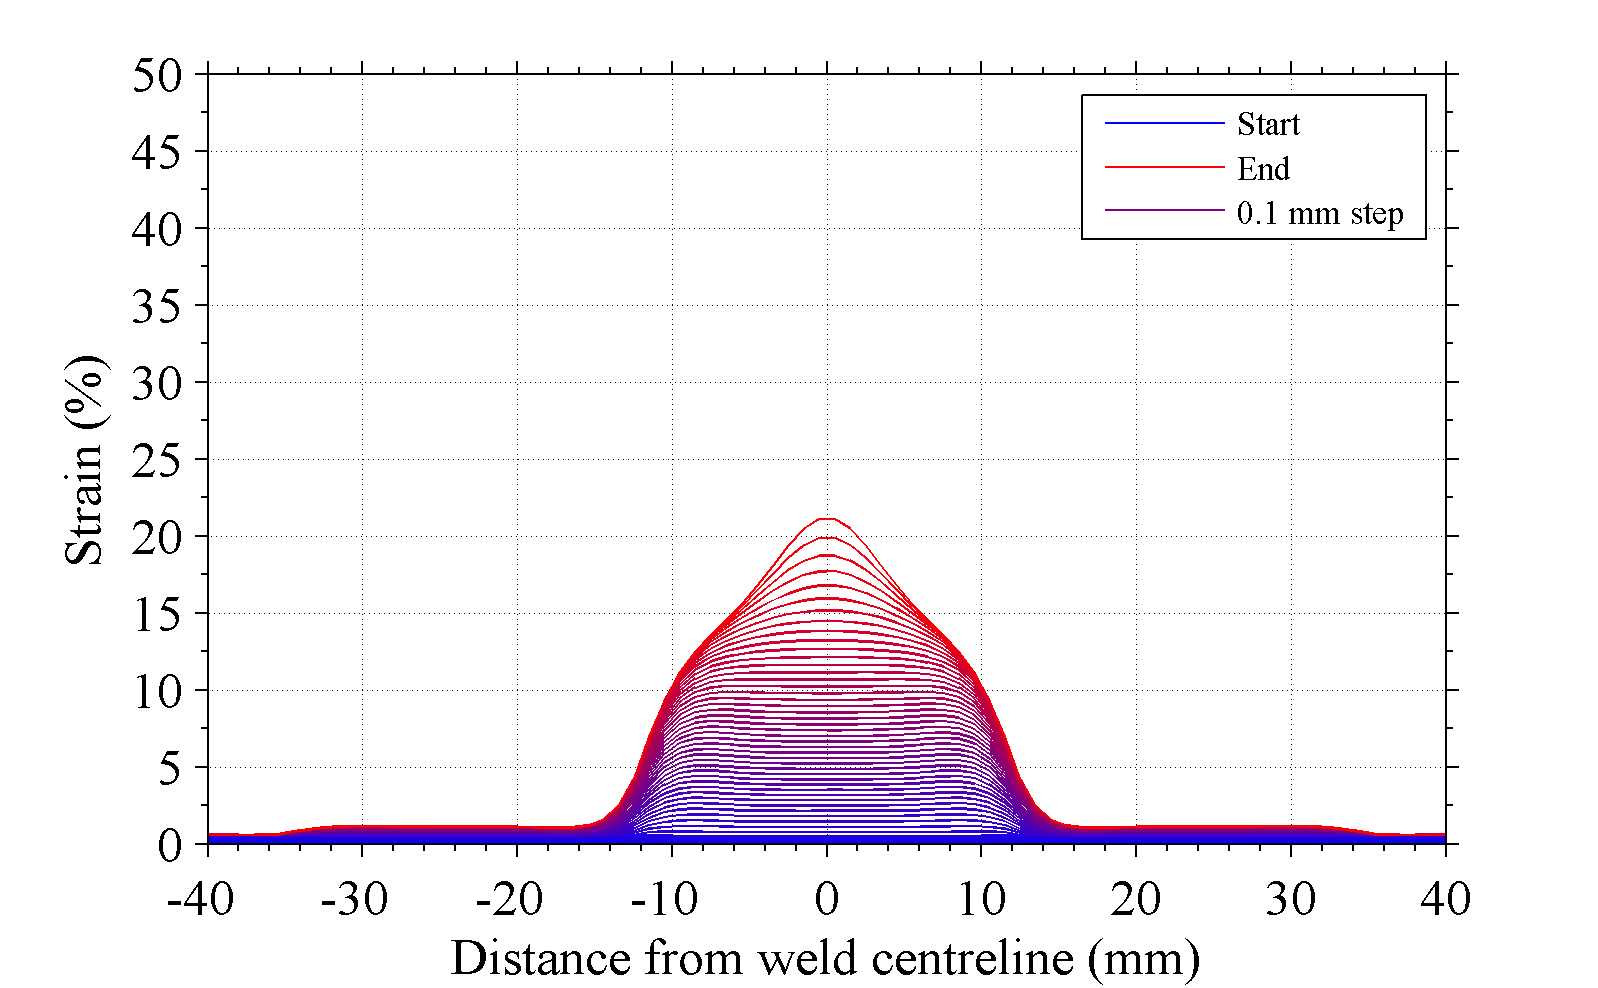
\includegraphics[width=.49\columnwidth]{Figures/ModellingMethod/XStrain_LMCal1altered}}\hfill
	\subfigure[Simulation 3: Hv-step, \textit{k}-constant, \textit{n}-constant]{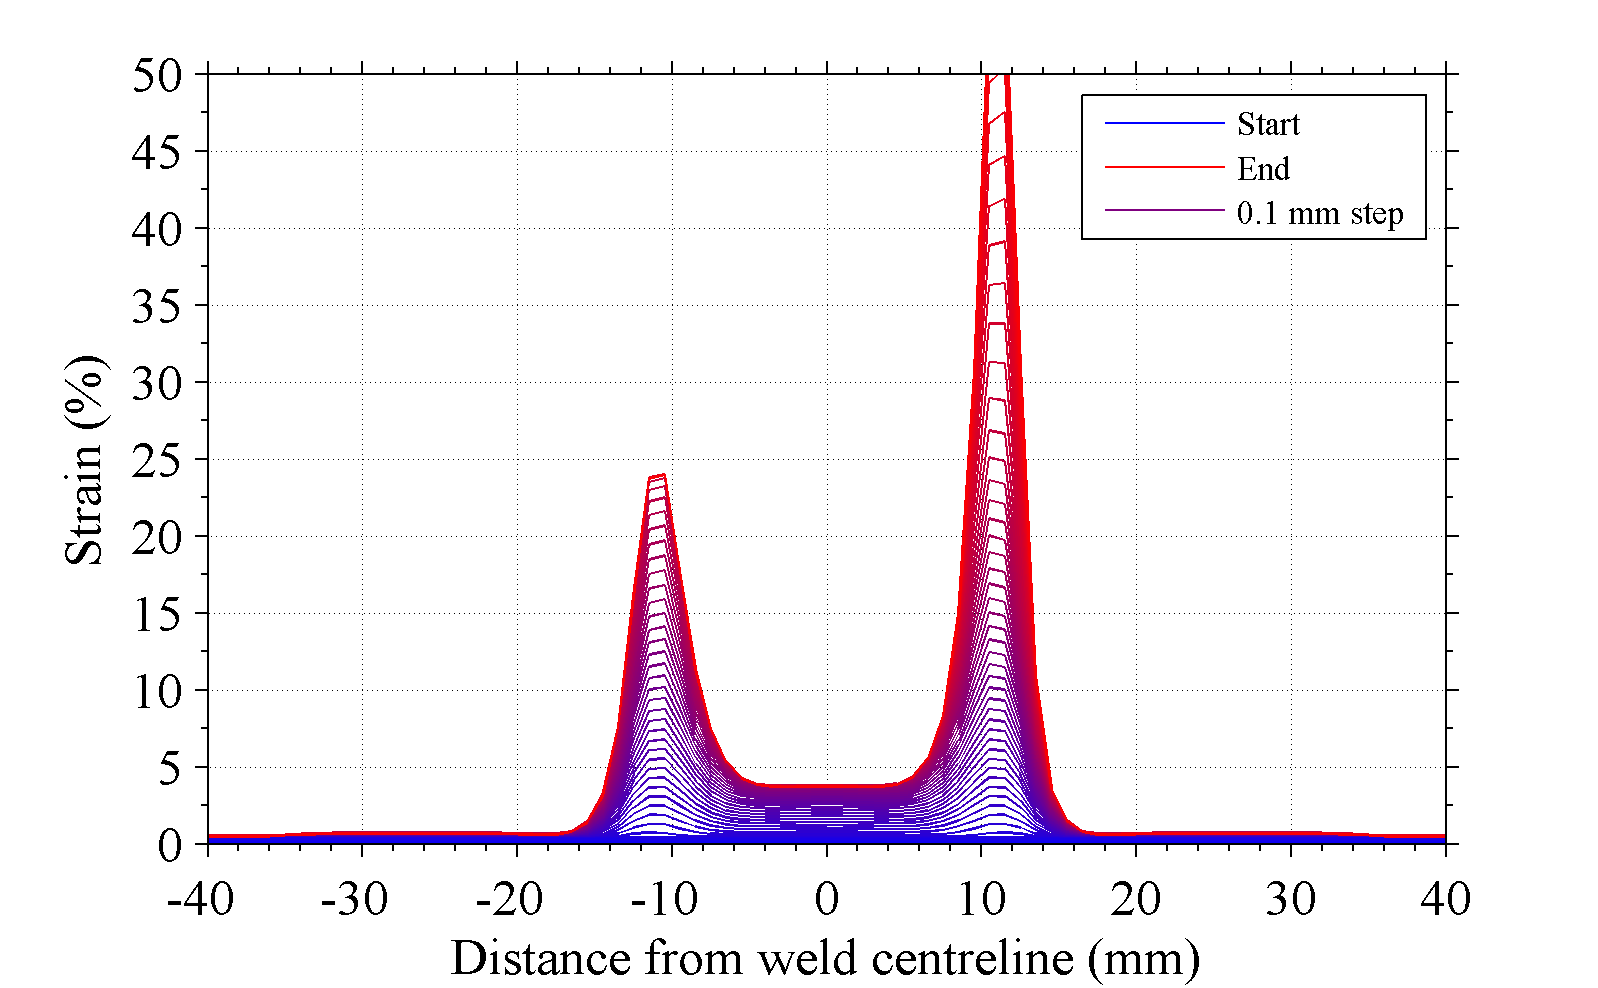
\includegraphics[width=.49\columnwidth]{Figures/ModellingMethod/XStrain_LMCal2altered}}\hfill
	\subfigure[Simulation 4: Hv-step, \textit{k}-constant, \textit{n}-step]{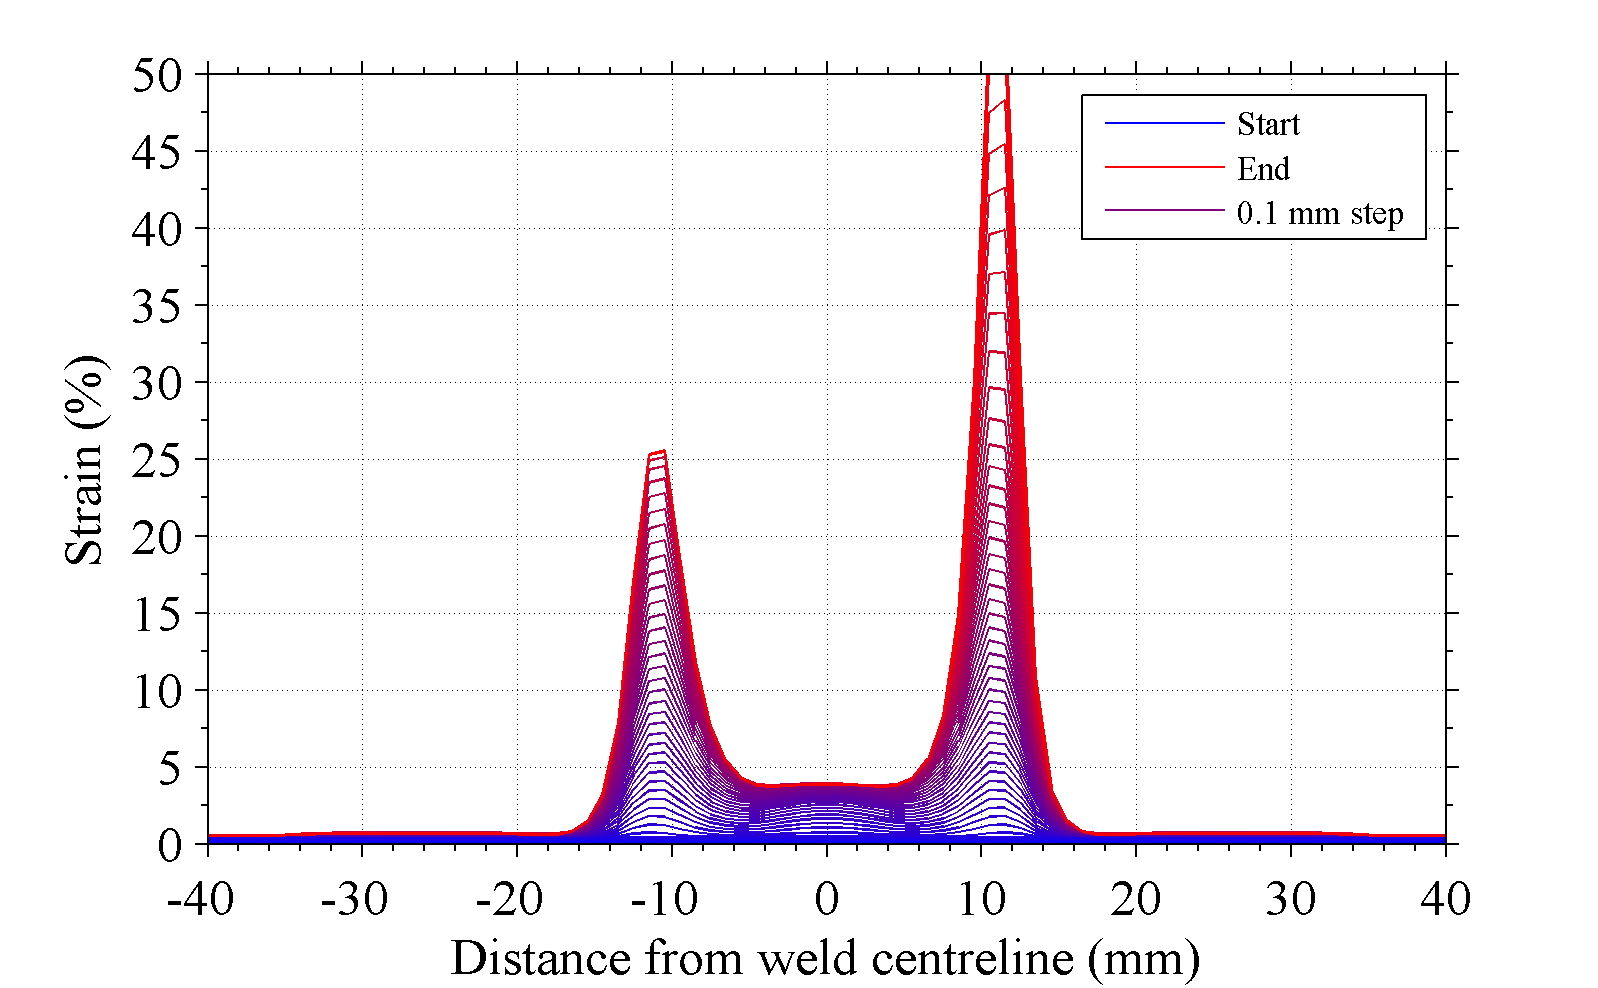
\includegraphics[width=.49\columnwidth]{Figures/ModellingMethod/XStrain_LMCal3altered}}\centering 
	\caption[Strain predictions based on lumped mass method]{Predicted strain distributions based on the lumped mass method. Strain distribution are plotted for every 0.1 mm of global deformation between the ends of the samples. Predicted strain transitions from blue, at the start of the test, to red, at the end of the test. Failure was not incorporated. Note that values of $k$, $B$, and $n$ can be found in figure \ref{fig:Hvdistribution}c-e.}
	\label{fig:LumpedMassPredictions}
\end{figure}

Simulations 1-4 (figure \ref{fig:LumpedMassPredictions}b-e) to show the effects of the lumped mass method, applied both directly and in calibrated forms, on the predicted strain distribution in the weld. In simulation 1 (figure \ref{fig:LumpedMassPredictions}b), the size of the weld zones correlate directly to those observed via optical macrograph. In simulation 2 (figure \ref{fig:LumpedMassPredictions}c), the weld zones are adjusted to capture key features from the hardness distribution of the weld, i.e. the minima in the hardness profile. In simulation 3 (figure \ref{fig:LumpedMassPredictions}d), the weld zones are the same in simulation 2 except that the width of the hardness minima is increased in order to better capture the material properties of the region containing the hardness minima. In simulation 4 (figure \ref{fig:LumpedMassPredictions}e), the weld zones are kept the same as in simulation 3, however, some variation in plastic response is allowed following the method by Genevois et al. \cite{Genevois2006}. This represents the state of the art in terms of current weld modelling techniques adapted from the lumped mass method. 

In comparison to the experimental measurements, we can observe that application of either direct or calibrated forms of the lumped mass method all lead to significantly different behaviour. In simulations 1 and 2 (figure \ref{fig:LumpedMassPredictions}b-c), the methodologies do capture the initial yielding within the nugget region. However, deformation strain remains contained within the nugget region through the length of simulation in either model. The only observable difference is that in simulation 1, deformation strain remains confined to the narrow region of the TMAZ/Nugget, whereas in simulation 2, deformation strain is accomodated over a wider region of the weld. Unlike in the experimental observations, in both simulation 1 and 2, the predicted deformation strain does not transition out of the nugget region. Strain localisation is predicted to be in the centre of the nugget rather than in the position coincident with the hardness minima, as observed in experiment. It must be noted that the predicted response remains symmetric in simulations 1-2, which is consistent with the way the model is initialised. 

In contrast, simulations 3 and 4 (figure \ref{fig:LumpedMassPredictions}d-e) demonstrate a consistent, almost identical, overall response. That response differs, markedly, from simulations 1-2 and the experimental results. The simulations do capture the initial yielding in the nugget region, however, deformation transitions rapidly into the regions either side of the weld centreline associated with the location of the hardness minima. Whilst a transition in the geometric distribution of deformation strain is captured in the simulations, the overall distribution does not correlate with experimental observations. Deformation strain is confined within these two narrow regions either side of the weld centreline throughout the simulation; this is consistent with the double strain localisation effect discussed in chapter \ref{LitRev} \S\ref{LitRev:ModelStructuralQSMacroDistribution}. It must also be noted that despite the models being initialised as symmetrical, the predicted response is asymmetric. In one of the regions associated with the hardness minima, deformation strain is predicted to be greater than on the other side. 


\subsubsection{Simulations based on the method developed in the present chapter}
\label{SMDModellingstudyResultsSims1to4Correction2}

\begin{figure}[!]
	\subfigure[Simulation 5: Hv-smooth, \textit{k}-constant, \textit{B}-constant, \textit{n}-constant]{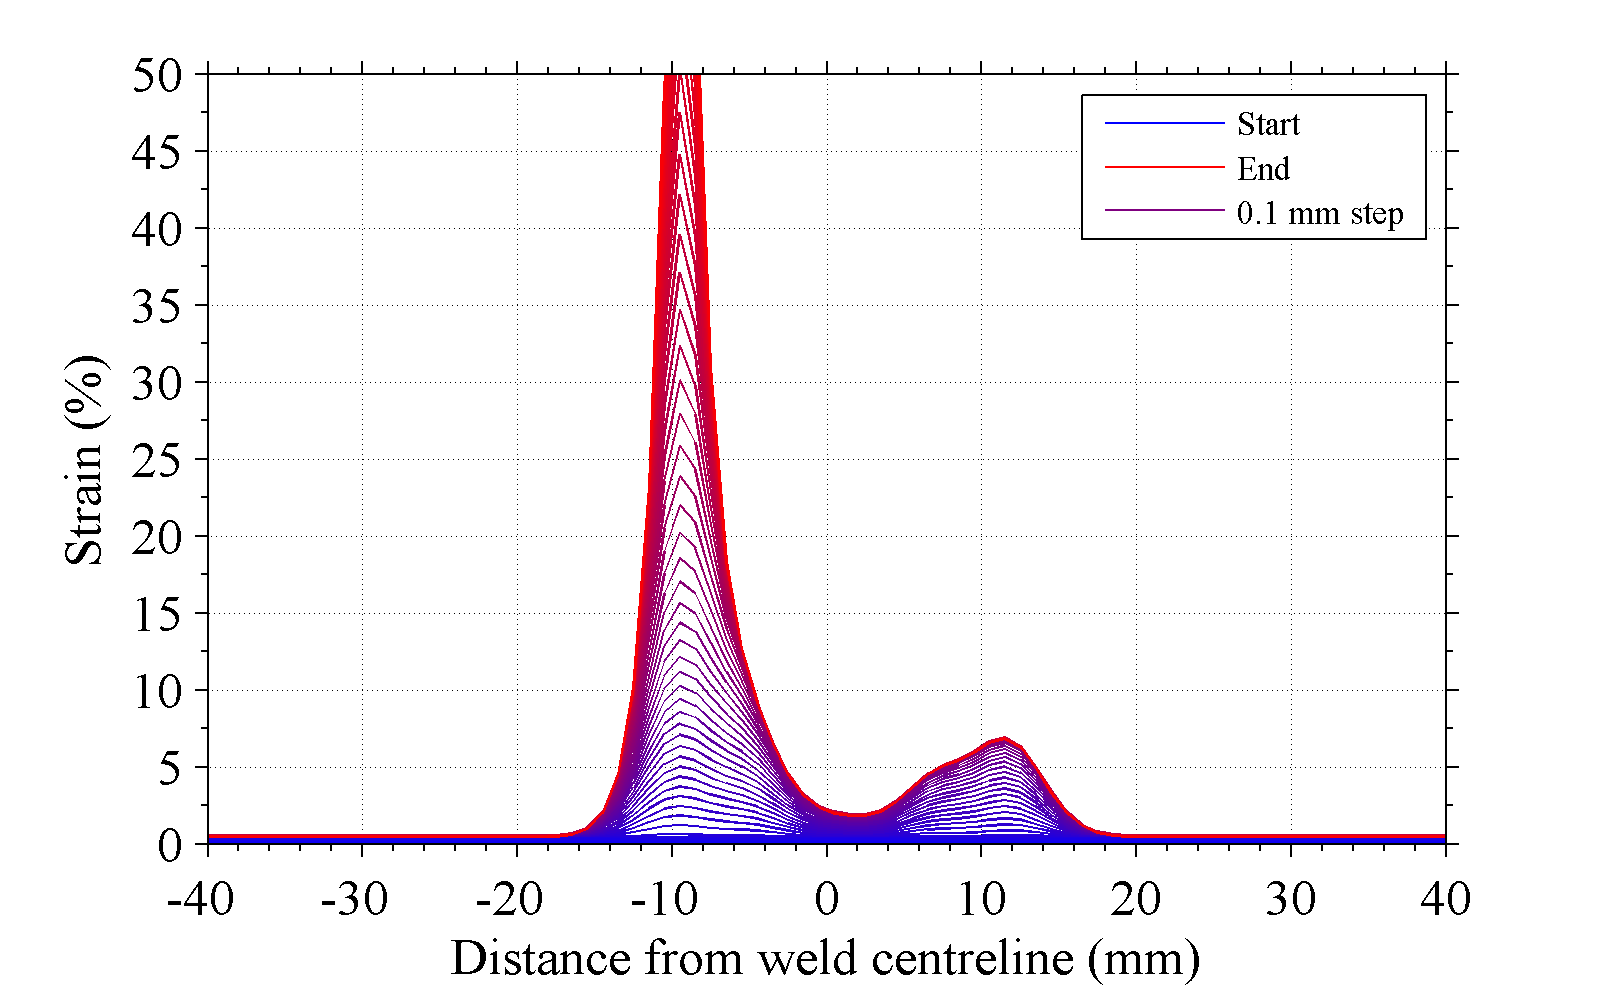
\includegraphics[width=.4\columnwidth]{Figures/ModellingMethod/XStrain_HVSmooth_KConstant_NConstantaltered}}\hfill
	\subfigure[Simulation 6: Hv-smooth, \textit{k}-smooth, \textit{B}-constant, \textit{n}-constant]{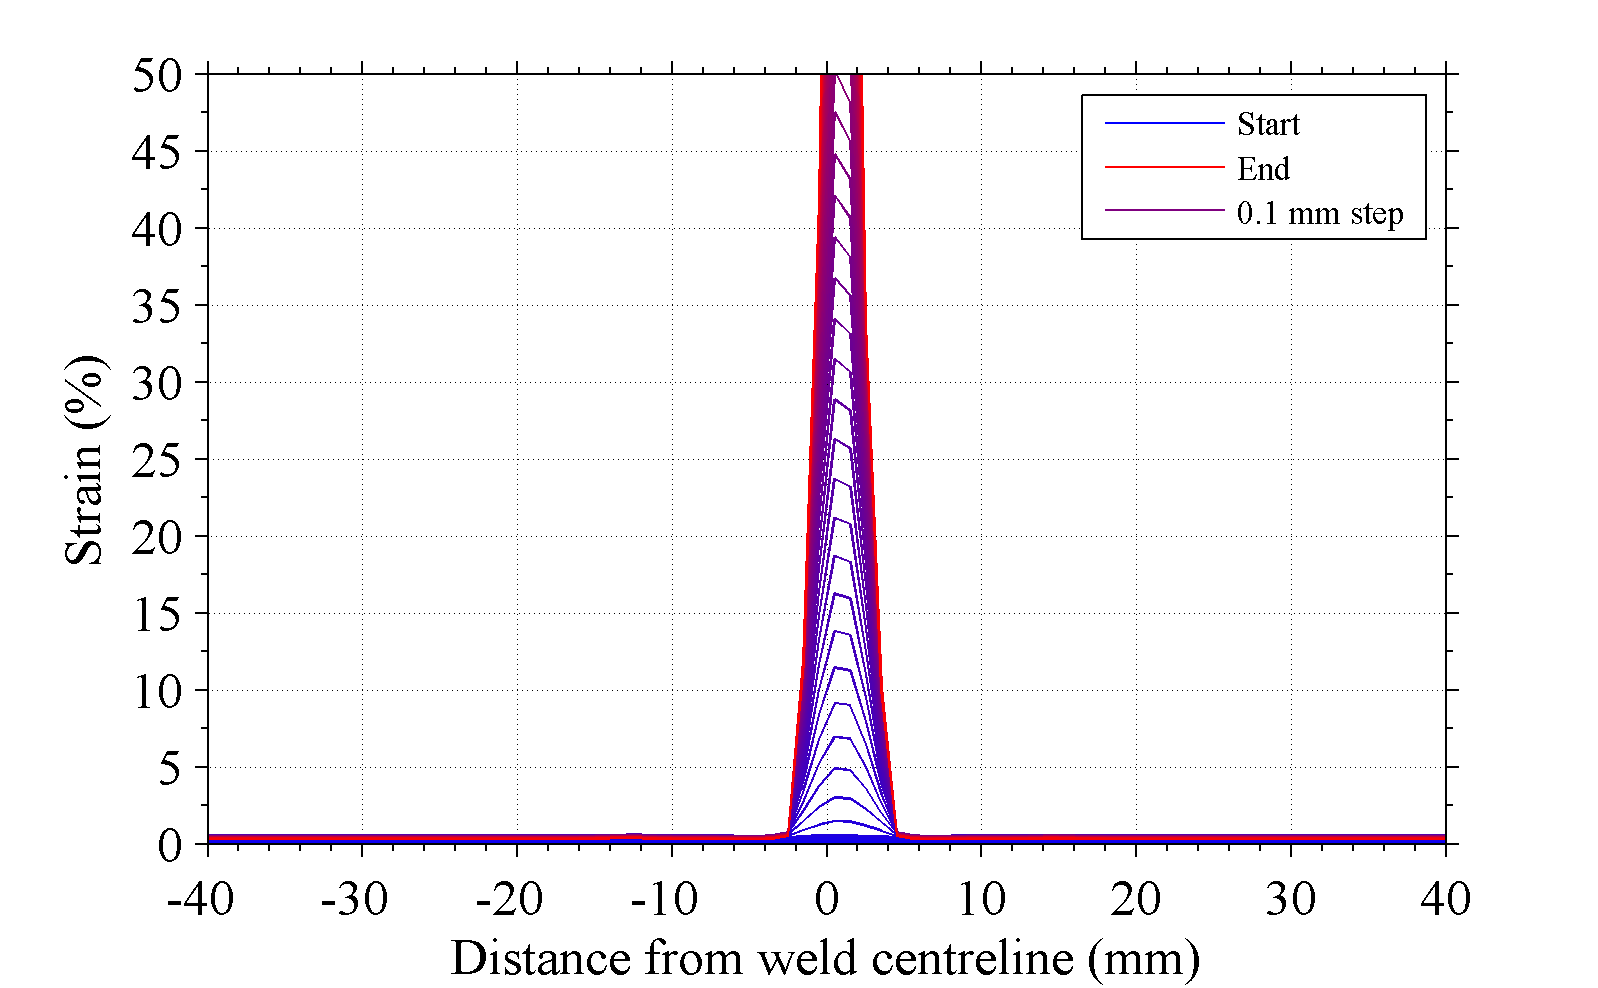
\includegraphics[width=.4\columnwidth]{Figures/ModellingMethod/XStrain_HVSmooth_KSmooth_NConstantaltered}} \hfill
	\subfigure[Simulation 7: Hv-smooth, \textit{k}-step, \textit{B}-constant, \textit{n}-constant]{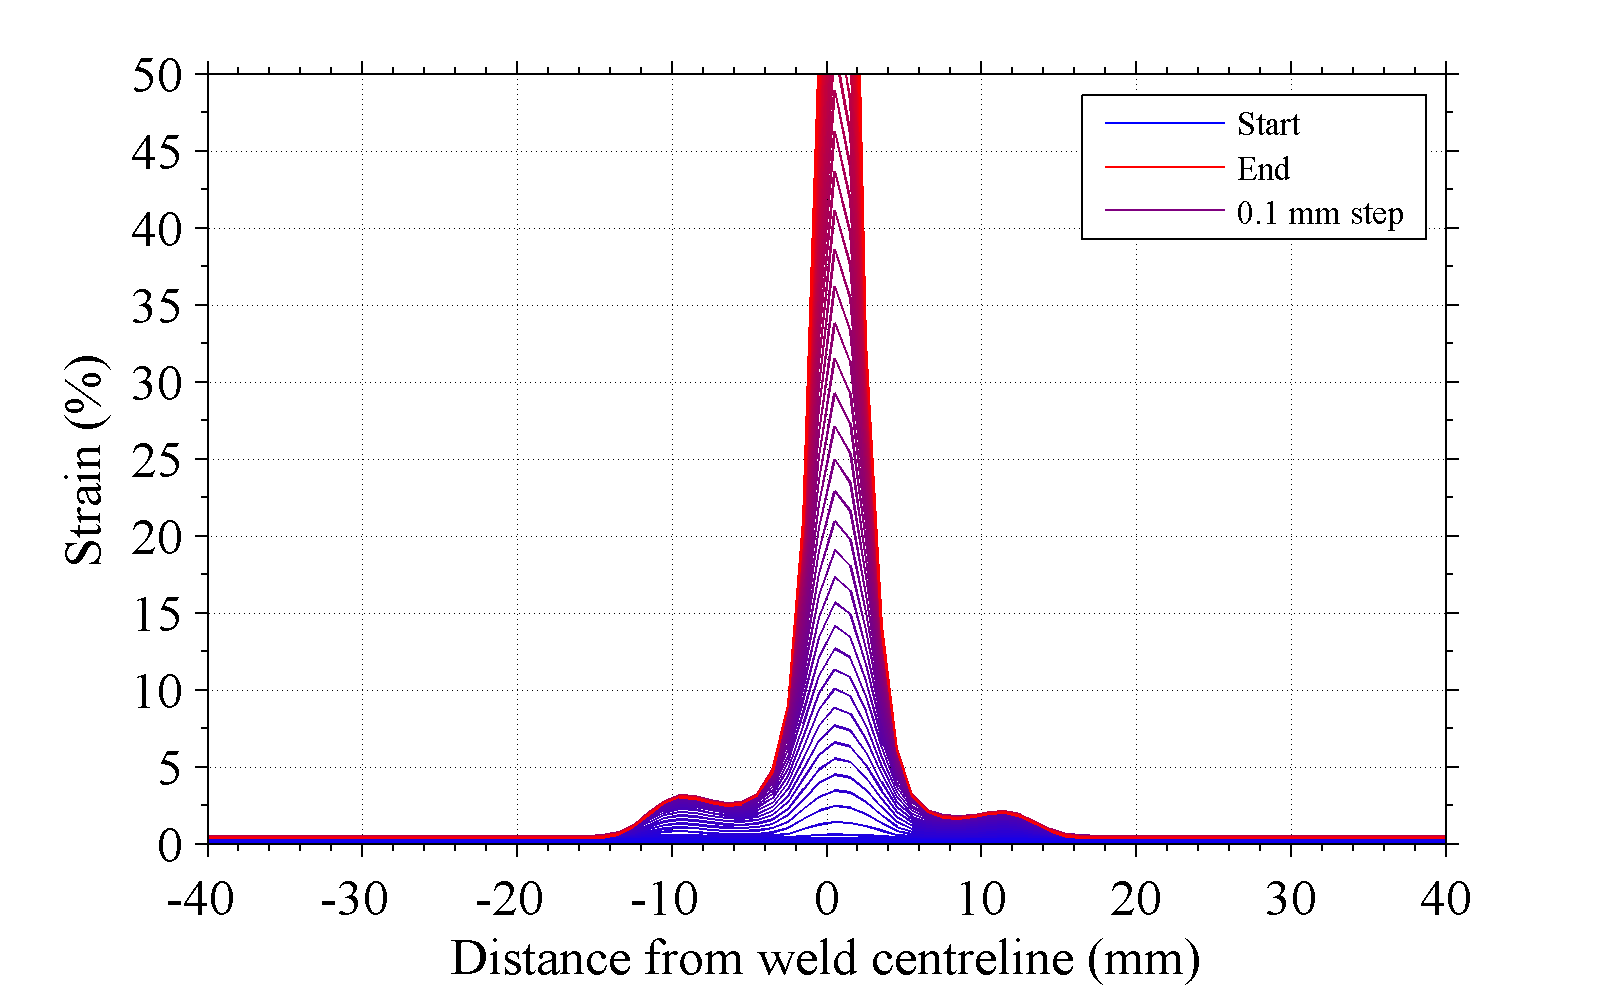
\includegraphics[width=.4\columnwidth]{Figures/ModellingMethod/XStrain_HVSmooth_KStep_NConstantaltered}}\hfill
	\subfigure[Simulation 8: Hv-smooth, \textit{k}-step, \textit{B}-smooth, \textit{n}-smooth]{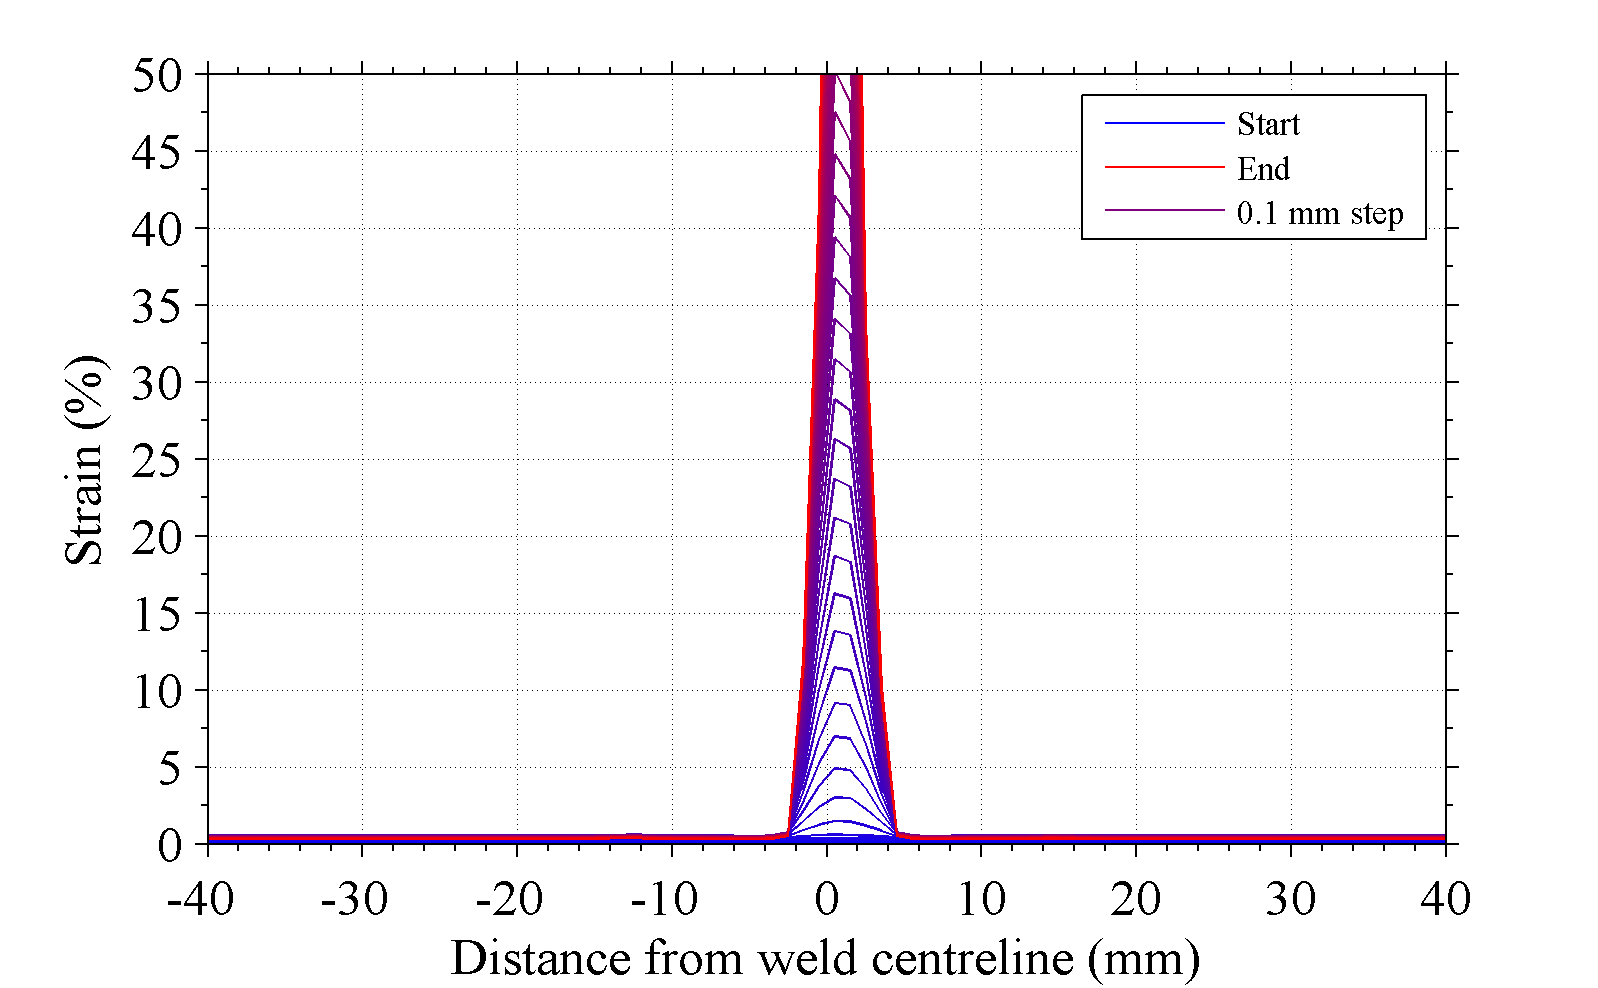
\includegraphics[width=.4\columnwidth]{Figures/ModellingMethod/XStrain_HVSmooth_KStep_NSmoothaltered}}\hfill
	\subfigure[Simulation 9: Hv-smooth, \textit{k}-step, \textit{B}-step, \textit{n}-step]{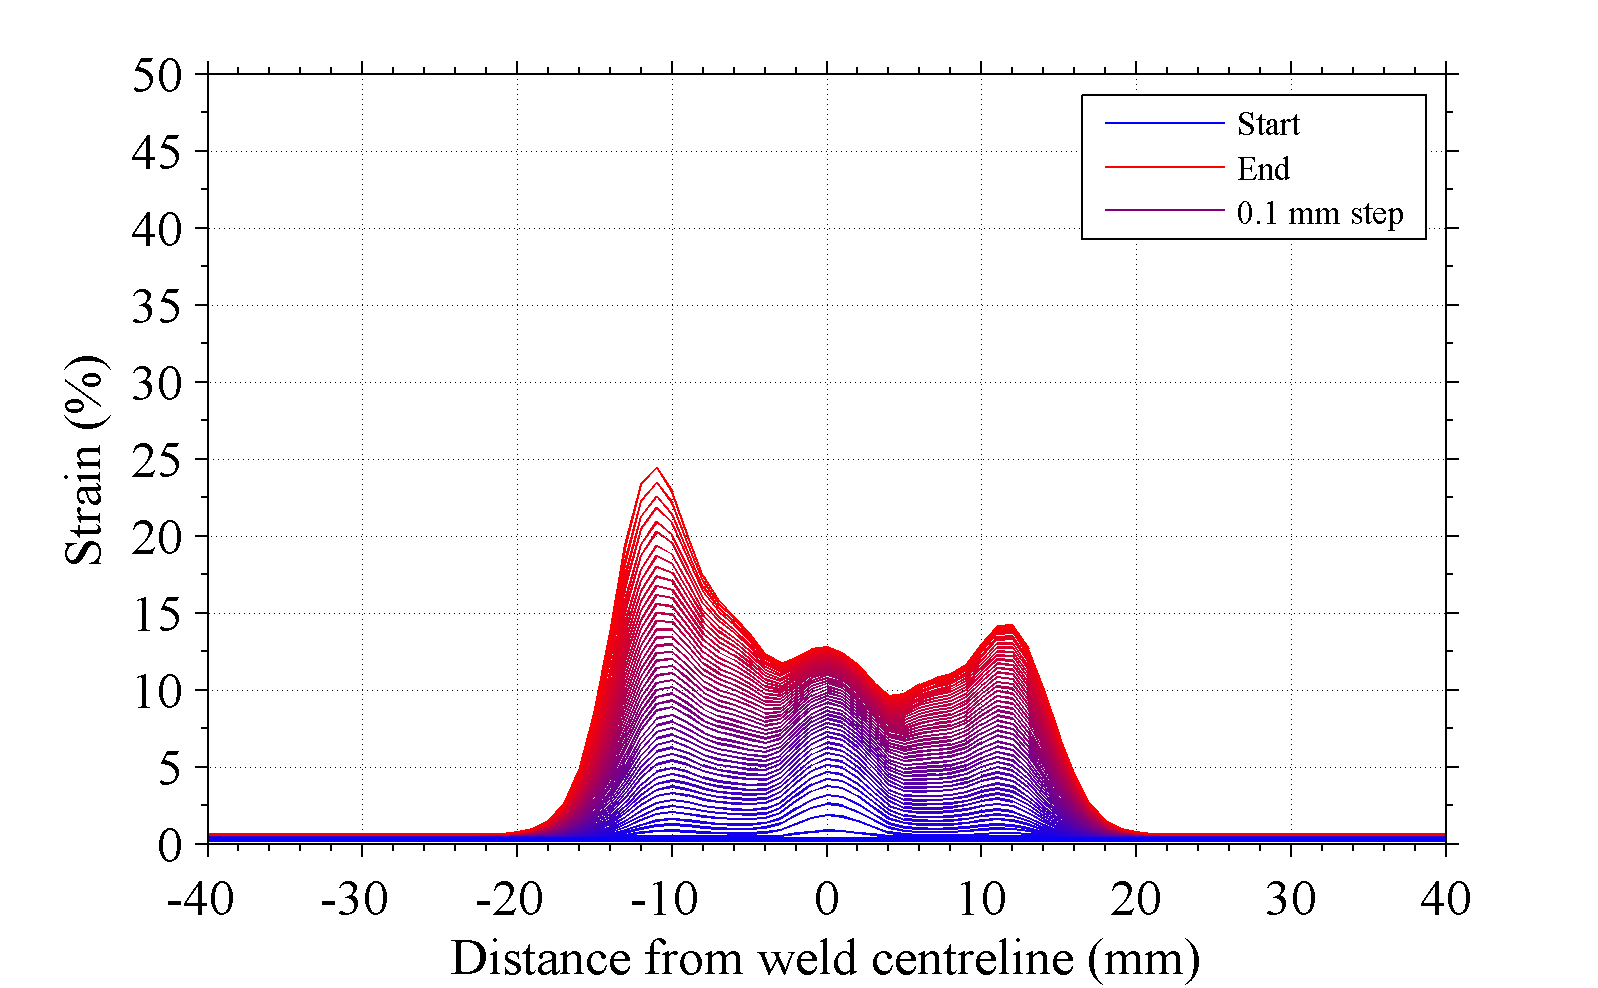
\includegraphics[width=.4\columnwidth]{Figures/ModellingMethod/XStrain_HVSmooth_KStep_NStepaltered}}\hfill
	\subfigure[Simulation 10: Hv-smooth, \textit{k}-step, \textit{B}-step, \textit{n}-step]{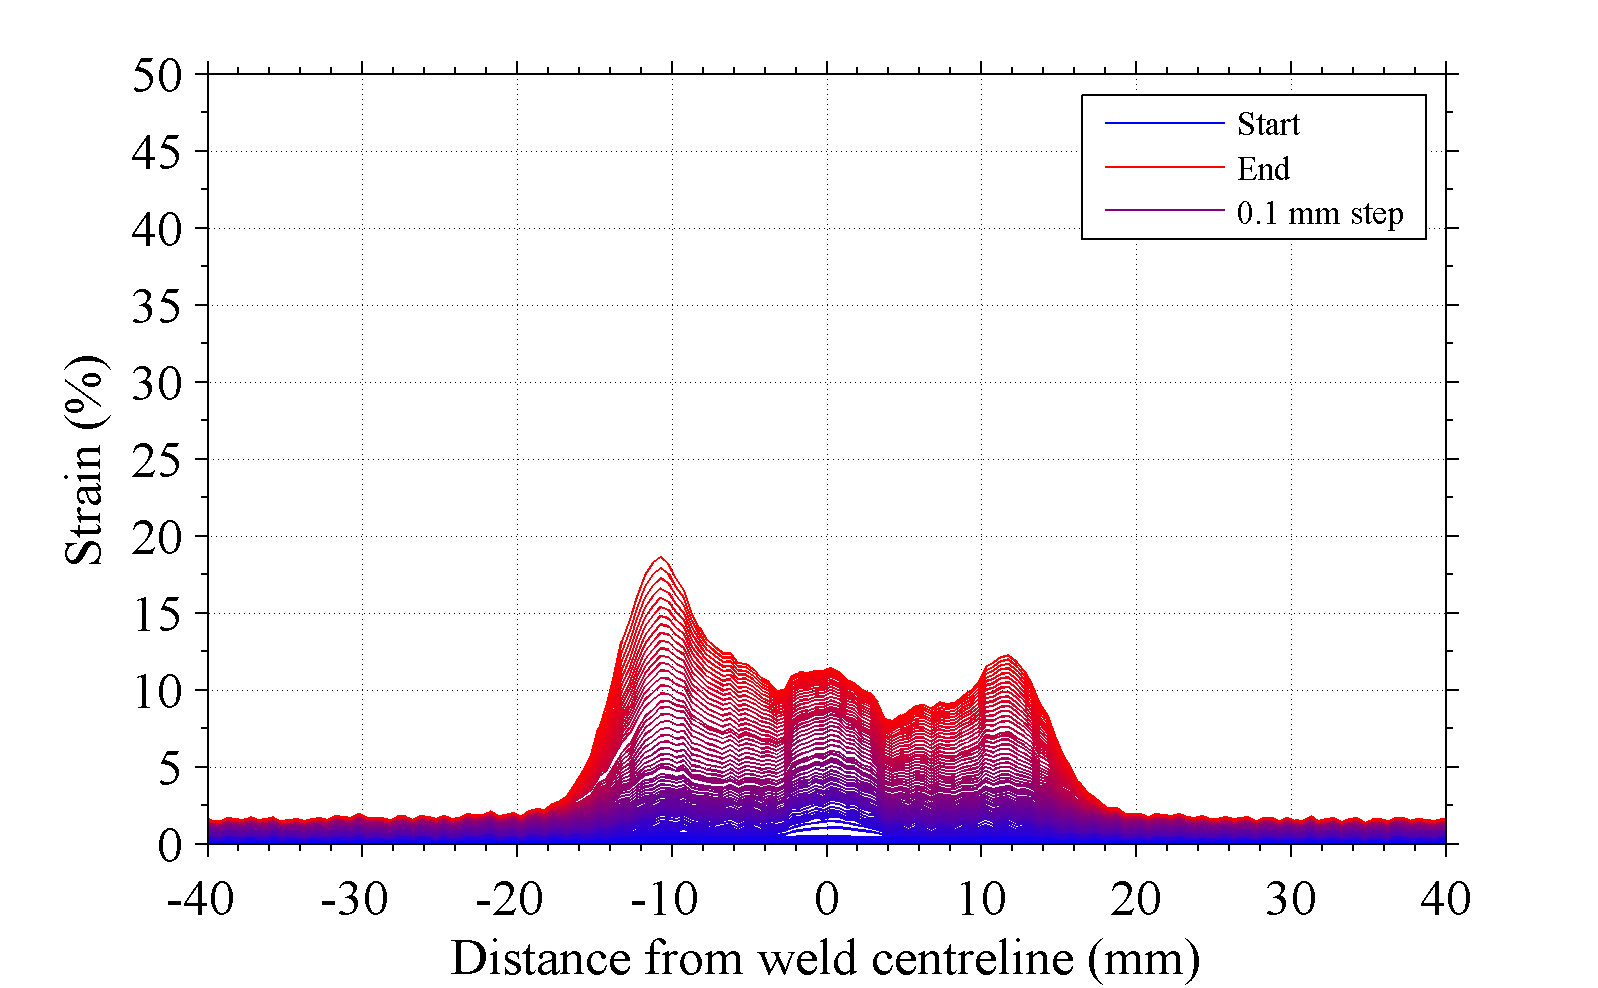
\includegraphics[width=.4\columnwidth]{Figures/ModellingMethod/XStrain_HalfMeshaltered}}\hfill
	\subfigure[DIC measured strain]{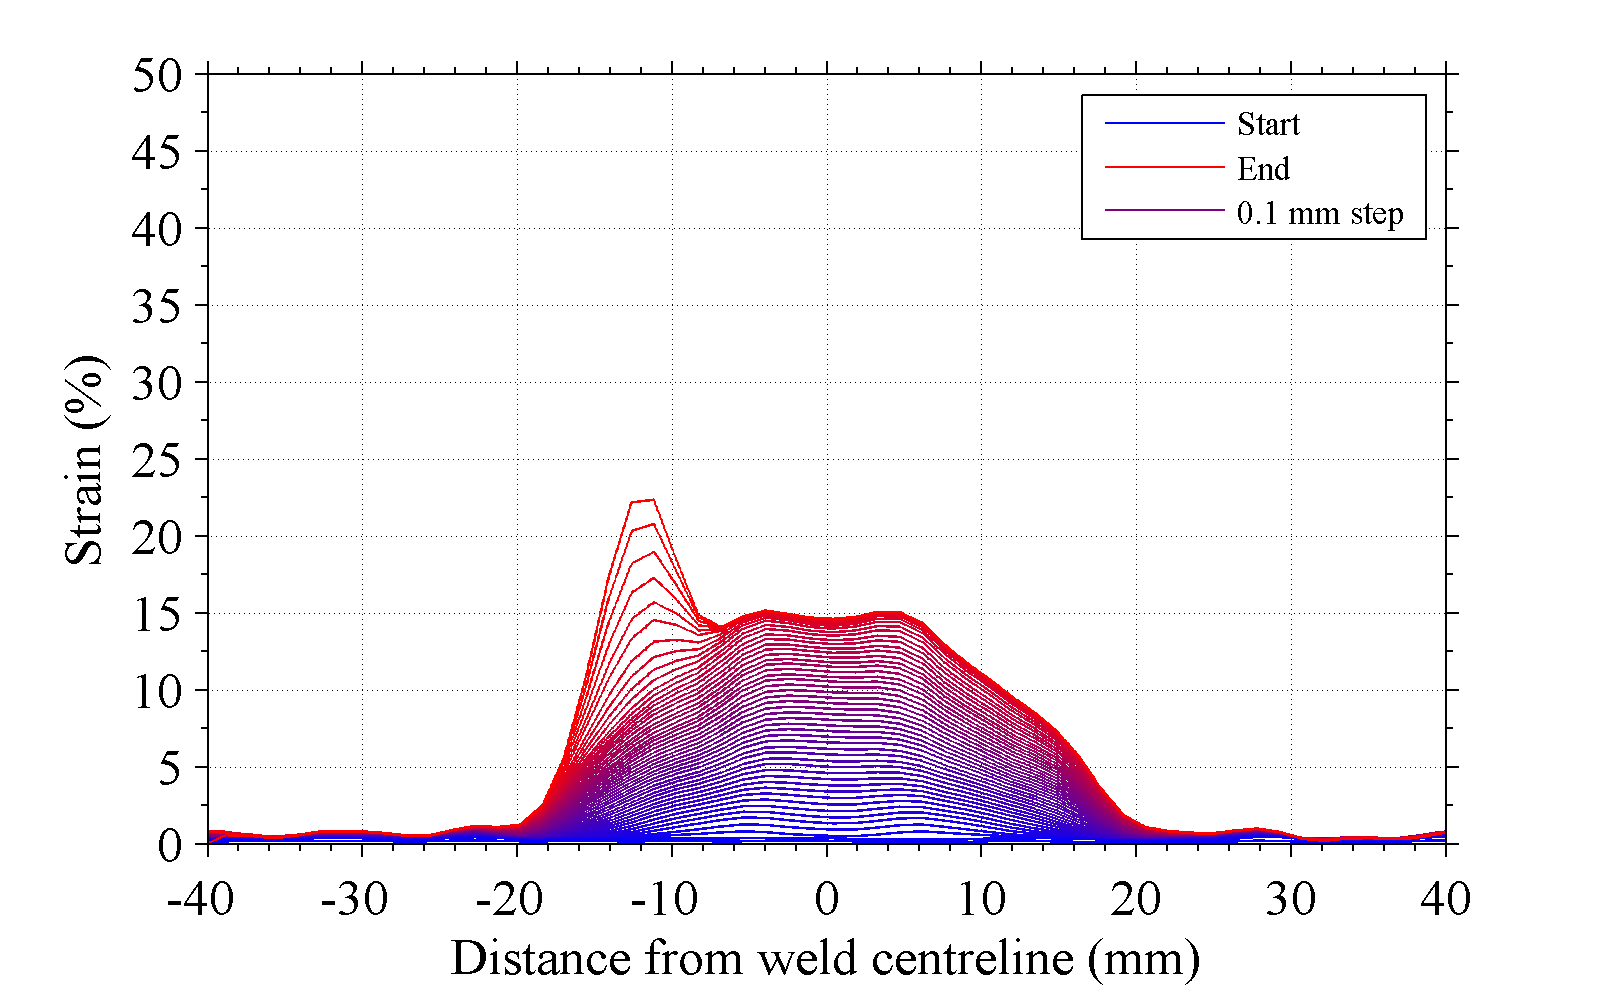
\includegraphics[width=.4\columnwidth]{Figures/ModellingMethod/XStrain_DICMeasuredaltered}}\centering
	\caption[Strain predictions based on systematic incorporation of complex mechanical properties]{Predicted strain distributions by systematically varying the yield stress and plastic behaviour. Strain distribution are plotted for every 0.1 mm of global deformation between the ends of the samples. Predicted strain transitions from blue, at the start of the test, to red, at the end of the test. Failure was not incorporated. Note that values of $k$, $B$, and $n$ can be found in figure \ref{fig:Hvdistribution}c-e.}
	\label{fig:Systematicmechs}
\end{figure}

Simulations 5-10 systematically demonstrate the effects of modelling method developed in the present chapter. Simulation 5-7 show the effects of the yield stress distribution, as influenced by the variation in relationship between hardness and yield stress ($k$-parameter). Simulations 7-9 show the effects of the plastic response, as defined by the upper and lower bound distributions of the $B$ and $n$-parameters. Simulation 10 is a numerical mesh convergence study demonstrating the stability of the numerical simulation method using the optimal property distributions, which are identified as those in simulation 9. 

%Simulation 5 has the same user input parameters as the lumped mass method (simulation 3), except for the diffuse distribution of hardness. In addition, simulations 5-7 all have equivalent user input hardness and plasticity parameters, and the only difference arises from the user input $k$-parameter distributions. 
Simulation 5 (figure \ref{fig:Systematicmechs}a) shows an initial yield yield response similar to the lumped mass method found in simulation 3 (figure \ref{fig:LumpedMassPredictions}d). Initial yielding occurs in the regions associated with the hardness minima, however, deformation strain is accommodated over a much wider region of the weld compared to the lumped mass method. Simulation 5 shows that strain distribution increases across the weld region with increasing global deformation, similar to simulation 3. However, in contrast to simulation 3, strain begins to localise on the side of the weld associated with the lowest hardness minima; simulation 5 does not exhibit a double strain localisation effect. Simulation 7 (figure \ref{fig:Systematicmechs}c) shows a similar initial response to simulation 5, however, the overall increase in strain across the weld is lower. Moreover, final strain localisation occurs in the nugget instead of at the hardness minima. 

In contrast, both simulation 6 (figure \ref{fig:Systematicmechs}b) and simulation 8 (figure \ref{fig:Systematicmechs}d) show initial yielding in the nugget region followed by strain localisation; deformation strain remains contained within the nugget throughout the length of the simulation. The predicted response in both these simulations is markedly different from the experimental results figure \ref{fig:Systematicmechs}g). 

Simulations 9 (figure \ref{fig:Systematicmechs}e) and 10 (figure \ref{fig:Systematicmechs}f) show a consistent response, which correlates reasonably with the experimentally measured result (figure \ref{fig:Systematicmechs}g). Initial yielding occurs over the nugget region of the weld, and, under increasing global deformation, strain evolves over an increasing proportion of the HAZ. Eventually, plastic strain begins to localise at the location coincident with the hardness minima. The main difference between simulation 9 and 10 is that the absolute values of the plastic strain distribution across the weld are slightly lower with the refined mesh.
%TODO finish results description of simulations 5-10 (SHERCLIFF CORRECTION)

For simulation 9, the global strain distribution is presented in figure \ref{fig:MacroStrains}b; the associated global stress-strain curve with positions $t_1 - t_5$ is shown in figure \ref{fig:GlobalStressStrain}. It is clear that the overall distribution correlates reasonably well with the experimentally measured strain in the weld cross section, as shown in figure \ref{fig:MacroStrains}a. It should be noted that a diffuse distribution of plastic strain is observed in the HAZ. 

% % % % % % % % % % % % % % % % % % % % % % % % % % % % % % % % % % % % % % % % % % % % % % % % % %
% % % % Discussion
% % % % % % % % % % % % % % % % % % % % % % % % % % % % % % % % % % % % % % % % % % % % % % % % % %
\section{Discussion}
\label{Discussion}
In this discussion, focus shall be given to interpreting the predicted deformation response of the weld under loading in comparison to the experimentally measured response. This enables the effect of the user input mechanical property distribution to be understood more readily. The discussion highlights some of the practical difficulties and limitations in both applying the lumped mass method and interpreting numerical predictions based on the associated assumptions. Furthermore, the discussion identifies some key requirements, in terms of defining complex mechanical property distributions, which are necessary for accurate and reliable predictions of the local strain distribution. Moreover, the discussion provides insight to the true distribution of mechanical properties within an actual weld, and its relationship with microstructure.

\subsection{Interpretation of experimental results}
\label{SMDModellingstudyDiscussionReality}
From the experimentally measured axial strain distributions, on both a macro and more local scale, it is clear that initial yielding occurs across both the TMAZ and nugget. The measured local axial strain distribution suggests that axial strain maybe slightly higher within the TMAZ, though the distribution is relatively uniform over these two regions. Nevertheless, the observed initial yielding response is consistent with directly comparable experimental data presented by McWilliams et al. \cite{McWilliams2013} Moreover, this observed initial response should be expected; the measured mechanical properties from representative weld material, as presented in \S\ref{RADMechPropsResultsQS} chapter \ref{ResultsMicrostructure}, suggest that initial yield stress is lowest within the TMAZ/nugget region. It is useful to note at this point that despite the minimum hardness in the weld being within the HAZ, initial yielding occurs in the TMAZ/nugget region. This indicates that the \textit{k}-parameter distribution decreases towards the centre of the weld, which is consistent with observations of the mechanical properties as estimated from the representative weld material presented in chapter \ref{ResultsMicrostructure}. This complex distribution of the $k$-parameter must, therefore, be an important consideration for accurate modelling of the non-linear weld response.  

As global deformation continues, the flow stress increases in the bulk region incorporating both the nugget and TMAZ via work hardening. This enables the immediately surrounding region of the inner HAZ to yield and begin to accommodate deformation strain. This process continues with global deformation, enabling a progressively wider region of the weld to yield and accommodate deformation strain. Within the outer HAZ, the peak axial strain measured decreases gradually, or diffusely, with increasing distance from the weld centre. This response should be expected because local flow stress is dominated by the volume fraction of $\Omega$ phase, which decreases gradually towards the centre of the weld. The volume fraction is linked to the gradual dissolution of $\Omega$ phase in the weld \cite{McWilliams2013,Grujicic2011}; this process is a function of the peak temperature experienced during the weld thermal cycle \cite{Sullivan2011,Robson2006}. 

At the critical point, axial strain begins to localise at the position coincident with the location of minimum hardness in the weld, which can be interpreted to occur due to two reasons. Firstly, the bulk inner region of the weld (i.e. the region confined between both hardness minima) has a larger capacity for work hardening than the outer regions, as estimated from the representative weld material. This is important because it causes the flow stress of the inner region to increase at a faster rate than the outer regions, owing to the difference local work hardening response. The estimated stress-strain response predicted by the constitutive models of the representative weld material (table \ref{tab:JCParameters}) suggests that when the inner HAZ and TMAZ/nugget regions are deformed beyond approximately 10\% plastic strain, the flow stress in the TMAZ/nugget and inner HAZ will be consistently greater than the flow stress in the outer HAZ; this is due to the difference in the work hardening response. More succinctly, the stress-strain curves of the inner HAZ and nugget/TMAZ cross over the stress-strain curve of the outer HAZ, as shown in figure \ref{fig:ConstitutiveModels}.

Secondly, since there is a decreasing distribution in flow stress in the outer HAZ towards the centre of the weld, linked to the decreasing volume fraction of $\Omega$ phase, axial strain will be distributed such that it is increasing towards the weld centreline. However, the strain distribution but will be constrained by the mismatch in flow stress at the interface between the inner and outer HAZ (where the stress-strain curves cross over each other). Hence, the onset of strain localisation and necking occurs at the interface of the inner and outer HAZ. For 2139-T8, this position is coincident with the location of minimum hardness in the weld. As the mechanical properties of 2139-T8 are dominated by $\Omega$, the hardness distribution represents a good indicator of final strain localisation, due to the characteristic mechanical property distribution within the weld cross section that are linked to the microstructure. However, the hardness minima cannot be assumed to define the probable failure location for a general precipitate hardened aluminium alloy. This is because the hardness distribution is not always unambiguously indicative of the local mechanical property distributions in the weld, particularly the plastic response of the weld regions. As mentioned in the literature review, under aged alloys, or alloys strengthened by a more than one dominant strengthening phase have a more complex relationship with hardness.

\begin{figure}[h!]
	\centering
	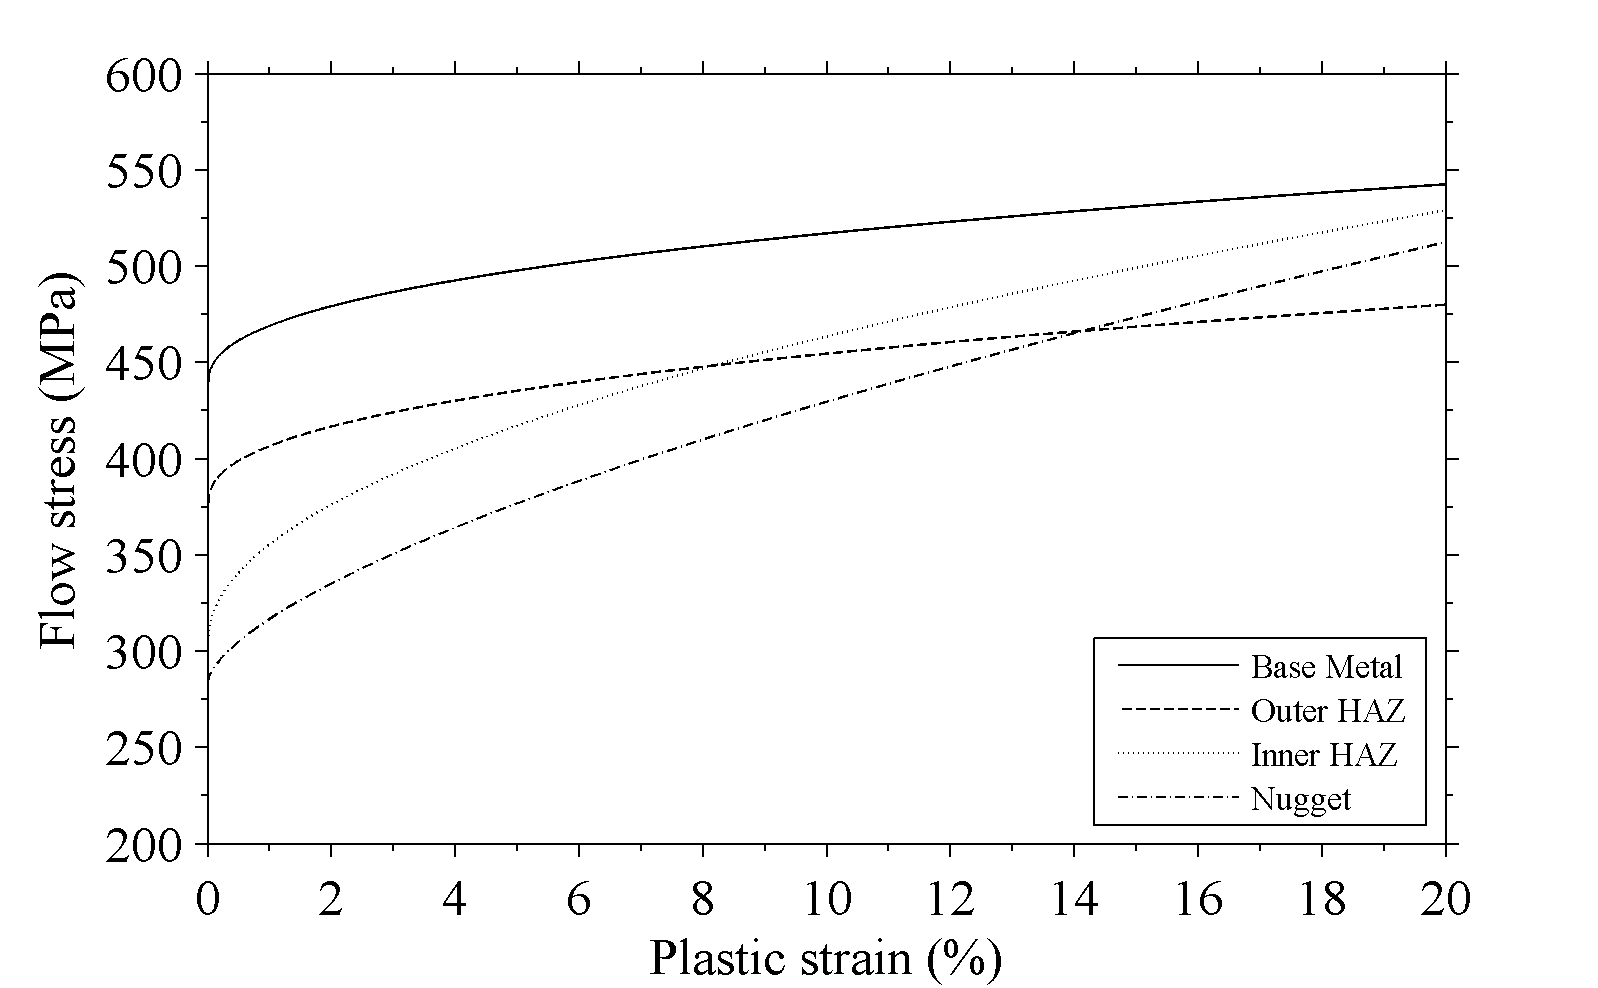
\includegraphics[width=.8\linewidth]{Figures/ModellingMethod/ConstitutiveModelsaltered}
	\caption[Local stress strain response of weld regions]{The plastic stress-strain response of the different local regions of the weld according to the Johnson-Cook parameters in table \ref{tab:JCParameters}. Note that the stress-strain curves of the inner regions of the HAZ and the TMAZ/Nugget cross over the stress-strain curve of the outer HAZ after a critical plastic strain; this is due to the difference in work hardening response.}
	\label{fig:ConstitutiveModels}
\end{figure}

The interpretation of measured strain distributions can be assumed to be reasonably accurate on a local scale, because DIC measurements following the method outlined in chapter \ref{ExperimentalMethods} are estimated to provide strain measurements to an accuracy of $\pm 0.05$\% strain \cite{DaFonseca2005}. The reliability of the method can be assessed by comparing the strain measurements to strain gauges or extensometers. Whilst, it is not presented here for brevity, the global engineering strain response was comparable to the response measured using an extensometer; the global engineering strains are $\pm 0.1$\%, for engineering strains of $\leq 15$\%, and $\pm 1$\%, for engineering strains of $\leq 20$\%. There is a divergence in correlation with extensometer readings at larger strains, however, the extensometer does not account for necking. It is more likely that the strain measurements are more representative of the actual response using DIC despite this apparent reduction in reliability, though this does depend on the coherency of the paint with the sample surface. Nevertheless, the interpretation of the experimentally measured response can be assumed to be fairly reliable. Moreover, the interpretation correlates with the estimated local mechanical properties and can be linked to the observed microstructural variation.

\subsection{Interpretation of simulations based on the lumped mass method}
\label{SMDModellingstudyDiscussionLumpedMassMethod}
As will be discussed here, practical application of the lumped mass method to FSW, whether direct or in a calibrated form, as described in the literature, is not straightforward and can lead to complications from both a metallurgical perspective and a numerical modelling perspective. There is a trade-off between the metallurgical similarity of the model with the actual weld and both the numerical accuracy and reliability of the predicted results. Using direct application of the lumped mass method, metallurgical similarity is promoted, whereas through a calibrated approach, numerical accuracy is promoted. In this section, the commonly used methods are discussed based on the results described in \S\ref{SMDModellingstudyResults}. 

As mentioned in \S\ref{LitRev:ModelStructuralQSMacroDistribution} chapter \ref{LitRev}, under the lumped mass method, the weld region is partitioned into distinct regions, which are representative of the nugget, TMAZ, HAZ, and parent material. Partitioning is based on the hardness distribution and observation of macrographs of the weld cross section. The distinct nugget and TMAZ region are easily determined, geometrically, from the weld macrographs, and the unaffected zone can be identified from the hardness distribution. Homogenising the elements of the mesh into the four basic regions does make logical sense from a simplified metallurgical perspective, though it is dependent on welding conditions. However, as will be discussed, from a numerical modelling perspective, this is not always appropriate, as there are unintended consequences if the assumptions of the lumped mass method are applied exactly. As a result, calibrated forms of the lumped mass method are used to accommodate the effects of these assumptions. However, there are always limitations to the results, and care must be taken during interpretation of their validity, as shall be discussed here. As a reminder, the basic assumptions of the lumped mass approach are that: yield stress scales directly with hardness; the linear coefficient relating hardness to yield stress is constant across the weld; there is no variation in work hardening behaviour across the weld.

%Hugh Shercliff correction
%\paragraph{Calibration}
\subsubsection{Calibration}
\label{SMDModellingstudyResultsSims1to4Correction1Calibration}
Simulation 1 represents direct application of the standard lumped mass method, as described in chapter \ref{LitRev}. In this case, the widths of the bulk weld region, as defined by the hardness distribution, are representative of the weld cross section from a metallurgical perspective. However, as shown in figure \ref{fig:Hvdistribution}a, the minima of the hardness distribution across the weld is neglected even though it is the point associated with strain localisation. In addition, the plastic response across the weld is assumed to be equivalent to the parent material. From a numerical perspective, key regions of the weld are neglected from the model which are sources of error.

Simulation 2 represents a calibration of the standard form of the lumped mass method; the width of the nugget region has been artificially increased and also incorporates the TMAZ and inner HAZ regions. The modelled TMAZ has become a narrow region associated with the minima of the hardness distribution of the weld, as shown in figure \ref{fig:Hvdistribution}a. In addition, the plastic response across the weld is assumed to be equivalent to the parent material. From a metallurgical perspective, this method is less representative of the weld cross section compared to simulation 1. However, the region incorporating the hardness minima is captured in the model, which is an improvement from a numerical perspective. 

Simulation 3 represents further calibration to the lumped mass method in simulation 2; the width of the nugget region remains artificially increased to incorporate the TMAZ and inner HAZ. The width of the TMAZ region has also been increased (artificially) but remains associated with the minima of the hardness distribution of the weld, as shown in figure \ref{fig:Hvdistribution}b. The plastic response across the weld is still assumed to be equivalent to the parent material. From a metallurgical perspective, this method is less representative of the weld cross section compared to simulation 2. However, the relative importance of the region incorporating the hardness minima has incresed, which would serve to improve numerical accuracy of the simulation.

Simulation 4 represents further calibration to the lumped mass method in simulation 3, and is equivalent to the method used by Genevois et al. \cite{Genevois2006} to model the structural response of aluminium welds. The width of the nugget region remains artificially increased to incorporate the TMAZ and inner HAZ, and the width of the TMAZ region remains artificially increased and associated with the minima of the hardness distribution of the weld, as shown in figure \ref{fig:Hvdistribution}b. However, the plastic response across the weld is no longer assumed to be equivalent to the parent material and local plastic response is specified. From a metallurgical perspective, this method is as representative of the weld cross section as simulation 3. From a numerical perspective, there is additional information about the work hardening response which serves to improve the accuracy of the simulation.

It can interpreted that calibration of the lumped mass method is performed in order to achieve good correlation between the predicted and experimentally measured global stress-strain response of the weld. Nevertheless, exact details of calibration methods are typically omitted from studies in the literature. Calibration allows important features of the weld, such as the hardness minima, to be captured using the lumped mass method. Hence, calibration is a trade-off between metallurgical similarity of the numerical model with physical reality, and known key features of the weld. However, from figure \ref{fig:LumpedMassPredictions}a-e, it is clear that application of the lumped mass method, either directly or in a state-of-the-art calibrated form, is unsuitable for 2139-T8 alloy. There are significant differences between the predicted and experimentally measured strain evolution under loading. These differences manifest primarily in the initial yield response and the geometrical evolution of strain due to work hardening; these are discussed further in the following paragraphs.

\subsubsection{Initial yield response}
\label{SMDModellingstudyResultsSims1to4Correction1Initialyielding}
The user input hardness profile is directly indicative of initial yield response, since hardness and yield stress are assumed to have a linear relationship that is constant across the weld. Therefore, in simulations 1-4, the lowest theoretical yield stress is effectively in the TMAZ, followed sequentially by the nugget, HAZ, and parent material. It is expected, therefore, that the TMAZ yields first, and as it work hardens, the increase in flow stress will allow the elements associated with the nugget to yield and accommodate deformation strain. As the flow stress in the TMAZ and nugget increases via work hardening, the elements in the HAZ will begin to yield. 
%Since there is no variation in the input work hardening response, the distribution of axial strain is not expected to evolve, geometrically, over time; axial strain should eventually localise in the TMAZ after necking. In addition, since the user input properties are symmetric, a symmetric strain response is expected.  

In contrast to the expected initial yield response, figure \ref{fig:LumpedMassPredictions}b-c (simulations 1-2) both show that initial yielding actually occurs in the elements associated with the nugget and that the majority of axial strain is accommodated within the nugget region throughout the entire simulation. 
%As global deformation continues, axial strain continues to increase within the TMAZ and nugget, and is greatest in the centre of the weld. The predicted strain distribution is symmetric about the weld centreline throughout the simulation. 
The result suggests that the elements within the TMAZ are behaving as if they had a greater flow stress compared to the nugget region. As described in chapter \ref{LitRev}, the lumped mass method causes an artificial increase in the elemental stiffness at the partition of the weld zones. This effect is exacerbated by the low number of elements in the TMAZ across the weld (1) and is most pronounced in both simulation 1 and simulation 2. It also shows that in these important regions, which may be relatively narrow, an appropriately larger number of elements should be used to model the region in order to avoid errors in the numerical solution. 

Therefore, the source of the numerical error can be traced back to the calibration stage, and is exacerbated by the assumptions in simulation 1 and 2. In simulation 1, the TMAZ is approximately 800 $\mu$m wide thus is represented by a single 1x1x1 mm element. In simulation 2, the TMAZ represents the region encompassing the hardness minima. Since the hardness measurements are taken at 1 mm intervals, the TMAZ is also represented by a single 1x1x1 mm. Hence, all the elements of the TMAZ share common nodes with the surrounding elements of the nugget and HAZ; these regions have a greater yield stress than the TMAZ itself. Thus, the elements associated with the TMAZ are constrained to deform with the surrounding elements, thereby demonstrating an artificial increase in elemental stiffness. Since the absolute difference between the assigned yield stress of the nugget and TMAZ is relatively small, the elements of the TMAZ do not yield first despite being assigned the lowest initial yield stress. These elements are shielded due to their increased stiffness, and deformation is confined to elements with the second lowest yield stress, i.e. the nugget. %Moreover, since the work hardening response does not vary, local flow stress in the nugget and TMAZ will never exceed the flow stress of the surrounding elements. Hence, strain is accommodated by the elements of the TMAZ and nugget throughout the simulation, which correlates with theoretical expectations. 

In simulations 3-4, the problem of artificially increasing elemental stiffness is attenuated by increasing the effective width of the TMAZ during calibration. This procedure allows an increased number of elements to form part of the narrow TMAZ, hence, the inner-most elements are shielded from the artificially increased stiffness effect. Figure \ref{fig:LumpedMassPredictions}d-e show that initial yielding occurs in the elements associated with the hardness minima, and that deformation is subsequently accommodated in the elements of the nugget after work hardening, as expected. 

\subsubsection{Non-linear response} 
\label{SMDModellingstudyResultsSims1to4Correction1Plasticity}
Generally, in the lumped mass method, work hardening variation in the weld is ignored, however, it can be included as part of the state-of-the-art lumped mass approach. Neglecting work hardening variation is a conservative simplification that is applied to speed up the modelling process. As described in \S\ref{SMDModellingstudyDiscussionReality}, the distribution of work hardening properties is responsible for causing geometrical evolution of strain distribution and strain localisation before failure. It is reasonable to suppose that all models neglecting the work hardening property distribution would not demonstrate this geometrical evolution of strain (i.e. simulations 1-3) and vice versa (simulation 4). However, figure \ref{fig:LumpedMassPredictions}b-e all indicate that significant geometrical strain evolution does not occur either with or without the user input distribution of work hardening properties. The first observation here is that in simulations 1-4, the distribution of plastic strain post yielding remains geometrically consistent throughout the length of the simulation. 

A second observation from simulations 3-4 is the evolution of two points of strain localisation, approximately symmetrically, about the weld centreline. This double strain localisation effect is caused by the symmetric initial distribution of plastic properties in the model setup. The flow stress is significantly lower in the TMAZ regions, and remains so throughout the simulation. Even with the inclusion of work hardening properties, as used in simulation 4, the initial yield behaviour dominates, and there is an insignificant effect on the simulated response of the weld. It should be expected that all simulations 1-4 should demonstrate this double strain localisation effect. However, in simulation 1-2, the predicted result is significantly influenced by the artificial increase in elemental stiffness within the TMAZ, as mentioned previously.

A third observation, from simulations 3-4, is that the lumped mass method appears to be numerically unstable at high deformation strains. In simulations 1-4, the models are all setup as symmetric problems in the $x$-axis. However, in simulations 3-4, the initially symmetric distribution of strain eventually transitions to become asymmetric. More succinctly, the prediction correlates with theoretical expectation for the majority of the simulation, but eventually diverges. The exact reason for this is unclear, and it is possible that the asymmetry may due to the different boundary conditions placed on the nodes at the ends of the tensile specimen. At one end, the nodes are fully fixed, whereas at the other end, the nodes are assigned a prescribed velocity in the axial direction, \textit{x}. However, nodal translation and rotation remains constrained at all times, i.e. $R_x = R_y = R_z = y = z = 0$ and whilst $x \ne 0$ it is specified at all time steps. It is possible that this represents a numerical asymmetry in the PDE, however, the boundary conditions are assigned far away from the region of interest, and are chosen to minimise impact on the simulation. Moreover, the variation in flow stress assigned to the elements in the centre of the weld is more likely to dominate over the boundary conditions. 

Alternatively, this asymmetry in predicted strain distribution may be due to a numerical instability, which occurs in elements with large strains. In the FE formulation, energy conservation is assumed within the elements. However, computation is dependent on the geometry of the element, which varies in time. As the element becomes skewed, or distorted at large strains, it has the potential to impact on the numerically calculated energy associated with the element. The FE software necessarily performs numerical truncation to values assigned to each element, hence, it is possible that at large strains, there is a small difference in elemental energies about the weld centreline imposed by numerical truncation that satisfies energy conservation in the system. This represents a numerical instability in the solution of the PDE via the FEM. Since the applied numerical methods used in commercial FE software are proprietary, the source of this cannot be identified unambiguously. It should be noted, however, that the instability occurs after strains of 20\% are achieved in the weld. In reality, the material is likely to have fractured before these levels of strain are reached, hence, the prediction is physically non-representative at such large deformation strains. Despite the model behaving as expected up to the onset of numerical instability, the overall prediction of strain distribution and evolution varies significantly from the experimentally measured response.

\subsubsection{Implications for failure prediction}
\label{SMDModellingstudyResultsSims1to4Correction1Implications}
The calibration procedures in simulation 1-2 are not reported in the public domain for precipitate hardened aluminium alloys, to the best of the author's knowledge. Hence, greater focus will be placed on simulation 3-4. 

The method in simulation 3 is used by Grujicic et al. \cite{Grujicic2011} to predict the deformation in FSW 2139-T8. Following this method, no consideration to the work hardening response is incorporated, thus, the predicted local strain distribution is strictly non-representative and must be inaccurate. Grujicic et al. \cite{Grujicic2011} further extend their calibrated model to study the response of a larger structure under more complex loading. It was found that failure was predicted to occur in a similar location as in the uniaxial simulations. This would be expected based on their calibration, though the reliability of the prediction is unclear as the study was purely numerical and not verified experimentally. The local stress strain conditions under complex loadings is likely to be different than in simple uniaxial tension, and it is not clear whether the calibrated weld zone would be representative under those conditions. It must be noted, however, that the main purpose of their numerical study was to assess an alternative method for homogenising the weld zones into the equivalent nugget, TMAZ, HAZ, and unaffected zone. The authors wanted to determine if a simpler approach for homogenising the weld zones affected the numerical prediction of failure. Given that both approaches result in weld zones which were similar, in terms of geometry and mechanical properties, it was unlikely that the predictions would be significantly different. However, the authors also incorporated a failure criterion to utilise the model for assessment of damage in complex loading. Given that failure is intrinsically linked to plastic strain in the simulation, and that the evolution of strain on a local scale is likely to be erroneous, as indicated by figure \ref{fig:LumpedMassPredictions}d, it is unclear if the assessment of failure by Grujicic et al. is reliable. It is unlikely that any study following this method can provide accurate quantitative description of local failure despite the ability of the method to provide good global correlation with experiments.

The calibration method in simulation 4 is applied by McWilliams et al. \cite{McWilliams2013} to simulate the structural response of FSW 2139-T8 in uniaxial tension. After their calibration procedure, the modelled nugget remains geometrically representative of the weld, however, the relative size of the TMAZ is overestimated. In the model, it is approximately 5 mm in width, however, the macrograph of their weld indicates that the actual size is $\leq 1$ mm. The size of their TMAZ is consistent both with Genevois et al. \cite{Genevois2005}, who observe that extremely narrow TMAZ arise in precipitate hardened alloys, and the evidence presented in chapter \ref{ResultsMicrostructure}, where the TMAZ is observed to be $\leq 800 \mu$m. Furthermore, in their model, McWilliams et al. explicitly ignore the HAZ, and homogenise it as part of the unaffected parent material. Whilst their model does provide close correlation with the experimentally measured global stress-strain response of the weld, the model has lost a large proportion of physical similarity with the metallurgical system. Moreover, their model leads to poor correlation on a local scale, as described in \S\ref{LitRev:Model} chapter \ref{LitRev}. The effects of their method include: double strain localisation either side of the weld centreline, stress shielding within the nugget, and the distinct strain discontinuity at the interfaces of the different weld regions. This effects are consistent with the results of simulation 4, as shown in figure \ref{fig:LumpedMassPredictions}e.

Genevois et al. \cite{Genevois2006} also use the same calibration procedure in simulation 4, however, they use directly measured mechanical response from the individual weld regions using DIC. Moreover, they further partition the HAZ region to account for more variation in yield stress and work hardening response across the weld. The presented response provides much closer correlation with experiment on a local scale. However, the predictions erroneously show that strain is greatest in the nugget at the end of the simulation, rather than in the region associated with the hardness minima. The reason for this is unclear, and is possibly linked to the distinct change in properties across the weld region, which may induce deformation strain to be accommodated in the central nugget region. Alternatively, these errors may simply be due to the fact that the majority of elements are assigned mechanical properties which are non-representative, in terms of yield stress and work hardening response, which dominates the predicted response despite inclusion of work hardening variation in the weld.

The evolution of plastic strain in the literature is consistent with the results produced in this study, which indicate that there is a high degree of uncertainty in the predicted response. In terms of predicting failure, which is linked to the local distribution of plastic strain, it is unclear that using any form of the lumped mass method will be reliable, based on the studies presented here. In addition, given the high degree of uncertainty in failure prediction in simple uniaxial loading conditions, the efficacy of extending a lumped mass model, which is calibrated under uniaxial tension, to model failure under complex loading remains questionable. 

\subsection{Interpretation of simulations based on the method developed in the present chapter}
\label{SMDModellingstudyDiscussionPropertydistributions}
As discussed in the previous section, the lumped mass method induces intrinsic errors when applied to FE based modelling of welds; these errors are linked to the oversimplification of the true mechanical property distributions within the weld. The purpose of this complimentary study is to examine, systematically, the effects of including the complex distribution of local weld properties on the predicted strain distribution, using the method defined in \S\ref{SMDModelmethodology}. As will be discussed here, the study highlights some important requirements to successfully predict the local evolution of strain distribution. Moreover, the study will provide insight into the true distribution of mechanical properties, which could not be determined unambiguously from materials and mechanical property characterisation data. 

As a useful reminder, simulations 5-7 allow the effect of local yield stress distribution to be assessed, whilst simulations 8-9 allow the effect of local work hardening response to be assessed; from these simulations, a set of optimal property distributions are identified. A mesh resolution study, simulation 10, was performed using the optimal property distributions to test the numerical reliability of the predictions. 

\subsubsection{Calibration}
\label{SMDModellingstudyDiscussionPropertydistributionsCalibration}
It is useful to remind the reader that, using the approach described in \S\ref{SMDModelmethodology}, the user no longer has to calibrate the size of each weld zone arbitrarily, as required by the lumped mass method. Instead, calibration is based on a metallurgical description of the weld only; the user is required to specify the loci defining the boundary between the inner and outer HAZ and the loci defining the nugget boundary. The former is based on a theoretical point of full softening, which is coincident with the hardness minima for 2139-T8, and the latter is defined by the geometry of the FSW tool probe. Each element of the weld cross section is assigned a unique constitutive model based on the local value of hardness, and the empirically estimated mechanical properties of the weld; both of these entities are found to have a characteristic distribution in the \textit{z-x} plane, which is normalised to the precipitate dissolution response of the alloy and the local thermal cycle during welding. 

As a result, a more detailed distribution of properties can be captured, thereby increasing the possibility of generating representative predictions of local strain distribution. However, the method is more resource intensive, and relies on an accurate description of the characteristic mechanical property distribution in the \textit{z-x} plane; in this study the distributions are unknown and the simulated structural response is limited by the upper and lower bound property distributions. Moreover, the study is not practically achievable without automation of the process of generating input files for FE software. 

\subsubsection{Initial yield response}
\label{SMDModellingstudyDiscussionPropertydistributionsYS}
In all simulations, a linear relationship between yield stress and hardness is assumed alongside the use of a diffuse, or smooth, distribution of hardness. In simulation 5-7, the respective user input \textit{k}-parameter distribution across the weld is either constant, smooth, or stepped. Collectively, the combination of $k$ and hardness allows the diffuse distribution of initial yield stress is defined. Thus, across any element boundary, the relative difference in properties is minimised; theoretically, this attenuates the artificial increase in local elemental stiffness associated with the lumped mass method. The work hardening $B$ and $n$-parameters, are assumed to be constant. Following this approach, for simulations 5, it is expected that initial yielding will occur in the elements associated with the hardness minima, and that as the flow stress increases via work hardening, the immediately surrounding elements will begin to yield and accommodate deformation strain. The region accommodating deformation is likely to be wider than in the lumped mass method (simulation 1), and as global deformation continues, axial strain will begin to localise in the regions associated with the hardness minima either side of the weld centreline. Since the user input hardness distribution is asymmetric, it is expected that deformation will eventually localise in the elements associated with the minima on the weakest side towards the end of the simulation, i.e. the advancing side of the weld. 

Figure \ref{fig:Systematicmechs}a shows that simulation 5 generates predicted results that correlate with the theoretically expected description above. Qualitatively, this indicates that the interpretation of the results is more reliable based on the approach developed in the present chapter, in comparison to direct application of the lumped mass method (figure \ref{fig:LumpedMassPredictions}b). This is because any induced numerical errors in the prediction do not dominate the predicted numerical response, which occurred following simulations based on the lumped mass method. This demonstrates that the artificial increase in local elemental stiffness, due to the mismatch in mechanical properties at elemental boundaries, is indeed attenuated. Whilst artificial increase in elemental stiffness can never be eliminated entirely, as it is an intrinsic error associated with discrete models of a continuous system, the effect is significantly attenuated. 

Quantitatively, it is difficult to assess the accuracy of the result (figure \ref{fig:Systematicmechs}a) because local errors vary, both geometrically and temporally, in comparison to the experimentally measured evolution of strain distribution (figure \ref{fig:Systematicmechs}g). The magnitude of local errors, compared to the experimentally measured response, are similar using the approach associated with either simulation 1 or 5. However, the region of the weld associated with the errors are different in either methods. By incorporating local yield stress variation, the output prediction is qualitatively similar to the predictions using the calibrated lumped mass approach (figure \ref{fig:LumpedMassPredictions}d-e). This indicates that the assumptions used in simulation 5 generate predictions which have accuracy and reliability that are at least as comparable to an optimally calibrated lumped mass method. The advantage with the present method is that the size of the weld zones is not arbitrarily set, thus, the method remains representative of the physical system from a metallurgical perspective. Moreover, the predicted asymmetry in the present simulation is not induced by a numerical instability, which is indicative that the symmetric assumption used in the literature limits the validity of the predictions using the lumped mass method. Whilst it must be noted that the instability following the lumped mass approach only occurs at relatively high strains, which are beyond the uniaxial fracture strains associated with most structural aluminium alloys, the critical strain at the onset of numerical instability (~20\%) is achievable for some alloys. However, it can be concluded that the inclusion of smooth distribution of hardness is beneficial for numerical prediction, as it captures the diffuse mechanical property variation in the HAZ more accurately.

Despite the improvements in numerical reliability from simulation 5, the location of initial yielding does not occur in the nugget regions, as measured experimentally (figure \ref{fig:Systematicmechs}g). This suggests that the assumption that the \textit{k}-parameter distribution is constant across the weld is limiting the predicted response. In simulation 6, the same input parameters as simulation 5 are used except that the $k$-parameter is allowed to vary assuming the lower bound distribution. Figure \ref{fig:Systematicmechs}b (simulation 6) shows that, whilst initial yielding does initially occur in the nugget region, deformation strain is contained within the TMAZ and nugget region throughout the entire simulation. This could suggest that the initial yield stress assigned to the elements of the nugget and TMAZ regions is too low, which would lead to premature yielding and accelerate the strain localisation process. However, given that yield stress is linked to the empirically measured mechanical properties, which demonstrated close correlation with reported values in the literature, this is unlikely. 

Since the initial yield stress is a function of the hardness and \textit{k}- parameter, the distribution of both of these parameters affects the overall distribution of yield stress. The user input lower bound \textit{k}-parameter distribution has caused the distribution of yield stress to decrease over a narrower region towards the centre of the weld, i.e. the initial yield stress distribution varies more severely than in reality. Effectively the initial yield stress distribution acts as a stress riser, or a notch, increasing the stress in the elements at the centre of the weld. Hence, after initial yielding, strain is forced to localise in the elements associated with the nugget region because the flow stress in the immediately surrounding elements is attenuated, i.e. the elements of the HAZ are shielded by the meso-scale stress riser caused by the mechanical property distribution. It can be assumed that the user input lower bound \textit{k}-parameter distribution assigns the elements associated with the inner HAZ a higher initial yield stress than they actually have in practice. Thus, it can be concluded that the lower bound \textit{k}-parameter distribution leads to an over prediction of the gradients in the initial yield stress distribution.

In simulation 7, the same user inputs are used as simulation 5 except that the $k$-parameter is allowed to vary assuming the upper bound distribution. Figure \ref{fig:Systematicmechs}c (simulation 7) shows that initial yielding occurs over the nugget region. Moreover, deformation is distributed across the HAZ due to work hardening, and eventually strain localisation occurs within the nugget. This suggests that the effective stress riser, or notch, arising from the meso-scale distribution of initial yield stress, using the upper bound \textit{k}-parameter distribution, is less severe than that caused by the lower bound \textit{k}-parameter distribution, i.e. the distribution of initial yield stress varies over a wider region of the weld. This causes the elements associated with the nugget to yield first and local flow stress increases due to work hardening as expected. Moreover, stress shielding in the immediately surrounding elements is attenuated as the effective stress riser, or notch, is much more diffuse. Effectively, the initial yield stress in the elements associated with the inner HAZ, TMAZ, and nugget is relatively constant. Hence, initial deformation is accommodated by a larger bulk region of elements in the weld. This, in turn, allows deformation to be accommodated by a progressively wider region, in the elements associated with the HAZ. Generally, the prediction of initial deformation response demonstrates closer correlation with the experimentally measured deformation response, which shows that initial deformation is accommodated over the inner HAZ, TMAZ, and nugget (see \S\ref{SMDModellingstudyResultsExp}). 

The results of simulations 6-7 (figure \ref{fig:Systematicmechs}b-c) indicate that the upper bound \textit{k}-parameter distribution is a better approximation to the actual distribution in the weld; the predicted solution has better correlation with experimental observations over the early stages of deformation. From a metallurgical perspective, this may seem illogical because a step function is a purely mathematical construct, unlikely to occur in a continuous system. However, the discrete step changes in properties coincide with locations where rapid variation in the weld microstructure are observed, as described in chapter \ref{ResultsMicrostructure}. These positions relate to the theoretical point where full softening occurs and the position where grain size refinement changes rapidly due to recrystallisation. The former occurs at the interface of the inner and outer HAZ and the latter occurs within the TMAZ, which is an extremely narrow region of the microstructure. When these properties are resolved on a macro structural scale, the property variation is effectively discrete. Thus, it is unsurprising that a step function appears to be representative of the mechanical properties at a macro scale. The definition of element wise constitutive models has enabled a better overall definition of local properties compared to the lumped mass approach, hence, the effects of small variations in the user input property distribution are observable as the effect of intrinsic modelling errors is attenuated. It must be noted that the upper bound \textit{k}-parameter distribution, by definition, represents an over estimate of the mechanical properties in the weld. However, it is likely that the true \textit{k}-parameter distribution is closer to the upper bound distribution than to the lower bound. 

\subsubsection{Non-linear response}
\label{SMDModellingstudyDiscussionPropertydistributionsPS}
Simulations 8-9 are based on the optimal initial yield stress distribution obtained from simulations 5-7. Therefore, yield stress is assumed to vary linearly with hardness, the optimal distribution of hardness is assumed to be diffuse (as in simulation 5), and the optimal $k$-parameter distribution is stepped (simulation 7). In simulation 8, the plasticity distribution is defined according to the lower bound combination of $B$ and $n$-parameters; in simulation 9 the upper bound combination is used. It is expected that the whilst initial deformation occurs across the nugget region, due to the inclusion of work hardening properties, strain is accommodated across the HAZ before finally localising in the region associated with the hardness minima on the advancing side of the weld.

However, figure \ref{fig:Systematicmechs}d (simulation 8) indicates that initial yielding occurs within the elements associated with the nugget region, and that deformation strain remains confined within the elements associated with the TMAZ and nugget region throughout the entire simulation. At first glance, the reader may have expected a predicted distribution similar to simulation 5 (figure \ref{fig:Systematicmechs}a), as the models have the same initial distribution of yield stress. However, the response can be understood by examining the effect of varying the \textit{B} and \textit{n}-parameters locally. Figure \ref{fig:Workhardeningeffect} illustrates the plastic response of the nugget based on the lumped mass assumption and using the upper and lower bound distributions of work hardening response, assuming the same initial yield stress (\textit{A}-parameter). In the lumped mass approach, the \textit{B} and \textit{n} parameter is assumed to be the same as the parent material. In the lower bound approach, the \textit{B} and \textit{n} parameter increase smoothly over a narrow region, whereas with the upper bound the parameters increase with a stepped function, effectively over a wider region. The increase in \textit{B} and \textit{n}-parameters results in a decrease in the initial post-yield flow stress as a function of plastic strain. Within the weld cross section, the overall decrease in the initial post-yield flow stress is minimised in the lumped mass approach. Using the upper an lower bound distributions, the overall decrease is the same, but greater than the lumped mass assumption. However, the decrease occurs over a narrower region with the lower bound distribution, whereas with the upper bound distribution the decrease occurs rapidly over a wider area. 

Hence, the initial post-yield flow stress distribution also acts as a meso-scale stress riser, or notch, in a similar way as the initial yield stress distribution. The stress concentration is much more diffuse using the upper bound distribution and more severe using the lower bound distribution. Thus, the stress concentration induced by lower bound distribution of \textit{B} and \textit{n} parameters dominates the initial post-yield response, promoting strain localisation within the weakest elements, i.e. in the centre of the nugget. As a result, the elements of the nugget accommodate all the post-yield deformation strain over the entire simulation. In contrast, due to the constant \textit{B} and \textit{n} parameters in the lumped mass method, the initial increase in post-yield flow stress due to work hardening is significantly greater than either the upper or lower bound distributions. Therefore, using the lumped mass method assumptions, immediately after yielding, the flow stress in the elements associated with the nugget increases sufficiently fast enough to allow the immediately surrounding elements to yield and accommodate deformation strain. Therefore, simulation 8 indicates that the assumption of lower bound distribution of both \textit{B} and \textit{n} parameters leads to under prediction of the post-yield work hardening response locally in the weld. 

\begin{figure}[h!]
	\centering
	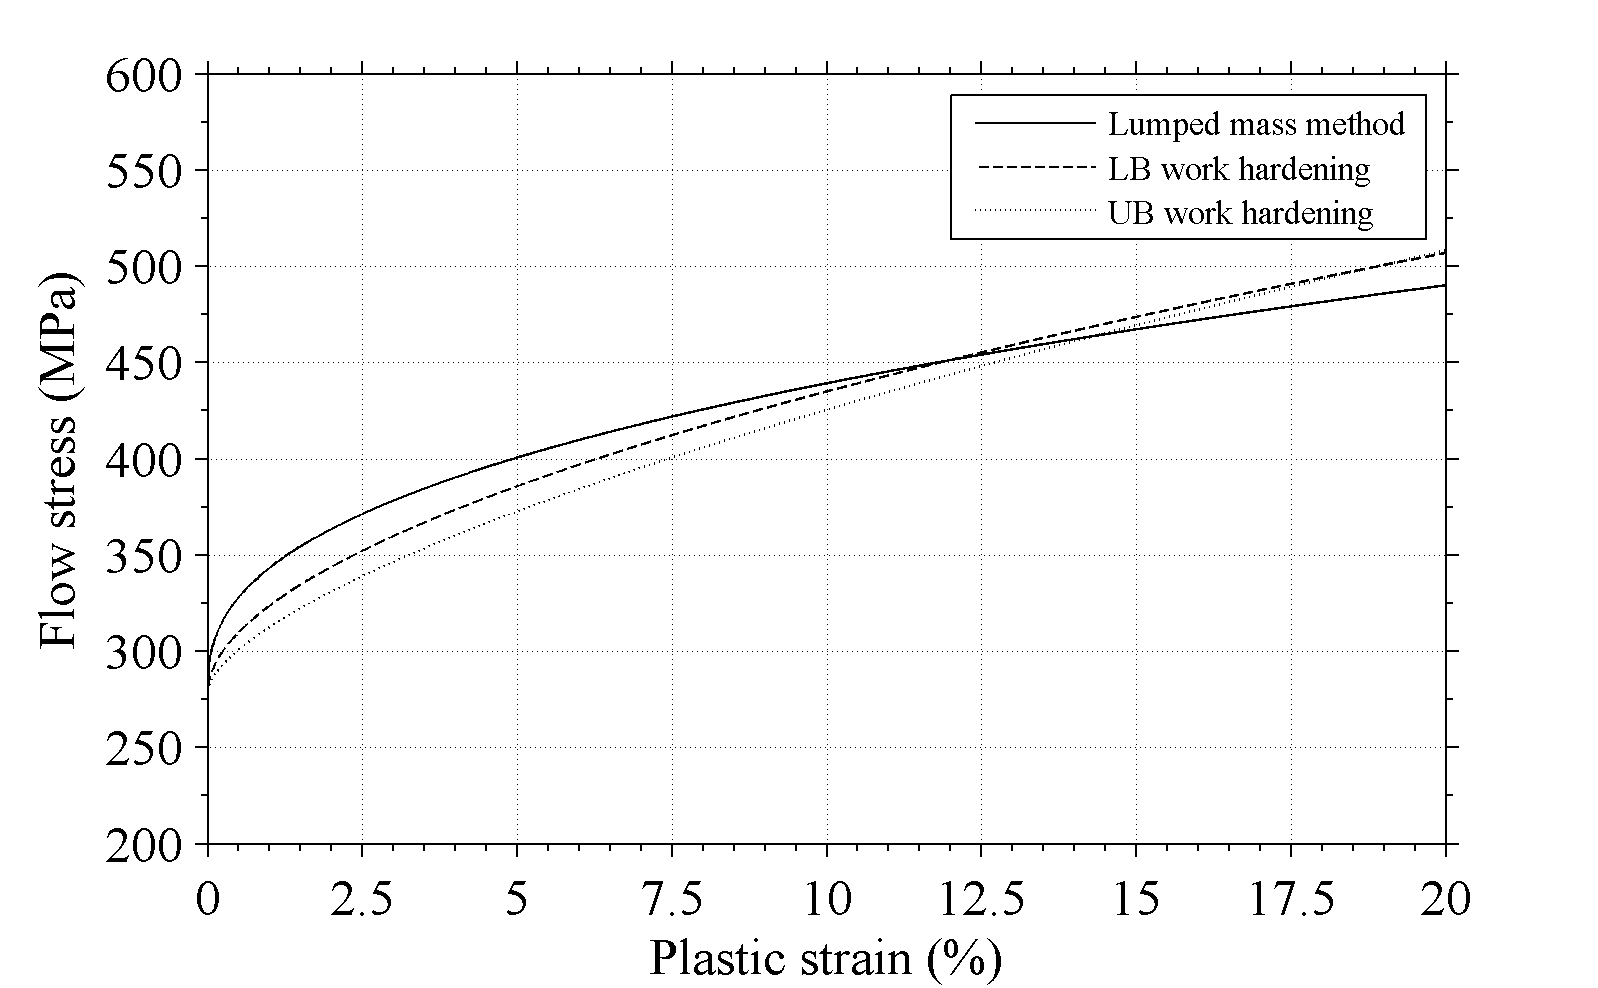
\includegraphics[width=.8\linewidth]{Figures/ModellingMethod/Workhardeningaltered}
	\caption[Work hardening response]{The plastic response of the nugget defined using the same initial yield stress (\textit{A}-parameter). However, the \textit{B} and \textit{n} parameters are based on the lumped mass method, the lower bound distributions, and the upper bound distributions.}
	\label{fig:Workhardeningeffect}
\end{figure}

In contrast, figure \ref{fig:Systematicmechs}e (simulation 9) shows that the predicted evolution of strain distribution correlates much more closely to the expected response. Indeed, it also correlates much more closely to the experimentally measured response (Figure \ref{fig:Systematicmechs}g). As mentioned earlier, the step change in the upper bond distribution of \textit{B} and \textit{n} parameters associated with the initial post-yield plastic response, induces a meso-scale stress concentration that is more diffuse than the lower bound distribution. This enables more elements associated with the nugget, TMAZ, and inner HAZ to accommodate the initial post-yield deformation strain. As a result, these inner regions can work harden up to the critical point in global deformation. Beyond this critical point, the flow stress of the inner regions of the HAZ, TMAZ, and nugget exceeds the flow stress in the outer HAZ, as illustrated in figure \ref{fig:ConstitutiveModels}. Hence, the overall distribution in flow stress in the outer HAZ, which is linked to the volume fraction of $\Omega$ phase, promotes the distribution of strain towards the centre of the weld. However, the mismatch in flow stress at the interface between the inner and outer HAZ, which is linked to the local capacity for work hardening, prevents strain localisation in the centre of the weld. Deformation strain is constrained to localise at the the interface of the inner and outer HAZ, which in 2139-T8 subject to FSW, is coincident with the geometric position of the hardness minima. 

It must be noted that the result of simulation 9, by definition, represents an overestimation of the evolution of strain distribution, owing to the user input work hardening response. Thus, there must exist some quantity of error in the prediction, which is evident by direct comparison with the experimentally measured response. However, the predicted results can be considered reliable as they do correlate reasonably well with the experimentally expected results. This result also indicates that the true distribution of work hardening properties in the weld is likely to be closer to the upper bound distribution of work hardening properties. This is a reasonable suggestion because the distribution of mechanical properties lies within the upper and lower bound property distributions, which are based on microstructural and mechanical property based observations of representative weld material. In addition, the result suggests that accurate and reliable estimation of the evolution of strain distribution necessarily requires an accurate description of both the initial yield response, and the work hardening response of the weld. Given that there is correlation between the prediction and experimental measurements, on both a macro and a local scale, the method used to define the local constitutive behaviour can be assumed to be reasonably effective. 

\subsubsection{Implications for failure prediction}
\label{SMDModellingstudyDiscussionPropertydistributionsImplications}
Assuming that the user input property distributions in simulation are both accurate and physically reasonable, the overall methodology must be numerically robust in order to assess the wider implications of its results. Figure \ref{fig:Systematicmechs}f shows that the numerical prediction from the mesh resolution study (simulation 10) is both qualitatively and quantitatively similar to figure \ref{fig:Systematicmechs}e (simulation 9). Initial yielding occurs within the elements associated with the nugget, TMAZ, and inner HAZ; as the local flow stress increases in these elements via work hardening, progressive yielding occurs in the immediately surrounding elements of the outer HAZ. The characteristic distribution of strain is increasing towards the centre of the weld. The characteristic distribution of strain increases up to a critical point, beyond which, strain begins to localise at the interface between the inner and outer HAZ. In addition, the overall distribution of absolute strain across the weld, and the peak values of strain, are comparable in figure \ref{fig:Systematicmechs}e-f. Hence, it can be assumed that sufficient mesh convergence has been achieved, and the prediction is relatively insensitive to mesh size. This indicates that the predictions using the method in simulation 9 are reliable from a numerical perspective.

In light of the numerical stability of the modelling method, it is likely that the mechanical property distributions across the weld are optimally represented by those used in simulation 9: a smooth distribution of hardness, and a stepped distribution in $k$, $B$, and $n$-parameters. As described previously, the property distributions correlate with the observed microstructural variation across the weld and are justified. The predicted values of directional plastic strain under these optimal user inputs (figure \ref{fig:Systematicmechs}e) have reasonable correlation with experiment (figure \ref{fig:Systematicmechs}g). As mentioned previously, failure in ductile materials is linked to plastic strain, hence, the optimal model provides a reasonable method for predicting the location of final failure. Indeed, the methodology developed in this chapter has been shown to produce improved prediction of the evolution of geometric strain distribution under uniaxial loading conditions compared to the lumped mass approach.

Whilst a particular failure criterion was not considered in this case, it is likely that the method developed here would provide a more accurate estimate of failure under loading compared to predictions using the lumped mass method, for a given failure criterion. This is because the lumped mass method leads causes numerical perturbations and instabilities when used to model welds with complex mechanical property distributions. In addition, there are numerous examples, in the public domain, of the use of detailed constitutive models in the lumped mass method to improve the reliability of numerical predictions of strain \cite{Kim2010,Kim2010a,Reis2004}. These models were used to assess the failure performance of welded structures, which is directly linked to the predicted quantity of local plastic strain. Given that the numerical prediction of local strain using the lumped mass approach is dominated by erroneous over-prediction of local strains, the efficacy of improving failure assessments through implementing detailed constitutive models is questionable. The studies in this chapter have shown that a relatively simple Johnson-Cook constitutive model can be used to produce accurate predictions of strain distribution if details of the material microstructure are accounted for. Indeed, the methodology developed here has been shown to produce more reliable predictions of local strain distribution compared to the lumped mass method, and represents an improved approach to assessing structural failure of welds.

\subsection{Chapter Summary}
\label{SMDSummary}
In this chapter, the results of a range of numerical studies based on the FEM, which aimed to predict the evolution of local strain distribution in friction stir welded 2139-T8 when loaded in simple uniaxial tension, were presented. The studies utilised a range of methods based on the lumped mass approach, whose application in the public domain is relatively common. In addition, an automated method for implementing complex mechanical property distributions, which are related to characteristic metallurgical properties, into FE based models of welds was described. This method was utilised to systematically study the effects of including details of local initial yield stress and work hardening response. Collectively, the studies indicated that simulations based on the lumped mass method enhanced intrinsic errors in the FEM, and that it could not be used to provide good quantitative correlation, on a local scale, with the experimentally measured strain response. Moreover, the numerical studies using the approach presented here indicate that successful FE based modelling of welds necessarily requires accurate definition of the local distribution of initial local yield stress and work hardening response. In addition, the studies provided an insight into the true nature of the distribution of mechanical properties, which tend to be diffuse in the outer regions of the HAZ, and more discrete in the inner regions of the inner HAZ, TMAZ, and nugget; this observation correlates with microstructural characterisation of the welded described in chapter \ref{ResultsMicrostructure} and the known link between microstructure and mechanical properties. The method presented here represents an improvement in numerical modelling approach, and has the theoretical property of being insensitive to either the loading configuration or geometric scaling. This also represents an improvement over existing lumped mass techniques, however, this property is tested in chapter \ref{ResultsApplications}.
% % % % % % % % % % % % % % % % % % % % % % % % % % % % % % % % % % % % % % % % % % % % % % % % % %
% % % % Conclusions
% % % % % % % % % % % % % % % % % % % % % % % % % % % % % % % % % % % % % % % % % % % % % % % % % %
\section{Conclusions}
\label{Conclusion}
In this study, an FE based modelling method, which incorporates element-wise material property variation to detail the strong material property gradients arising from the welding process, was utilised to predict the structural response of FSW 2139-T8 under complex loading configurations, including blast loading. The method requires an understanding of the strengthening mechanism variation in FSW 2139-T8 and is only feasible through automation of the mesh building process. The method utilised removes the need to calibrate models geometry to a particular loading configuration, rather it is calibrated to a normalised weld condition; this removes modelling errors which may arise when extending models to study structural performance under different loading configurations. Moreover, this allows the method to be used to study the effect of welding parameters on structural performance, potentially enabling numerical weld optimisation, which is theoretically applicable to any heat treatable aluminium alloy. The method has been verified experimentally using DIC for FSW 2139-T8 in under uniaxial tension. The method provides good correlation for strain evolution both globally and locally across the weld zone; this represents an improvement over existing techniques reported in the public domain. Furthermore, strong supporting experimental evidence has been generated which indicates that the method provides good qualitative and quantitative correlation with experimental evidence when extended to more complex loading configurations; this represents an improvement on modelling techniques available in the public domain.
%
%\begin{itemize}
%	\item Used FE to predict structural response with variable mat property gradients
%	\item variation in properties linked to strengthening mechanism variation
%	\item understanding mechanism variation has allowed detailed property gradients to be implemented using an automated mesh building process
%	\item We utilise a method whereby you remove calibration wrt loading configuration, rather to a normalised weld condition using Johnson Cook material models. Theoretically you can apply this to any weld.
%	\item the method accurately predicts behaviour in simple loading configurations and has been verified using DIC. In comparision to literature, there is both global and local quantitative correlation of strain evolution (geometrically and spatially)
%	\item method can be extended to complex structures and loading and provides good quantitative correlation with experimental evidence though a more detailed analysis using DIC may provide better data. Improvement from published literature
%	\item method can potentially provide better assessment of failure criterion as removes errors due to modelling itself
%\end{itemize}
%Basically the methodology is sound. Gives good results. Some issues are specifically addressed in Part II and will assumed to be linked to microstructure.

% % % % % % % % % % % % % % % % % % % % % % % % % % % % % % % % % % % % % % % % % % % % % % % % % %
% % % % Acknowledgements
% % % % % % % % % % % % % % % % % % % % % % % % % % % % % % % % % % % % % % % % % % % % % % % % % %
\section*{Acknowledgements}
\label{Acknowledgements}
The authors acknowledge the funding granted from EPSRC via the Advanced Metallic Systems CDT (EP/L016273/1) at the Universities of Manchester and Sheffield and LATEST2 program (EP/G022402/1). Further, the authors acknowledge DSTL for their contribution towards development of the FE method; Constellium for the provision and manufacture of materials; and Blastech for technical support during blast testing. Thanks also to David Strong and Bill Storrey for their contribution towards experimental testing; and Samuel Tammas-Williams, Tomas Brownsmith, and Richard Watson for their assistance in producing this paper. Please contact the corresponding author for access to the original data used in this article.

%% The Appendices part is started with the command \appendix;
%% appendix sections are then done as normal sections
%% \appendix

%% \section{}
%% \label{}

%% If you have bibdatabase file and want bibtex to generate the
%% bibitems, please use
%%

% % % % % % % % % % % % % % % % % % % % % % % % % % % % % % % % % % % % % % % % % % % % % % % % % %
% % % % References
% % % % % % % % % % % % % % % % % % % % % % % % % % % % % % % % % % % % % % % % % % % % % % % % % %
\section*{References}
  \bibliographystyle{elsarticle-num} 
  %Referencing system for in the office....
%  \bibliography{C:/Users/mbgm6aab/Documents/AdvancedMetallicSystemsCDT/PhD/Papers/library}
  	\bibliography{Bibliography/libraryFINALEDITHUGHSHERCLIFFCORRECTIONS}
 %Referencing system for home....
  %\bibliography{C:/Users/Public/Documents/AdvancedMetallicSystemsCDT/PhD/Papers/library}

%TODO Addressing Phil and Joe comments see below:
%The potential errors induced by the lumped mass approach are due to:
%* Yield stress step functions introduce a significant artifical strain localisation effect. This affects spatial strain response.
%* The lack of work hardening rate variation inhibits plastic response in the inner regions of the weld. Theoretically the stress strain curves can never cross over based on this assumption. Hence, this affects the temporal strain response. (Cross over of stress-strain curves)
%* Calibrating the meso-scale weld geometry to a particulaar loading configuration affects the geometric strain distribution and therfore affects the spatial strain response.
%
%
%The use of step functions in modelling can only be appropriate where physical variables are adequately represented using step functions. For properties such as yield stress variation, this is clearly inadequate as yield stress is known to demonstrate linear relationship with hardness. For parameters such as the work hardening rate, where there is no clear relationship with any other measureable parameters in the literature, a suitable modelling function must be defined based on logic and scientific understanding. 
%
%From examining property variation obtained by curve fitting to measured mech props of the outer HAZ, there appears to be little discernible variation in work hardening rate. However, in the inner region of the HAZ there does appear to be a relatively big step change in work hardening rate. From TEM observation, it appears that this step change coincides with the dissolution of precipitates and annihilation of  dislocation structures on a local scale within the inner HAZ. In the nugget region, there also appears to be another relatively big jump in the work hardening rate fitted to measured mech props. Further, TEM observation indicates that precipitates have dissolved, dislocation structures are annihilated and there is additional grain refinement; this is another distinct change in microstructure. 
%
%Experimental observations appear to indicate that there is little variation in work hardening rate across the weld except where there are distinct changes to the microstructure. If there are distinct changes in observed microstructure and measured properties, it would be reasonably appropriate to assume that a step function would adequately describe those specific properties (i.e the work hardening rate). Assuming any other relationship, such as a linear relationship with hardness, would be inappropriate from the limited number of data points generated and lack of evidence within the literature. Whilst this modelling assumption may potentially induce erroneous work hardening behaviour in the model, the method does incorporate some degree of property variation that is linked to physical observations by TEM. This may be a more physically reasonable modelling assumption in comparison to the lumped mass method where work hardening is assumed not to vary across the weld. Additionally, there is wide evidence in the literature for variation in the work hardening rate across a weld which is ignored in the lumped mass method.
%
%In modelling, a representative solution can be found if the parameters of a model are varied in such a way that the output response matched experimental evidence. Theoretically, there will exist a wide set of parameter combinations that give similar outputs. For example consider the model A+Bep^n=Ys  However, they do not accurately represent reality and hence when models are extended to more complex configurations it is unlikely that good correlation can be found with experimental evidence. The modelling simplifications made in this study are based on experimental evidence and are physically justifiable. Hence, it is unsurprising that a relatively accurate description of weld properties and geometry that is not calibrated to any particular loading condition would lead to a relatively accurate description of structural response under generic loading configurations.
%
%
%Why do I use some smooth and some step functions. Need to add in my criticism of lumped mass method that there is no supporting evidence for particular parameters to demonstrate smooth or step functions. For yield stress there is evidence for smooth functions (liunear relationship with Hv). For work hardening rate, the variation in HAZ is gradual, but where distinct changes occur there is a relatively large change in property. The erroneous predictions using lumped mass method are likely due to a combination of step function of yield stess, zero variation in work hardening rate, and calibration of meso-scale weld geometry to a particular loading condition. A combination of all three assumptions rather than any particular one.
%
%In my work I have introduced smoother gradients in yield stress, removed calibration of weld geometry to a particular loading condition and introduced variation to work hardening rate and other parameters based on TEM observations and measured mechanical properties.


%% else use the following coding to input the bibitems directly in the
%% TeX file.

%\begin{thebibliography}{00}

%% \bibitem{label}
%% Text of bibliographic item

%\bibitem{}

%\end{thebibliography}
\end{document}
\endinput
%%
%% End of file `elsarticle-template-num.tex'.
